\documentclass[10pt]{article}

%%%%%%%%%%%%%%%%%%%%%%%%%%%%%%%%%%%%%%%%%%%%%%%%%%%%%%%%%%%%%%%%%

\usepackage[utf8]{inputenc}
\usepackage[T1]{fontenc}
\usepackage[paper=a4paper,left=0.5in, right=0.5in]{geometry} % http://ctan.org/pkg/geometry
\usepackage{graphicx} % add images
\usepackage{subfig} % to put images side by side
\usepackage[french]{babel} % langue francaise et symboles
\usepackage{hyperref} % pour les hyper-liens
\usepackage[acronym, toc, nogroupskip]{glossaries} % permet de construire un glossaire pour les abréviations utilisés
\usepackage[style=nature]{biblatex} % Imports biblatex package
\usepackage{listings} % pour écrire des chuncks de code
\usepackage[table]{xcolor}
\usepackage{titlesec} % to customize chapters, sections and subsections style in an easy way
\usepackage{rotating} % landscape orientation for pages
\usepackage{float} % for floating elements
\usepackage{makecell} % break line in tabular cell
\usepackage{pifont} % pour les listes
\usepackage{booktabs} % pour les tableaux
\usepackage{lipsum} % pour tester la mise en page
\usepackage{xurl} % for external links

%%%%%%%%%%%%%%%%%%%%%%%%%%%%%%%%%%%%%%%%%%%%%%%%%%%%%%%%%%%%%%%%%

\title{\huge{\textbf{Annotation des éléments transposables du moustique tigre \textit{Aedes albopictus}}}}

\author{\makebox[.9\textwidth]{\textbf{Auteur:}}\\Tommaso\\ BARBERIS \\ \texttt{tommaso.barberis@etu.univ-lyon1.fr} \and \textbf{Encadrant:}\\Matthieu\\ BOULESTEIX \\ \texttt{matthieu.boulesteix@univ-lyon1.fr}}

\date{Janvier - Juillet 2022}

%%%%%%%%%%%%%%%%%%%%%%%%%%%%%%%%%%%%%%%%%%%%%%%%%%%%%%%%%%%%%%%%

% hypperef setup
\hypersetup{
    colorlinks=true,
    linkcolor=black,
    urlcolor=blue,
    citecolor=blue,
    linktoc=all,
}

% glossaries setup
\makeglossaries
\newacronym{et}{ET}{éléments transposables}
\newacronym{ltr}{LTR}{Long Terminal Repeats}
\newacronym{tir}{TIR}{Terminal Inverted Repeats}
\newacronym{tsd}{TSD}{Target Site Duplication}
\newacronym{tip}{TIPs}{Transposon Insertion Polymorphisms}
\newacronym{th}{TH}{transferts horizontaux}
\newacronym{shr}{ShR}{short reads}
\newacronym{lr}{LR}{long reads}
\newacronym{sr}{SR}{Split-Read}
\newacronym{drp}{DRP}{Discordant Read Pair}
\newacronym{octfta}{OCTFTA}{OneCodeToFindThemAll}
\newacronym{line}{LINE}{Long Interspersed Nuclear Elements}
\newacronym{sine}{SINE}{Short Interspersed Nuclear Elements}
\newacronym{mite}{MITE}{Miniature Inverted-repeat Transposable Elements}
\newacronym{ssr}{SSR}{Simple Sequence Repeats}
\newacronym{orf}{ORF}{Open Reading Frame}
\newacronym{pbs}{PBS}{Primer Binding Site}
\newacronym{rc}{RC}{Rolling-circle (Helitron)}
\newacronym{rt}{RT}{Retrotranscriptase}
\newacronym{ple}{PLE}{Penelope-Like Element}

% biblatex setup
\addbibresource{ref.bib} % Import the bibliography file
\appto{\bibsetup}{\raggedright}

% xcolor setup
\definecolor{codegreen}{rgb}{0,0.6,0}
\definecolor{codegray}{rgb}{0.5,0.5,0.5}
\definecolor{codepurple}{rgb}{0.58,0,0.82}
\definecolor{backcolour}{rgb}{0.95,0.95,0.92}

% listing setup
\lstdefinestyle{mystyle}{
    backgroundcolor=\color{white},   
    commentstyle=\color{codegreen},
    keywordstyle=\color{magenta},
    numberstyle=\tiny\color{codegray},
    stringstyle=\color{codepurple},
    basicstyle=\ttfamily\footnotesize,
    breakatwhitespace=false,         
    breaklines=true,                 
    captionpos=b,                    
    keepspaces=true,                 
    numbers=left,                    
    numbersep=5pt,                  
    showspaces=false,                
    showstringspaces=false,
    showtabs=false,                  
    tabsize=2
}

\lstset{style=mystyle}

% titlesec setup
\titlespacing\section{0pt}{50pt}{25pt}
\titlespacing\subsection{0pt}{30pt}{20pt}

%%%%%%%%%%%%%%%%%%%%%%%%%%%%%%%%%%%%%%%%%%%%%%%%%%%%%%%%%%%%%%%%

\begin{document}

%%%%%%%%%%%%%%%%%%%%%%%%%%%%%%%%%%%%%%%%%%%%%%%%%%%%%%%%%%%%%%%%
%% Commandes qui nécessitent d'être appelé après le début du document

% ref setup
\renewcommand{\tableautorefname}{\textsc{Tableau}} 
\renewcommand{\figureautorefname}{\textsc{Figure}} 
\renewcommand{\sectionautorefname}{\textsc{Section}} 
\renewcommand{\paragraphautorefname}{\textsc{Paragraphe}} 
\renewcommand{\subsectionautorefname}{\textsc{Sous-section}}
\renewcommand{\subparagraphautorefname}{\textsc{Sous-paragraphe}}


\newcommand{\beginglossary}{%
        \setcounter{table}{0}
        \renewcommand{\thetable}{G\arabic{table}}%
        \setcounter{figure}{0}
        \renewcommand{\thefigure}{G\arabic{figure}}%
        \setcounter{lstlisting}{0}
        \renewcommand{\thelstlisting}{G\arabic{lstlisting}}%
     }
 
 \newcommand{\begincentralsection}{%
    \setcounter{table}{0}
    \renewcommand{\thetable}{\arabic{table}}%
    \setcounter{figure}{0}
    \renewcommand{\thefigure}{\arabic{figure}}%
    \setcounter{lstlisting}{0}
    \renewcommand{\thelstlisting}{\arabic{lstlisting}}%
 }
 
\newcommand{\beginsupplement}{%
        \setcounter{table}{0}
        \renewcommand{\thetable}{S\arabic{table}}%
        \setcounter{figure}{0}
        \renewcommand{\thefigure}{S\arabic{figure}}%
        \setcounter{lstlisting}{0}
        \renewcommand{\thelstlisting}{S\arabic{lstlisting}}%
     }
     
\renewcommand{\lstlistingname}{\textsc{Code}}

% for external link section
\newcounter{link}
\setcounter{link}{0}
\newcommand*{\linkautorefname}{\textsc{Lien~}}
\newcommand*{\extlink}{\textsc{\linkautorefname\arabic{link}}}
\newenvironment{link}[1][]{
\refstepcounter{link}%
\noindent\textsc{\linkautorefname\thelink}
}
%%%%%%%%%%%%%%%%%%%%%%%%%%%%%%%%%%%%%%%%%%%%%%%%%%%%%%%%%%%%%%%%

\begin{titlepage}
    
    % 
\includegraphics[width=0.55\textwidth]{img/logo/bioinfo@lyon_logo.png}
    % 
\includegraphics[width=0.2\textwidth]{img/logo/cnrs_logo.png}
    % 
\includegraphics[width=0.2\textwidth]{img/logo/lbbe_logo.png}
    
    \begin{figure}
        \centering
        \subfloat{{
\includegraphics[width=0.2\textwidth]{img/logo/lbbe_logo.png}}}
        \hspace{0.5cm}
        \subfloat{{
\includegraphics[width=0.15\textwidth]{img/logo/cnrs_logo.png}}}
        \hspace{0.5cm}
        \subfloat{{
\includegraphics[width=0.4\textwidth]{img/logo/bioinfo@lyon_logo.png} }}
    \end{figure}
    
    \vspace{2cm}
    
    \maketitle
    \thispagestyle{empty} % no page number on this page
\end{titlepage}

\newgeometry{top=1in,bottom=1in,right=1in,left=1in}

\begin{abstract}
\phantomsection
\addcontentsline{toc}{section}{Résumé} % add the abstract to the content table

\textit{Aedes albopictus}, mieux sous le nom de moustique tigre, est un des vecteurs de certaines maladies virales, comme la dengue et le chikungunya. Des études récentes on montré que son génome est peuplé de nombreux \acrfull{et}. \\
Dans ce stage, nous nous sommes ainsi consacré à leur annotation, à l'aide d'une double approche homologie - \textit{de novo} et, à la construction de la librairie d'\acrshort{et} conséquente. Les séquences contenues dans la librairie ont été polies à l'aide d'un pipeline conçu pour l'occasion et, classifiées pour connaître le paysage d'\acrshort{et} du génome de cette espèce.
\end{abstract}

\pagenumbering{roman}
\vfill
\begin{center}
    \footnotesize{This work was performed using the computing facilities of the CC LBBE/PRABI.}
\end{center}
\newpage

\renewcommand*\contentsname{Table des matières}
\phantomsection
\tableofcontents
\addcontentsline{toc}{section}{Table des matières} 

\newpage

\renewcommand{\listfigurename}{Table des figures} % rename list of figures
\phantomsection
\listoffigures
\addcontentsline{toc}{section}{\listfigurename} % add the list to the content table

\newpage

\renewcommand{\listtablename}{Table des tableaux} % rename list of tables
\phantomsection
\listoftables
\addcontentsline{toc}{section}{\listtablename} % add the list to the content table

\newpage

\printglossary[type=\acronymtype, title=Abréviations]

\newpage

\phantomsection
\newcounter{glossarysection}
\renewcommand{\theglossarysection}{Glossaire}
\refstepcounter{glossarysection}
\label{sec:gloss}
\section*{Glossaire}
\addcontentsline{toc}{section}{Glossaire}
\beginglossary

\textbf{\acrfull{tir}}: il s'agit d'une répétition sur les extrémités d'une séquence, où une extrémité est le complémentaire inverse de l'autre. \\
    
    \bigskip
    
    \begin{figure}[H]
        \centering
        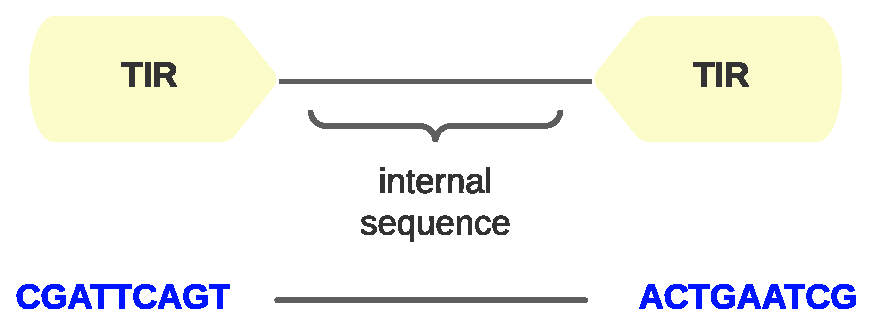
\includegraphics[width=0.5\textwidth]{img/misc/TIR.eps}
        \caption{Exemple de \acrshort{tir}.}
        \label{fig:TIR_exemple}
    \end{figure}
    
    \bigskip
    
\textbf{\acrfull{ltr}}: c'est une paire de séquences d'ADN identiques, qui peuvent avoir une longueur jusqu'à quelques centaines de nucléotides. Dans les rétrotransposons (Classe I) à \acrshort{ltr}, ces deux séquences se trouvent aux extrémités 5' et 3' de la séquence. \\

\bigskip

\begin{figure}[H]
    \centering
    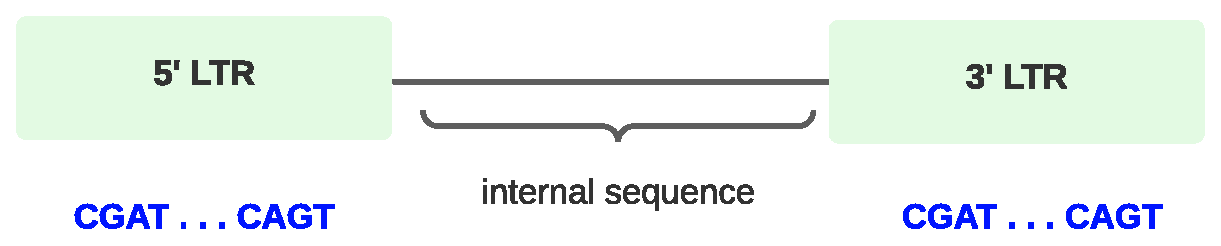
\includegraphics[width=0.5\textwidth]{img/misc/LTR.eps}
    \caption{Exemple de \acrshort{ltr}.}
    \label{fig:LTR_example}
\end{figure}

\bigskip

\textbf{\acrfull{pbs}}: il s'agit de la région nucléotidique où des amorces d'ADN peuvent venir se hybrider pour permettre à la réplication d'avoir lieu. Dans les \acrshort{et} du type \acrshort{ltr}, le \acrshort{pbs} a une taille qui est comprise entre 20 et 25 nucléotides, il est le complémentaire d'un \textit{tARN} et se trouve en 3', à quelque nucléotide près, du \acrshort{ltr} en 5'. Il est donc utilisé comme amorce pour la \acrfull{rt} \cite{wicker}. \\
    
\bigskip

\begin{figure}[H]
    \centering
    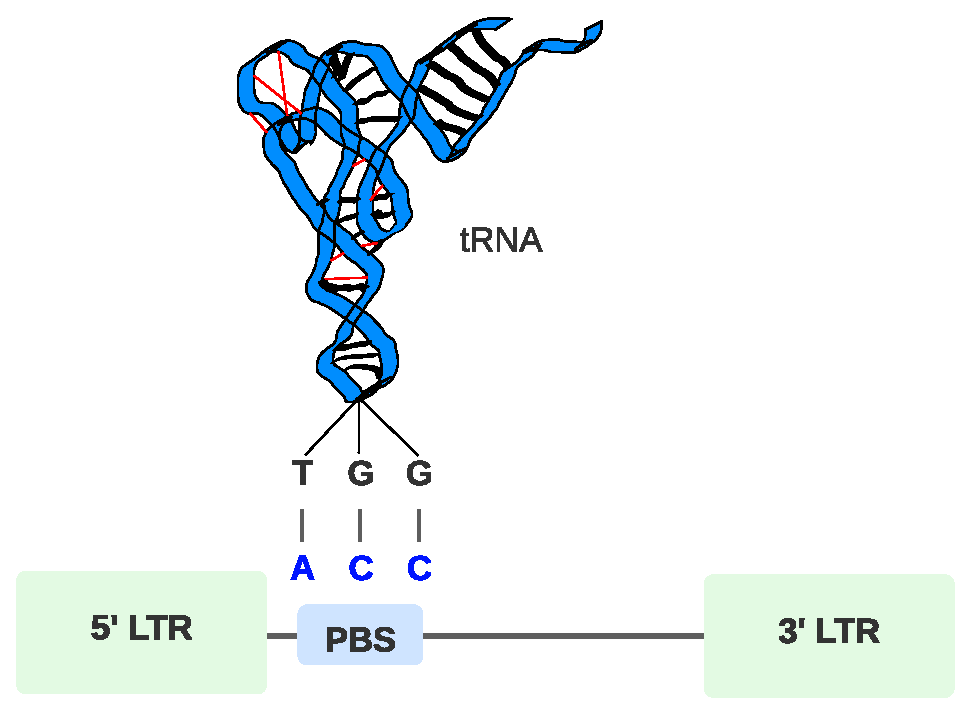
\includegraphics[width=0.5\textwidth]{img/misc/PBS.eps}
    \caption{Exemple de \acrshort{pbs}.}
    \label{fig:pbs_exemple}
\end{figure}

\bigskip

\textbf{\acrfull{tsd}}: il s'agit généralement d'une courte répétition directe qui est obtenue sur les régions flanquantes d'\acrshort{et} après son insertion. \\

\bigskip

\begin{figure}[H]
    \centering
    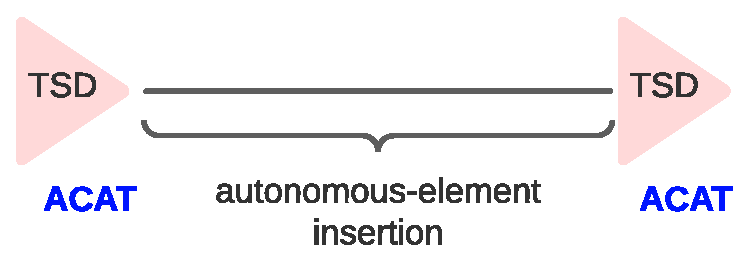
\includegraphics[width=0.5\textwidth]{img/misc/TSD.eps}
    \caption{Exemple de \acrshort{tsd}.}
    \label{fig:TSD_example}
\end{figure}


%TODO: rajouter glossaire pour les domaines protéiques

\newpage

\phantomsection
\section*{Logiciels et Bases de données}
\addcontentsline{toc}{section}{Logiciels et Bases de données}

\paragraph{Logiciels}
\begin{itemize}
    \item \texttt{RepeatModeler - 2.0.2} \\
    Commentaire de la ligne \texttt{140}:% Flynn et al.
\begin{lstlisting}[language=perl]
 # use Devel::Size qw(size total\_size);
\end{lstlisting}
    \begin{itemize}
        \item \texttt{RECON - 1.08} % Bao Z. and Eddy S.R. 2002
        \item \texttt{RepeatScout - 1.0.6} % Price A.L. et al 2005
        \item \texttt{Tandem Repeats Finder - 4.09} % G. Benson 1999
        \item \texttt{RMBlast - 2.11.0} % citer quoi? utilisé comme défaut par RepeatMasker
        \item \texttt{LtrHarvest (genometools) - 1.5.9} % David Ellinghaus 2008
        \begin{itemize}
            \item \url{https://github.com/genometools/genometools/pull/917/files}, changements sur les fichiers:
            \begin{itemize}
                \item \texttt{src/ltr/ltr\_cluster\_prepare\_seq\_visitor.c}
                \item \texttt{src/ltr/ltr\_cluster\_stream.c}
                \item \texttt{src/match/eis-bwtseq-context.c})
            \end{itemize} 
            \item \url{https://github.com/genometools/genometools/pull/857/files}, changements sur les fichiers:
            \begin{itemize}
                \item \texttt{src/extended/gff3\_escaping.c}
                \item \texttt{src/match/eis-bwtseq-context.c}
            \end{itemize}
            \item compilé avec la ligne de code suivante: 
\begin{lstlisting}[language=bash]
make threads=yes cairo=no
\end{lstlisting}
        \end{itemize}
        \item \texttt{LTR\_retriever - 2.6} % Ou S. and Jiang N. (2018)
        \begin{itemize}
            \item \texttt{BLAST+ package - 2.12.0}
            \item \texttt{cdhit - 4.8.1}
            \item \texttt{HMMER - 3.3.2}
            \item \texttt{RepeatMasker - 4.1.2 p1}
            \begin{itemize}
                \item Module \texttt{Python} installé via \texttt{pip}: \texttt{h5py - 3.6.0}
            \end{itemize}
        \end{itemize}
        \item \texttt{MAFFT - 7.490}
        \item \texttt{NINJA - 0.98-cluster\_only}
        \item \texttt{UCSC TwoBit Tools - 1.04.00}
        \item modules \texttt{Perl} (compilés à partir du code source):
        \begin{itemize}
            \item \texttt{JSON - 4.05}
        \end{itemize}
    \end{itemize}
    \item \texttt{MITE-Tracker - commit 23ee261} (avec \texttt{python3})
    \begin{itemize}
        \item \texttt{vsearch - 2.7.1}
        \item modules \texttt{Python} (installés via \texttt{conda}):
        \begin{itemize}
            \item \texttt{biopython - 1.79}
            \item \texttt{numpy - 1.22.1}
            \item \texttt{pandas - 1.4.0}
        \end{itemize}
    \end{itemize}
    \item \texttt{singularity - 3.7.2}
    \item \texttt{conda - 4.12.0}
    \item \texttt{EDTA - 2.0.0} (avec \textit{perl - 5.26.2})
    %\item \texttt{Earl Grey - 1.2} (Dépendances: \texttt{RepeatModeler} et \texttt{RepeatMasker})
    \item \texttt{One code to find them all - 1.0}
    %\item \texttt{So2 TE Bioinformatic ressources (Parisot et al. 2020) - commit ab60c10}
    %\begin{itemize}
    %    \item \texttt{GNU Parallel - 20220222}
    %    \item \texttt{Mothur - 1.45.2}
    %\end{itemize}
    \item \texttt{bedops - 2.4.40}
    \item \texttt{samtools - 1.15}
    \item \texttt{bedtools - 2.30.0}
    %\item \texttt{MeShClust - commit 3d2a699} (à partir du répertoire: \url{https://github.com/BioinformaticsToolsmith/Identity})
    \item \texttt{seqtk - 1.3}
    %\item \texttt{SRA toolkit - 3.0.0}
    %\item \texttt{FastQC - 0.11.9} \\
    %\url{https://www.bioinformatics.babraham.ac.uk/projects/fastqc/fastqc_v0.11.9.zip}
    \item \texttt{ART - 2.5.8}
    %\item \texttt{GATK - 4.2.5.0}
    %\item \texttt{gsutil - 375.0.0}
    %\begin{itemize}
    %    \item \texttt{crcmod - 1.7} (module \texttt{Python})
    %\end{itemize}
    \item \texttt{DeepTE - commit 69a7465}
    \item \texttt{dnaPipeTE - v.1.3.1\_07}
    \item \texttt{CIAlign - 1.0.15}
    \item \texttt{TE-Aid - v.0-dev}
\end{itemize}

\paragraph{Bases de données}
\begin{itemize}
    \item \texttt{RepBase - 25.08}
    \item \texttt{Dfam - 3.5}
\end{itemize}

%\vspace{0.5cm}


\newpage

\pagenumbering{arabic}
\begincentralsection

\section{Introduction}

S'intéresser aux mécanismes d'évolution et d'adaptation d'une espèce est le point clé de la biologie évolutive. Celle-ci permet d'étudier et comprendre en détail le comportement ainsi que les environnements où l'espèce habite. 
Par exemple, elle permet d'étudier les mécanismes évolutifs qui ont permis au moustique tigre \textit{Aedes albopictus}  de coloniser le monde entier dans les dernières décennies. \\ 

Le moustique tigre (\figureautorefname{ \ref{fig:aedes_photo}}), est un insecte diptère de la famille \textit{Culicidae} provenant de l'Asie du sud-est qui peut être reconnu facilement grâce à ses rayures blanches et noires qu'il porte sur les pattes. Il est de couleur noir et il porte sur le thorax une ligne blanche. Le genre \textit{Aedes} regroupe environ 263 espèces dont aussi \textit{Aedes aegypti}, lequel se distingue de l'espèce sœur par ses marque blanches en forme de lyre sur le thorax et sa couleur marron. \\

\bigskip

\begin{figure}[h]
    \centering
    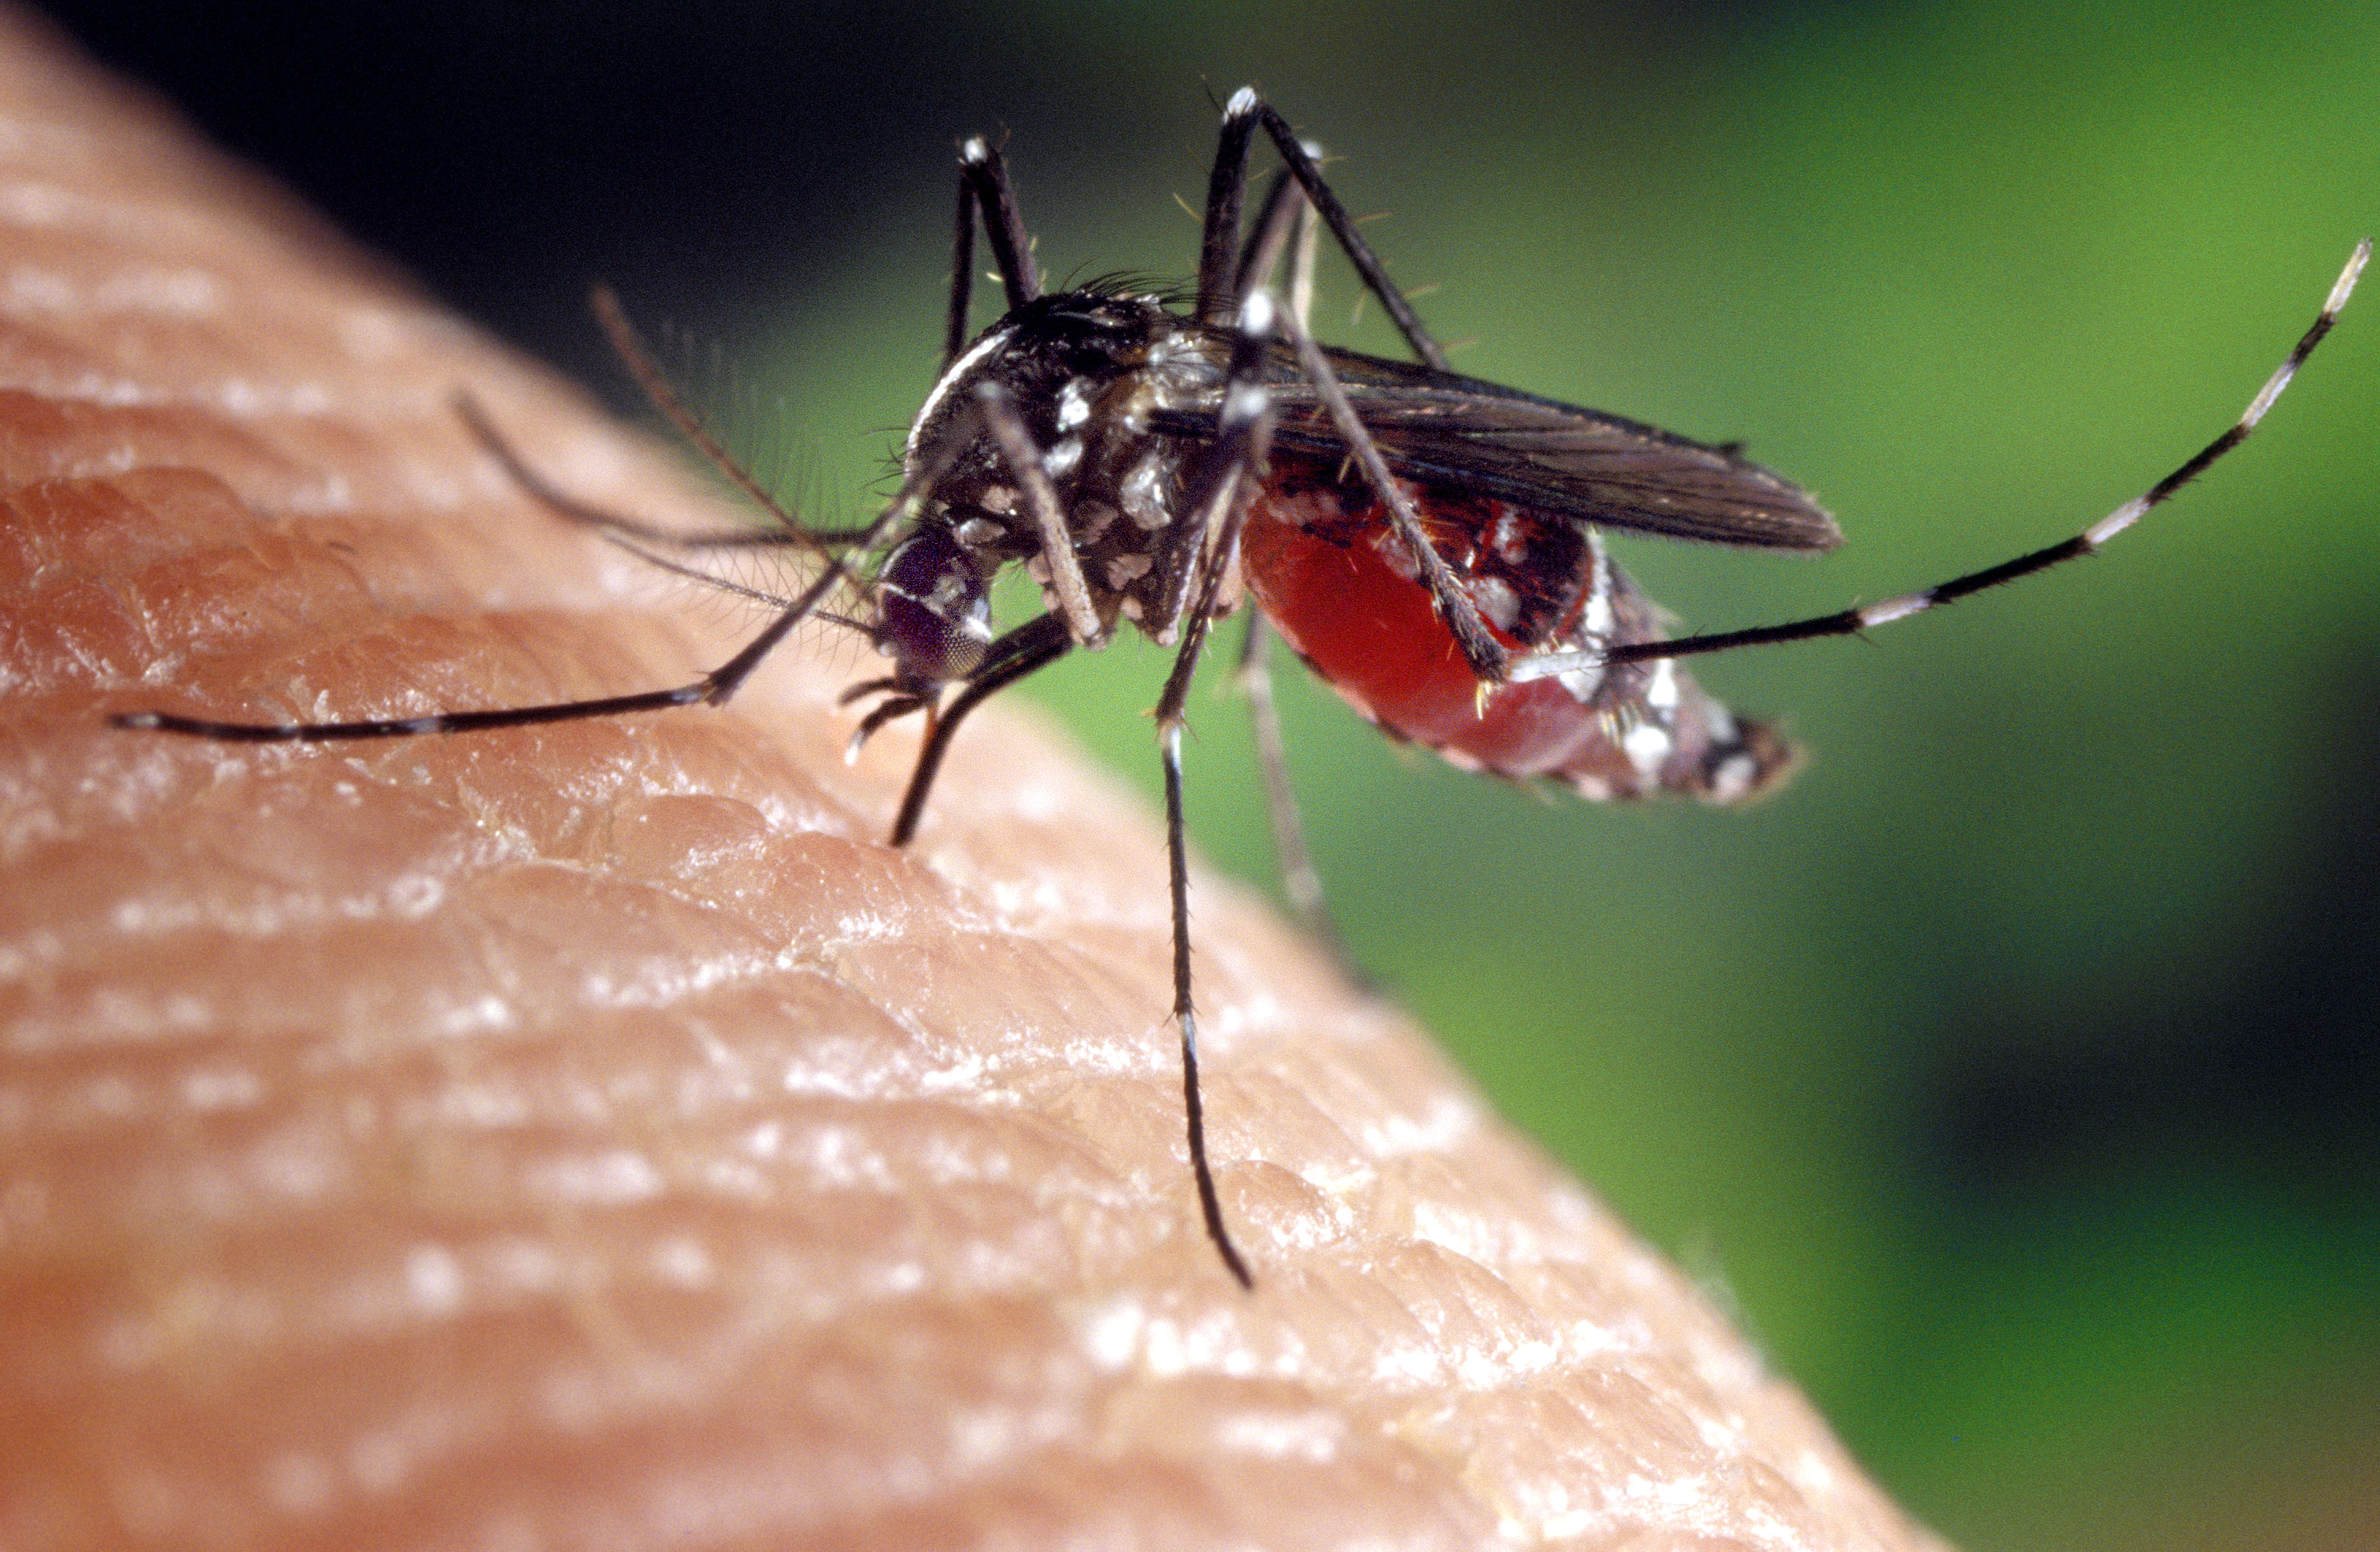
\includegraphics[width=0.5\textwidth]{img/misc/aedes_albopictus.jpg}
    \caption{Image représentative du moustique tigre.}
    \caption*{\scriptsize{Photo DR}}
    \label{fig:aedes_photo}
\end{figure}

\bigskip

\paragraph{Pourquoi étudier l'évolution de \textit{Ae. albopictus}?} L'étude d'\textit{Ae. albopictus} a pris une importance depuis sa propagation dans le monde entier, en devenant un sujet de recherche de plus en plus ciblé, mais également, du fait de son implication en tant que vecteur principal de certains arbovirus (virus de la dengue et du chikungunya) lors d'épidémies récentes \cite{paupy_aedes_2009}. \\
Dans les 30 dernières années, il a colonisé l'Afrique, l'Europe et l'Amérique à partir de l'Asie de l'Est, principalement grâce au commerce de pneus usagés, lesquels sembleraient être un endroit préférentiel pour la ponte des oeufs \cite{porretta_glacial_2012}\cite{Reiter1998AedesAA}.  \\

Le moustique tigre, comme plusieurs autres espèces du genre \textit{Aedes}, est vecteur de maladies infectieuses  d'origine virale, on a déjà cité la dengue et le chikungunya, mais on retrouve aussi beaucoup d'autres virus \cite{gratz_critical_2004}\cite{mckenzie_aedes_2019} (parmi eux, on suspecte aussi la transmission du virus zika). Aujourd'hui plusieurs de ces maladies n'ont pas un traitement spécifique disponible, pour cette raison, le contrôle des vecteurs reste la meilleure stratégie pour les contrer. \\
La biologie évolutive permet notamment d'étudier les caractéristiques d'\textit{Aedes albopictus} qui lui ont permis de survivre et de s'adapter à des environnements qui lui étaient défavorables dans le passé et, ainsi potentiellement d'imaginer des nouvelles méthodes de lutte. \\
Il a pu s'adapter rapidement en Occident malgré le climat tempéré, par opposition au climat tropical et humide de sa région d'origine. Plusieurs hypothèses sur l'acquisition de cette nouvelle capacité peuvent être faites, comme la symbiose avec un nouveau partenaire (viral ou bactérien) ou encore l'influence du changement climatique. \\
Cependant, ici on s'intéressera uniquement à l'adaptation de l'espèce via des événements évolutifs provoqués par des structures génomiques particulières, appelés \acrfull{et} lesquels seront décrits dans le paragraphe suivant. \\

\bigskip

\paragraph{Les \acrlong{et}}\label{par:explanation_te} Les \acrlong{et} sont des séquences d'ADN qui possèdent la capacité de se déplacer/répliquer au sein du génome sur lequel ils se trouvent, grâce à un mécanisme de duplication \og copy-and-paste \fg{} \cite{bourque_ten_2018} ou de déplacement \og cut-and-paste \fg{}. Cette propriété qui les rend mobiles, peut être à l'origine de modifications génomiques lesquelles peuvent avoir un impact sur  l'évolution de l'espèce. \\

\bigskip

\begin{figure}[h]
    \centering
    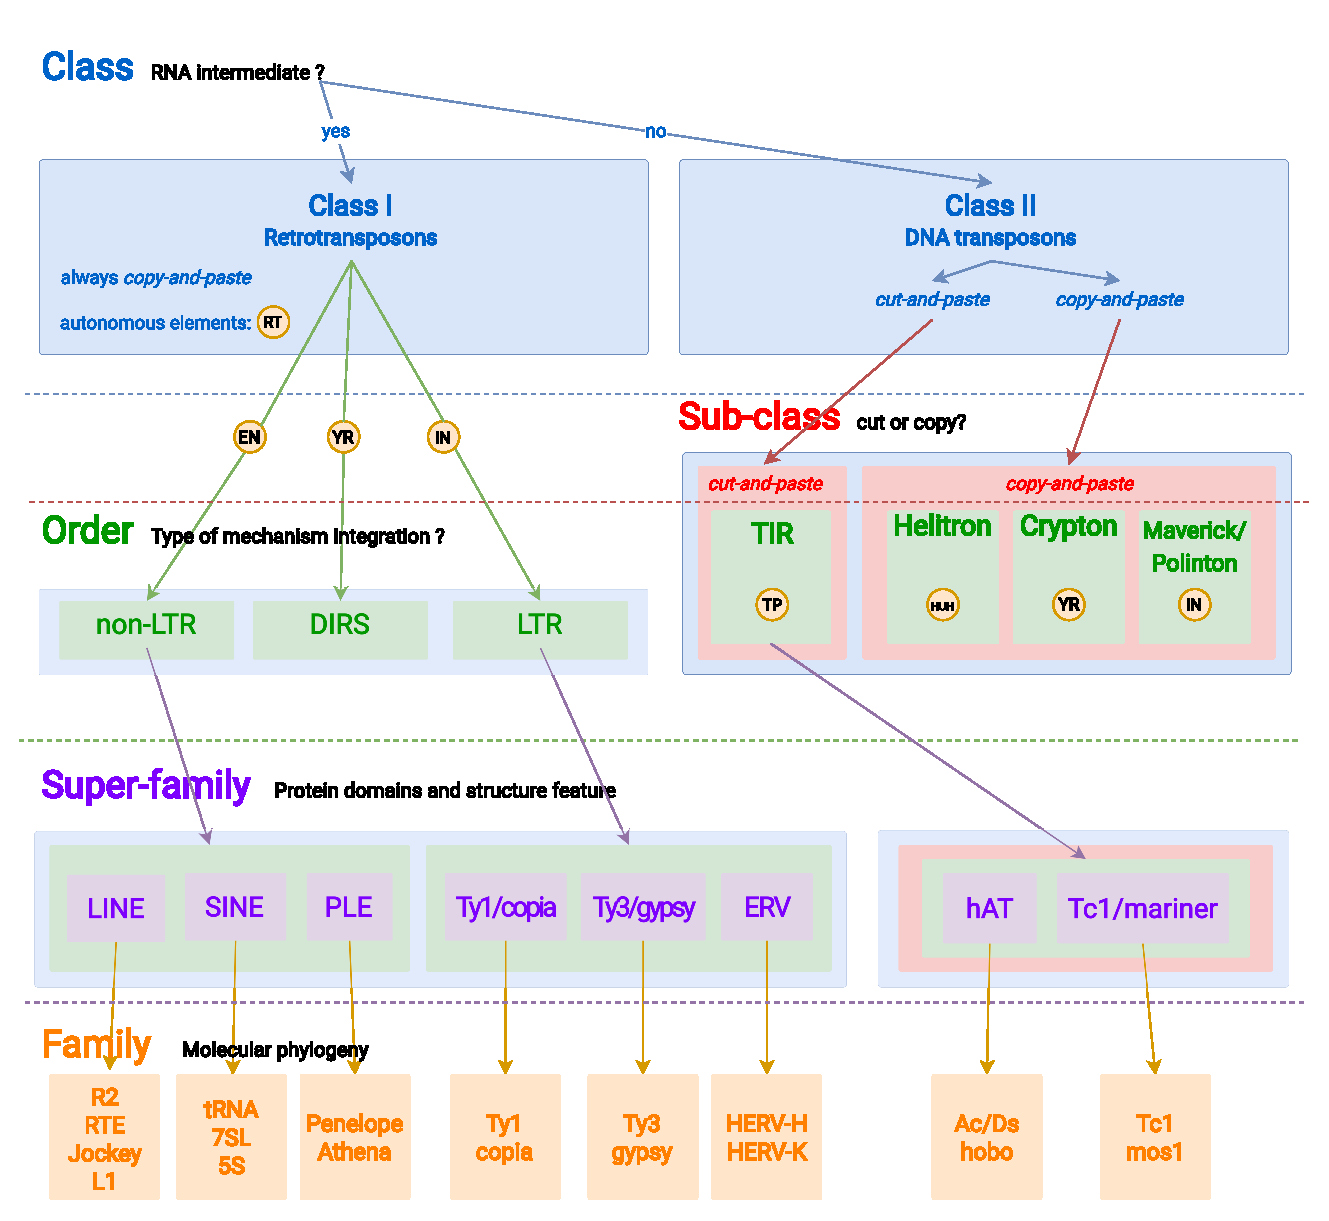
\includegraphics[width=0.9\textwidth]{img/misc/transposable_elements.eps}
    \caption{Classification des \acrfull{et}.}
    \caption*{\scriptsize
    Chaque couleur (bleu, rouge, vert, violet et orange) représente un niveau dans la hiérarchie. Les ronds orange représentent les domaines protéiques (pour les éléments autonomes) associés au niveau considéré. \\
    RT: retrotranscriptase, EN: endonuclease, YR: recombinase à tyrosine, IN: integrase, TP: transposase, HUH: hélicase. \\
    Sources: \textit{Wicker et al.} \cite{wicker}, \textit{Borque et al.} \cite{bourque_ten_2018}.
    }
    
    \label{fig:classif_et}
\end{figure}

\bigskip

Les \acrlong{et} ont été découverts par Barbara \textbf{McClintock} dans les années 1940. Dans ses travaux, elle a réussi, en particulier, à comprendre le rôle des \acrshort{et} dans la cassure chromosomique et ainsi dans le changement phénotypique (couleur de la graine) chez le maïs \cite{mcclintock_origin_1950}. Depuis, ce qui été considéré avant comme de l'ADN \og poubelle \fg{}, en raison de sa nature hautement répétée  et de l'absence de fonctions biologiques évidentes pour l'organisme, est aujourd'hui de plus en plus étudié. \\
La plupart des eucaryotes possèdent des \acrlong{et} et, leur proportion au sein du génome peut varier d'une espèce à l'autre \cite{wells_field_2020}. Par exemple, le génome du maïs a un contenu en \acrshort{et} très élévé (85\% du génome) \cite{schnable_b73_2009} alors que le génome humain possède 45\% d'\acrshort{et} \cite{lander_initial_2001}  et le génome de \textit{Drosophila melanogaster} n'en possède "que" 20\% \cite{mccullers_transposable_2017}. \\
Les \acrshort{et} peuvent être organisés selon une vraie hiérarchie \cite{wicker} (\figureautorefname{ \ref{fig:classif_et}}). Ils se divisent en deux classes principales, les éléments de classe I, ou rétrotransposons, qui utilisent un intermédiaire à ARN pour se déplacer et, les éléments de classe II, ou transposons à ADN. Tous les éléments de classe I utilisent un mécanisme de réplication \textit{ \og copy-and-paste \fg{}}, alors que dans les classe II on retrouve aussi des \acrshort{et} utilisant un mécanisme de \textit{\og cut-and-paste \fg{}}. Cette discrimination est souvent utilisée pour séparer les transposons à ADN en deux sub-classes. \\
Chaque classe (ou sub-classe) se divise ensuite en plusieurs ordres, en fonction du type du mécanisme d'intégration utilisé et, encore plus en détail, ils peuvent être classifiés selon une super-famille et une famille. Les super-familles se distinguent les unes des autres par les domaines protéiques portés ainsi que les différentes caractéristiques structurales (\acrfull{ltr}, \acrfull{tir} et \acrfull{tsd}) \cite{bourque_ten_2018}. \\
Les familles se différencient les unes des autres par des phylogénies moléculaires différentes. Historiquement, deux séquences d'\acrshort{et} sont attribuées à la même famille si elles respectent la règle 80-80-80 proposé par \textit{Wicker} \cite{wicker}; si elles partagent au moins 80\% d'identité sur au moins 80\% des leurs régions codantes (généralement \og banalisé \fg{} sur au moins 80\% de la longueur de l'alignement entre les deux séquences) et qu'elles ont au moins 80pb.

\bigskip

%\subparagraph{Les caractéristiques structurales des \acrshort{et}}\label{sec:struct_et} Les \acrshort{et} peuvent avoir multiples caractéristiques structurales, de nature plus ou moins variée et, qui peuvent être plus ou moins partagées entre les différentes catégories. Ici on montre quelque exemple des caractéristiques structurales les plus importantes: \\

%\begin{itemize}
%    \item[\ding{42}] \acrfull{tir}: il s'agit d'une répétition sur les extrémités d'une séquence, où une extrémité est le complémentaire inverse de l'autre. \\
    
%    \bigskip
    
%    \begin{figure}[H]
%        \centering
%        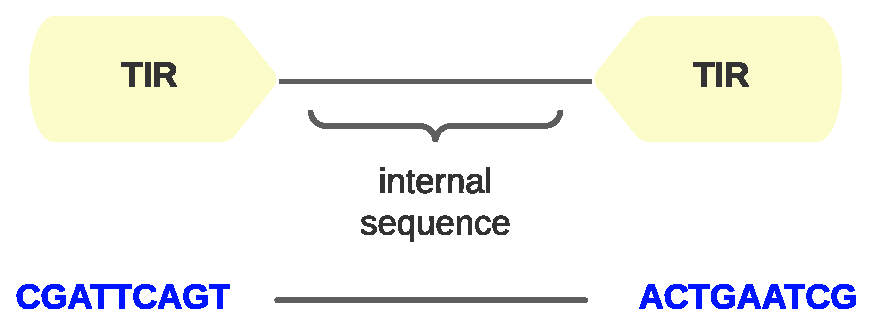
\includegraphics[width=0.6\textwidth]{img/misc/TIR.eps}
%        \caption{Exemple de \acrshort{tir}.}
%        \label{fig:TIR_exemple}
%    \end{figure}
    
%    \bigskip
    
%    \item[\ding{42}] \acrfull{ltr}: c'est une paire de séquences d'ADN identiques, qui peuvent avoir une longueur jusqu'à quelques centaines de nucléotides. Dans les rétrotransposons (Classe I) à \acrshort{ltr}, ces deux séquences se trouvent aux extrémités 5' et 3' de la séquence. \\
    
%    \bigskip
    
%    \begin{figure}[H]
%        \centering
%        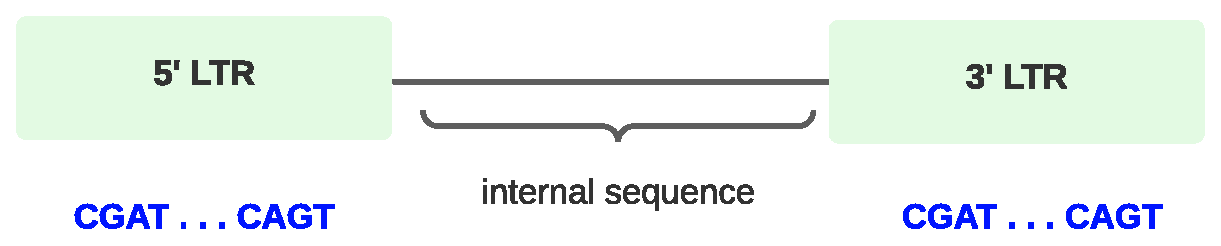
\includegraphics[width=0.7\textwidth]{img/misc/LTR.eps}
%        %\caption{Exemple de \acrshort{ltr}.}
%        %\label{fig:LTR_example}
%    \end{figure}
    
%    \bigskip
    
%    \item[\ding{42}] \acrfull{pbs}: il s'agit de la région nucléotidique où des amorces d'ADN peuvent venir se hybrider pour permettre à la réplication d'avoir lieu. Dans les \acrshort{et} du type \acrshort{ltr}, le \acrshort{pbs} a une taille qui est comprise entre 20 et 25 nucléotides, il est le complémentaire d'un \textit{tARN} et se trouve en 3', à quelque nucléotide près, du \acrshort{ltr} en 5'. Il est donc utilisé comme amorce pour la \acrfull{rt} \cite{wicker}. \\
    
%    \bigskip
    
%    \begin{figure}[H]
%        \centering
%        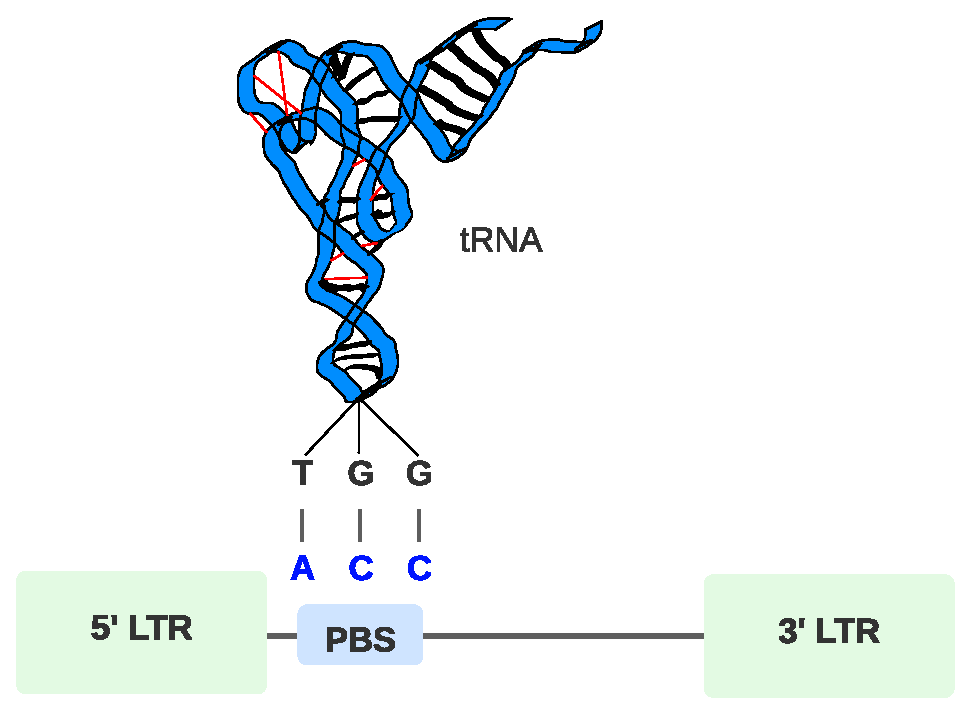
\includegraphics[width=0.6\textwidth]{img/misc/PBS.eps}
%        \caption{Exemple de \acrshort{pbs}.}
%        \label{fig:pbs_exemple}
%    \end{figure}
    
%    \bigskip
    
%    \item[\ding{42}] \acrfull{tsd}: il s'agit généralement d'une courte répétition directe qui est obtenue sur les régions flanquantes d'\acrshort{et} après son insertion. \\
    
%    \bigskip
    
%    \begin{figure}[H]
%        \centering
%        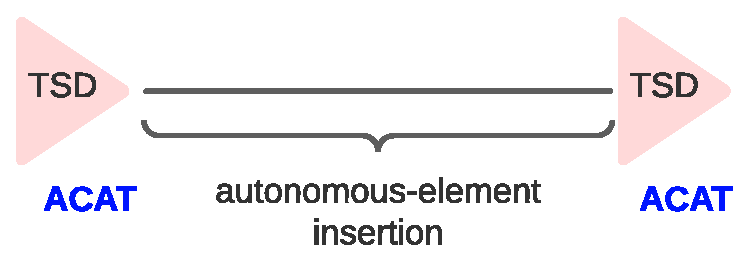
\includegraphics[width=0.6\textwidth]{img/misc/TSD.eps}
%        \caption{Exemple de \acrshort{tsd}.}
%        \label{fig:TSD_example}
%    \end{figure}
    
%\end{itemize}

%\newpage

\subsection{Contexte scientifique}\label{par:context}

\paragraph{Naissance de la question scientifique.} Le sujet de ce stage naît à partir d'un projet intitulé \textit{MosquiTEs} et coordonné par M. Boulesteix, lequel est aussi tuteur de ce stage. \\
Le projet vise à analyser le rôle des \acrlong{et} dans l'adaptation d'\textit{Ae. albopictus} dans des climats tempérés. \\
% , avec un regard central sur une possible influence/interférence de ceux-ci dans le processus de diapause 
% \footnote{Diapause: phase du développement de l'insecte pendant laquelle l'organisme devient inactif de manière volontaire pour arrêter sa croissance, de manger ainsi que de bouger. \\
% Ce ralentissement métabolique est généralement effectué par les insectes (mais aussi d'autres types d'animaux) pour survivre à des conditions environnementales défavorables ou alors pour dépasser des phases du développement qui sont particulièrement difficiles.
% } 
%de l'insecte. \\
La stratégie qui sera suivie dans le projet pour déterminer l'empreinte des \acrshort{et} dans l'adaptation est double: d'une part il y a le génotypage des nouvelles insertions d'\acrshort{et} de nombreux individus d'\textit{Ae. albopictus} (projet 1000 génomes); et d'autre part la caractérisation d'un point de vue moléculaire et macroscopique des phénotypes acquis grâce à ces insertions. \\

Dans ce stage, on s'intéresse principalement à l'annotation des \acrlong{et} sur le génome d'\textit{Ae. albopictus}. La librairie obtenue sera utilisée par la suite pour le génotypage. \\
Deux stratégies principales sont utilisées pour le génotypage: la méthode dite \acrfull{sr}, s'appuyant sur la propriété des lectures provenant d'une nouvelle insertion de chevaucher, d'une part une extrémité d'un élément annoté et de l'autre part le génome de référence et; la méthode dite \acrfull{drp}, laquelle se sert des lecture paired-end pour explorer un possible \acrfull{tip}. Par exemple, il explore deux lectures d'une paire ayant les extrémités s'alignant à des endroits différents, ou orientées de manière opposée ou encore si une seule des deux lecture s'aligne à la référence. \\
Il est donc d'importance capitale que les séquences d'\acrshort{et} contenues dans la librairie soient les plus complètes possibles, en particulier sur les extrémités, afin d'améliorer le résultat  du génotypage.
%et dans un deuxième temps à la mise en place des outils nécessaires pour le génotypage.

\newpage

\subsection{\'Etat de l'art}

% Comme anticipé, le travail réalisé est principalement divisé en deux étapes fondamentales:
% \begin{enumerate}
%     \item Annotation d'\acrlong{et} sur un assemblage du génome d'\textit{Ae. albopictus};
%     \item Préparation au génotypage sur le polymorphisme d'insertion de nouvelles copies (en anglais, \acrfull{tip}).
%     %sur les 56 génomes ci-dessus cités.
% \end{enumerate}

% \bigskip

\paragraph{Annotation des \acrshort{et}} La construction d'une librairie d'\acrlong{et} est une étape fondamentale pour l'annotation d'un nouveau assemblage d'un génome. La détection d'\acrshort{et} est généralement réalisée pour masquer les régions répétées du génome et permettre ainsi une meilleure annotation des éléments fonctionnels, comme les gènes. \\
Que ce soit pour cette dernière raison ou pour annoter réellement les \acrshort{et}, l'annotation des \acrshort{et} chez \textit{Ae. albopictus} a été déjà réalisée par plusieurs auteurs (\tableautorefname{ \ref{tab:annot_state_of_art}}). Le contenu d'\acrlong{et} chez \textit{Ae. albopictus} semblerait varier entre 40\% et 55\% en ayant une quantité plus ou moins équivalente selon l'annotation, de rétrotransposons et transposons à ADN.

\bigskip

\begin{table}[h]
    \centering
    \begin{tabular}{r|c|c|c}
        \toprule
         & \textbf{\makecell{\textit{Palatini et al}, \\ 2020}} & \textbf{\makecell{\textit{Melo et al}, \\ 2020}} & \textbf{\makecell{\textit{Goubert et al}, \\ 2015}}  \\
         \midrule
        \rowcolor{gray!10} 
        \textbf{Rétroéléments} & 22.69\% & 17.94\% & 17.67\% \\
        dont \acrshort{ltr} & 5.6\% & 7.84\% & 4.79\% \\
        \rowcolor{gray!10} 
        \textbf{Transposons à ADN} & 15.82\% & 7.4\% & 15.43\% \\
        \textbf{\makecell{Non classifiés et autres \\ éléments répétés}} & 17.3\% & 10.58\% & 16.63\% \\
        \midrule
        \rowcolor{gray!10} 
        \textbf{Total} & \textbf{55.81\%} & \textbf{43.76\%} & \textbf{49.73\% }\\
        \bottomrule
    \end{tabular}
    \caption{Composition en \acrlong{et} du génome d'\textit{Ae. albopictus} selon trois annotations différentes.}
    \label{tab:annot_state_of_art}
\end{table}

\bigskip

L'annotation réalisé par \textit{Goubert et al,} \cite{goubert_novo_2015} a été effectuée avec l'outil (\texttt{dnaPipeTE}) qu'ils ont proposé dans leur publication en utilisant des données \acrfull{shr}. L'annotation proposé par \textit{Melo et al,} \cite{melo_mosquito_2020} a été réalisé en utilisant un assemblage obtenu avec des lectures \acrshort{shr} \cite{chen_genome_2015} et le package \texttt{REPET} pour l'annotation. Enfin, la librairie proposée par \textit{Palatini et al,} \cite{palatini_improved_2020} a été réalisée avec leur assemblage obtenu à partir de données \acrfull{lr} (en utilisant \texttt{RepeatModeler}), mais n'a pas été rendue publique. \\

L'annotation d'\acrshort{et} peut être faite en utilisant trois types d'approches: par homologie (en utilisant une base de données d'\acrshort{et} et un assemblage), par \textit{de novo} en utilisant uniquement un assemblage et par \textit{de novo} mais en utilisant un génome séquencé (données brutes \acrfull{shr} ou \acrfull{lr}) \cite{goerner-potvin_computational_2018}. \\
Pour l'approche par homologie, l'outil qui actuellement représente le standard étant le plus utilisé au sein de la communauté, est \texttt{RepeatMasker} \cite{noauthor_repeatmasker_nodate}, lequel est majoritairement utilisé avec deux bases de données: \texttt{RepBase} \cite{jurka_repbase_2005} et \texttt{Dfam} \cite{storer_dfam_2021}. \texttt{RepBase} est réputée pour être la plus exhaustive; mais il existe aussi d'autres bases de données qui peuvent être spécifiques à un type d'élément (ex. \texttt{SINEBase}). \\ 


Pour l'approche \textit{de novo} en utilisant un assemblage, il existe une grande variété d'outils qui permettent l'annotation, mais deux se distinguent des autres par leur large utilisation au sein de la communauté: \texttt{RepeatModeler2} \cite{flynn_repeatmodeler2_2019} et \texttt{REPET} \cite{flutre_considering_2011}. Parmi les outils en utilisant des données de séquençage on retrouve \texttt{DNApipeTE} \cite{goubert_novo_2015}. On mentionne aussi \texttt{EDTA} \cite{ou_benchmarking_2019} qui est de plus en plus utilisé. \\
Ici de suite, on donne quelques détails concernant les outils d'annotation utilisés dans ce travail:

\begin{itemize}
    \item[\ding{42}] \texttt{RepeatMasker} est l'outil de référence pour l'annotation par homologie. Son fonctionnement consiste principalement à \og masquer \fg{} les séquences contenues dans la librairie fournie sur le génome analysé. Les séquences fournies comme base de données (ex. \texttt{RepBase} mais il peut également s'agir d'une librairie personnalisée) sont identifiées grâce un algorithme d'alignement local (\texttt{blastn} il en est un exemple).
    \item[\ding{42}] \texttt{RepeatModeler2} est un pipeline pour l'annotation automatique des \acrshort{et}. Il utilise quatre modules: \texttt{RECON} \cite{bao_automated_2002} et \texttt{RepeatScout} \cite{repeatscout} lesquels s'appuient sur la répétitivité des \acrshort{et} et, \texttt{LTRharvest} \cite{ellinghaus_ltrharvest_2008} et \texttt{LTR\_retriever} \cite{ou_ltr_retriever_2018} lesquels s'appuient sur la structure caractéristique des rétrotransposons \acrshort{ltr}. \\
    \texttt{RepeatScout} est utilisé pour sa rapidité dans la découverte des familles les plus récentes et abondantes sur le génome. \texttt{RECON} utilise des matrices de substitution sophistiquées ainsi que des pénalités pour les gaps affinées, en lui permettant de détecter aussi les familles les plus anciennes. \\
    \texttt{LTRharvest} est donc utilisé pour la détection des éléments (grâce à la signature caractéristique des \acrshort{ltr}) et \texttt{LTR\_retriever} pour filtrer les faux positifs détecté par \texttt{LTRHarvest}.

    \item[\ding{42}] \texttt{EDTA} utilise plusieurs modules pour l'annotation: \texttt{LTRharvest}, \texttt{LTRfinder} \cite{xu_ltr_finder_2007},  \texttt{LTR\_retriever}, \texttt{GRF} \cite{shi_generic_2019}, \texttt{TIR-Learner} \cite{su_tir-learner_2019}, \texttt{HelitronScanner} \cite{xiong_helitronscanner_2014}, et aussi \texttt{RepeatModeler} qui est utilisé comme filtre. \\
L'idée à la base du pipeline est la suivante: d'abord il appelle les modules spécifiques à des caractéristiques (\acrshort{ltr}, \acrshort{tir}, etc) et puis il masque le génome de référence avec les séquences obtenues (c'est-à-dire que les séquences détectées dans les étapes précédentes sont marquées comme telles; généralement une séquence masquée est remplacée par des \og X \fg{} sur le génome de référence utilisé) et ensuite il utilise \texttt{RepeatModeler} pour détecter les non-\acrshort{ltr} et les éléments non classifiés.
\end{itemize}

\bigskip

\paragraph{Génome de référence} Comme vu dans le paragraphe précédent, l'assemblage du génome de l'espèce sur laquelle on souhaite travailler est un choix important, car la qualité de l'annotation des \acrlong{et} en dépend. \\
Pour \textit{Ae. albopictus}, 6 assemblages sont actuellement déposés sur le NCBI \cite{information_national_nodate} dont uniquement 3 génomes sont assemblés au niveau des scaffolds: \textit{Chen et al.} \cite{chen_genome_2015}, \textit{Palatini et al.} \cite{palatini_improved_2020} et \textit{Boyle et al.} \cite{boyle_linkage-based_2021}. \\

Les deux derniers, ont été obtenus en utilisant des données de séquençage de type \acrfull{lr}. Parmi les trois, celui de  \textit{Boyle et al.} est le plus récent et le moins fragmenté, (du coup d'une certaine manière c'est le meilleur assemblage) mais à la différence de l'assemblage de \textit{Palatini et al.}, il manque une fraction de 200 Mbp. \\
En contrepartie, le travail de \textit{Palatini et al.}, présente dans son assemblage de nombreux haplotigs
\footnote{Il s'agit de plusieurs contigs qui provenant d'haplotypes différents. En d'autres mots, un haplotig est la duplication d'un contig en raison de la nature hétérozygote du génome analysé (deux copies du même allèle).}
, lesquels faussent la taille estimée du génome, étant en désaccord avec l'estimation par cytométrie en flux ($\sim$2.5 Gbp contre 1.190–1.275 Gbp). Un tableau résumant ces trois assemblages est disponible dans le \autoref{tab:assembly_comparaison}.

\bigskip

\paragraph{Classification}

La classification est une étape indispensable pour connaître à quel groupe d'\acrlong{et} une séquence appartient (voir \figureautorefname{ \ref{fig:classif_et}}). \\
Comme pour l'annotation, plusieurs outils existent, mais une méthode précise et répandue au sein de la communauté n'est pas définie. Cependant, plusieurs critères sont souvent retrouvés dans la bibliographie et utilisés. En particulier, il est très commun de trouver des approches similaires à ce décrit dans \textit{Wicker et al,} 2007. Dans ce papier, ils proposent de réaliser la classification en plusieurs étapes. \\
La première étape consiste en une recherche par homologie des séquences putatives (préalablement identifiées avec l'annotation) contre une base de données d'\acrshort{et} d'acides nucléiques (ADN vs ADN) en utilisant un outil du type \texttt{blastn} et en filtrant les résultats selon la règle 80-80-80, pour pouvoir associer les séquences aux familles correspondantes (quand cela est possible). \\
La deuxième étape consiste toujours dans un approche par homologie, mais cette fois-ci contre une base de données contenant les séquences des domaines protéiques des \acrlong{et} (ex. \texttt{Pfam} ou \texttt{RepeatPeps.lib}, provenant de \texttt{RepeatMasker}) avec un outil comme \texttt{blastx} (ADN traduit vs protéine). Ici l'idée est que, une nouvelle famille d'\acrshort{et} (qui donc n'a pas eu une forte similarité contre la base de données nucléiques), devrait quand même avoir des fortes correspondances avec les domaines protéiques de toutes les autres familles faisant partie de la même super-famille, avec lesquelles elle partage les domaines protéiques. \\
Dans le cas où la recherche contre les domaines protéiques ne donne aucun résultat, cela pourrait signifier que la famille fait partie d'une super-famille (ou même d'une classe) inconnue ou, alternativement il pourrait s'agir d'un élément non-autonome \footnote{\acrshort{et} sans séquence codante fonctionnelle mais pouvant être mobilisé par l'intervention de protéines produites par d'autres \acrshort{et}.}. \\
Du coup, si les deux premières méthodes ne donnent pas de résultats, une recherche de motifs structuraux (comme \acrshort{tir}, \acrshort{pbs}, \acrshort{tsd} ou encore \acrshort{ltr}; pour plus de détails, consulter le \textsc{\ref{sec:gloss}}) peut être réalisée. \\
Si les étapes précédentes échouent à donner un résultat satisfaisant pour la classification, la séquence est généralement marquée comme non-classifiée (\textit{Unknown}).


%TODO: peut-être qu'il faudra effacer ce paragraphe
%\paragraph{Génotypage de nouvelles copies d'\acrshort{et}} Dans la suite du projet, il est prévu de réaliser un génotypage des nouvelles insertions des \acrshort{et} sur 1000 génomes. Comme pour l'annotation, les outils candidats pour cette tâches, peuvent être subdivisés en plusieurs catégories selon le type de données utilisé, le type d'\acrlong{et} à détecter ou encore le type d'algorithme utilisé \cite{goerner-potvin_computational_2018}. \\

%Même si la plupart des outils peut être utilisé avec n'importe quel type de données, cela n'empêche pas le fait que qu'ils ont été conçus par un type particulière: \acrfull{shr} provenant d'une lignée germinale, \acrshort{shr} d'un pool d'individus, \acrshort{shr} provenant d'un seul individu, \acrshort{shr} provenant d'une lignée somatique ou encore pour des  \acrfull{lr}. \\
%Comme anticipé, ils existent plusieurs type d'algorithmes, lesquels se basent sur des stratégies différentes. La méthode dite \acrfull{sr}, s'appuie sur la propriété des lectures provenant d'une nouvelle insertion de chevaucher d'une part une extrémité d'un élément annoté et de l'autre part le génome de référence. \\
%La méthode dite \acrfull{drp} se sert des lecture paired-end pour explorer un possible \acrshort{tip}; par exemple si les extrémités des deux lectures s'alignent à des endroits différents, si elles sont  orientées de manière opposée ou si une seule des deux s'aligne à la référence. \\
%Une dernière stratégie consiste dans la recherche de motifs caractéristiques des \acrshort{et} directement dans les lectures. \\

%Dans \textit{Vendrell-Mir et al.} (2019) \cite{vendrell-mir_benchmark_2019}, les auteurs ont réalisé un benchmark de plusieurs outils. Notamment ils suggèrent \texttt{Trackposon} \cite{carpentier_retrotranspositional_2019} et \texttt{MELT} \cite{gardner_mobile_2017} pour leurs rapidité et précision; en effet ils sont conçus pour effectuer une recherche famille-spécifique et ils sont si rapide qu'ils ont déjà été utilisé dans le cadre de projets 1000 génomes. Pour une recherche étendue à tout type de famille de \acrshort{tip}, ils conseillent \texttt{PopoolationTE2} \cite{kofler_popoolationte2_2016} et en plus ils suggèrent son utilisation en combinaison avec d'autre outils comme \texttt{Jitterburg} \cite{henaff_jitterbug_2015} ou \texttt{TEFLoN} \cite{adrion_genome-wide_2017} pour une meilleure sensibilité et spécificité.

\newpage

\section{Matériel et méthodes}

\bigskip

\begin{figure}[H]
    \centering
    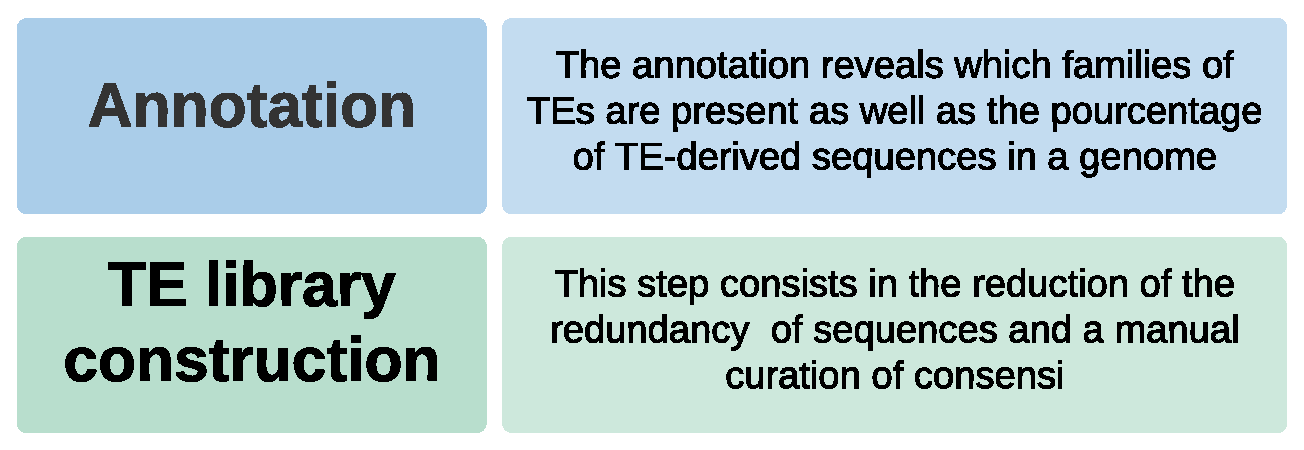
\includegraphics[width=0.7\textwidth]{img/misc/main_steps.eps}
    \caption{\'Etapes principales.}
    \label{fig:main_steps}
\end{figure}

\bigskip

En \figureautorefname{ \ref{fig:main_steps}} on retrouve les étapes qui ont été abordées au cours du projet. La première étape consiste dans la réalisation d'une nouvelle \textbf{annotation} des \acrlong{et} pour pouvoir obtenir des séquences candidates qui seront traitées dans la deuxième étape, la \textbf{construction de la librairie}. \\
La librairie produite sera utilisée pour effectuer le \textbf{génotypage} de nouvelles insertions (\og TE insertion calling \fg{}) dans le projet \textit{1000 génomes}. 
%Dans le cadre du stage, on a uniquement mis en place les outils nécessaires qui seront utilisés dans cet effet, mais l'argument ne sera pas traité dans ce document.

\subsection{Annotation}

Pour annoter les familles d'\acrshort{et} présentes dans le génome de référence on utilise un mélange de deux approches différentes et complémentaires : \textit{de novo} et par homologie. \\

\subsubsection{Approche \textit{de novo}}

Dans ce type d'approche, les \acrshort{et} sont identifiés grâce à les caractéristiques structurales qui sont spécifiques à chaque ordre (\acrshort{ltr}, \acrshort{tir}, etc) ainsi que grâce à leur nature répétée. \\
On a ainsi utilisé les programmes suivants sur le génome de référence: \\

\begin{itemize}
    \item[\ding{42}] \texttt{RepeatModeler2}: les commandes utilisées sont disponible dans le \autoref{RM2}. 
    \item[\ding{42}] \texttt{EDTA} \cite{ou_benchmarking_2019}: selon les instructions de l'auteur, on a séparés l'analyse en trois exécutions différentes, chacune pour un type d'\acrshort{et} différent (\texttt{helitron}, \texttt{\acrshort{tir}} et \texttt{\acrshort{ltr}}). Les commandes utilisées se trouvent ici : \autoref{edta}.
    \item[\ding{42}] \texttt{MITE-Tracker} \cite{crescente_mite_2018}: pour cet outil, il a été nécessaire de diviser le génome de référence en 11 fichiers plus petits pour limiter le temps de calcul, chaque fichier a été donc lancé avec l'option \texttt{-{}-task candidates}. Un dernier run avec l'option \texttt{-{}-task cluster} a permis de réunir les résultats obtenus (\autoref{mite}).
\end{itemize}

\paragraph{\'Evaluation des résultats}\label{par:eval} Pour évaluer les librairies obtenues avec les outils \textit{de novo}, on a effectué plusieurs types d'analyses: \\

\begin{itemize}
    \item[\ding{42}] Estimation de la redondance de chacune des librairies séparément (\subsectionautorefname{ \ref{par:redondance} - \textsc{\nameref{par:redondance}}}). Pour cela, on a réalisé un clustering de chacune des librairies à l'aide de \texttt{cd-hit-est} \cite{fu_cd-hit_2012} (\texttt{-c 0.8 -G 0 -aS 0.8 -d 0}). \\
    
    \item[\ding{42}] Exploration la distribution des longueurs des différents consensi (\subsectionautorefname{ \ref{par:lengths} - \textsc{\nameref{par:lengths}}}). Pour le faire, on a d'abord classifiées les séquences (de manière non définitive) avec \texttt{DeepTE} \cite{yan_deepte_2020} et ensuite on a comparé les longueurs de consensi issus \textit{de novo} avec ceux contenus en \texttt{RepBase}. \\ 
    
    \item[\ding{42}] Réalisation d'une estimation de la couverture génomique (\subsectionautorefname{ \ref{par:coverage} - \textsc{\nameref{par:coverage}}}). Pour faire cela, on a simulé des lectures \textit{Illumina} (au format \texttt{fastq}) à partir du génome de référence en utilisant \texttt{ART} \cite{huang_art_2012}, \texttt{samtools} \cite{danecek_twelve_2021} et \texttt{bedtools} \cite{quinlan_bedtools_2010} (\autoref{simulation}). Ensuite, on a utilisé le fichier obtenu pour estimer la couverture génomique par des éléments répétés en utilisant \texttt{dnaPipeTE} \cite{goubert_novo_2015} (\autoref{dnapipete}).
\end{itemize}


\subsubsection{Approche par homologie}\label{sec:homology}

Dans ce cas, les \acrshort{et} sont identifié par similarité avec des séquences d'\acrshort{et} précédemment annotés chez la même espèce ainsi que dans des espèces proches et, qui sont donc contenus dans une base de données. Ici nous avons choisi d'utiliser uniquement les séquences provenant d'\textit{Arthropodes} de la base de données \texttt{RepBase v25.08} (\textit{FASTA Edition}) \cite{jurka_repbase_2005}. On a donc utilisé les fichiers suivants (description des fichiers pourvu par les auteurs de \texttt{RepBase}): \\

\begin{itemize}
    \item[\ding{42}] \texttt{angrep.ref}: \acrshort{et} de l'espèce \textit{Anopheles gambiae};
    \item[\ding{42}] \texttt{drorep.ref}: \acrshort{et} de l'espèce \textit{Drosophila melanogaster};
    \item[\ding{42}] \texttt{invrep.ref}: \acrshort{et} d'autres espèces invertébrés;
    \item[\ding{42}] \texttt{invsub.ref}: \acrshort{et} de sous-familles d'invertébrés.
\end{itemize}


\subsubsection{Combinaison des deux approches}

La combinaison des deux approches permet d'obtenir un certain nombre de familles d'\acrshort{et} fiables grâce à l'annotation par homologie  mais également des possibles nouvelles familles grâce à l'approche \textit{de novo}. \\
On a donc concaténé les librairies générés par les outils \textit{de novo} avec le sous ensemble de \texttt{RepBase} pour affiner et construire une librairie (voir \subsectionautorefname{ \ref{subsec:lib_construction}}) propre d'\acrlong{et}.

\bigskip

\newpage

\subsection{Construction de la librairie d'\acrshort{et}}\label{subsec:lib_construction}

\bigskip

\begin{figure}[h]    
    \centering
    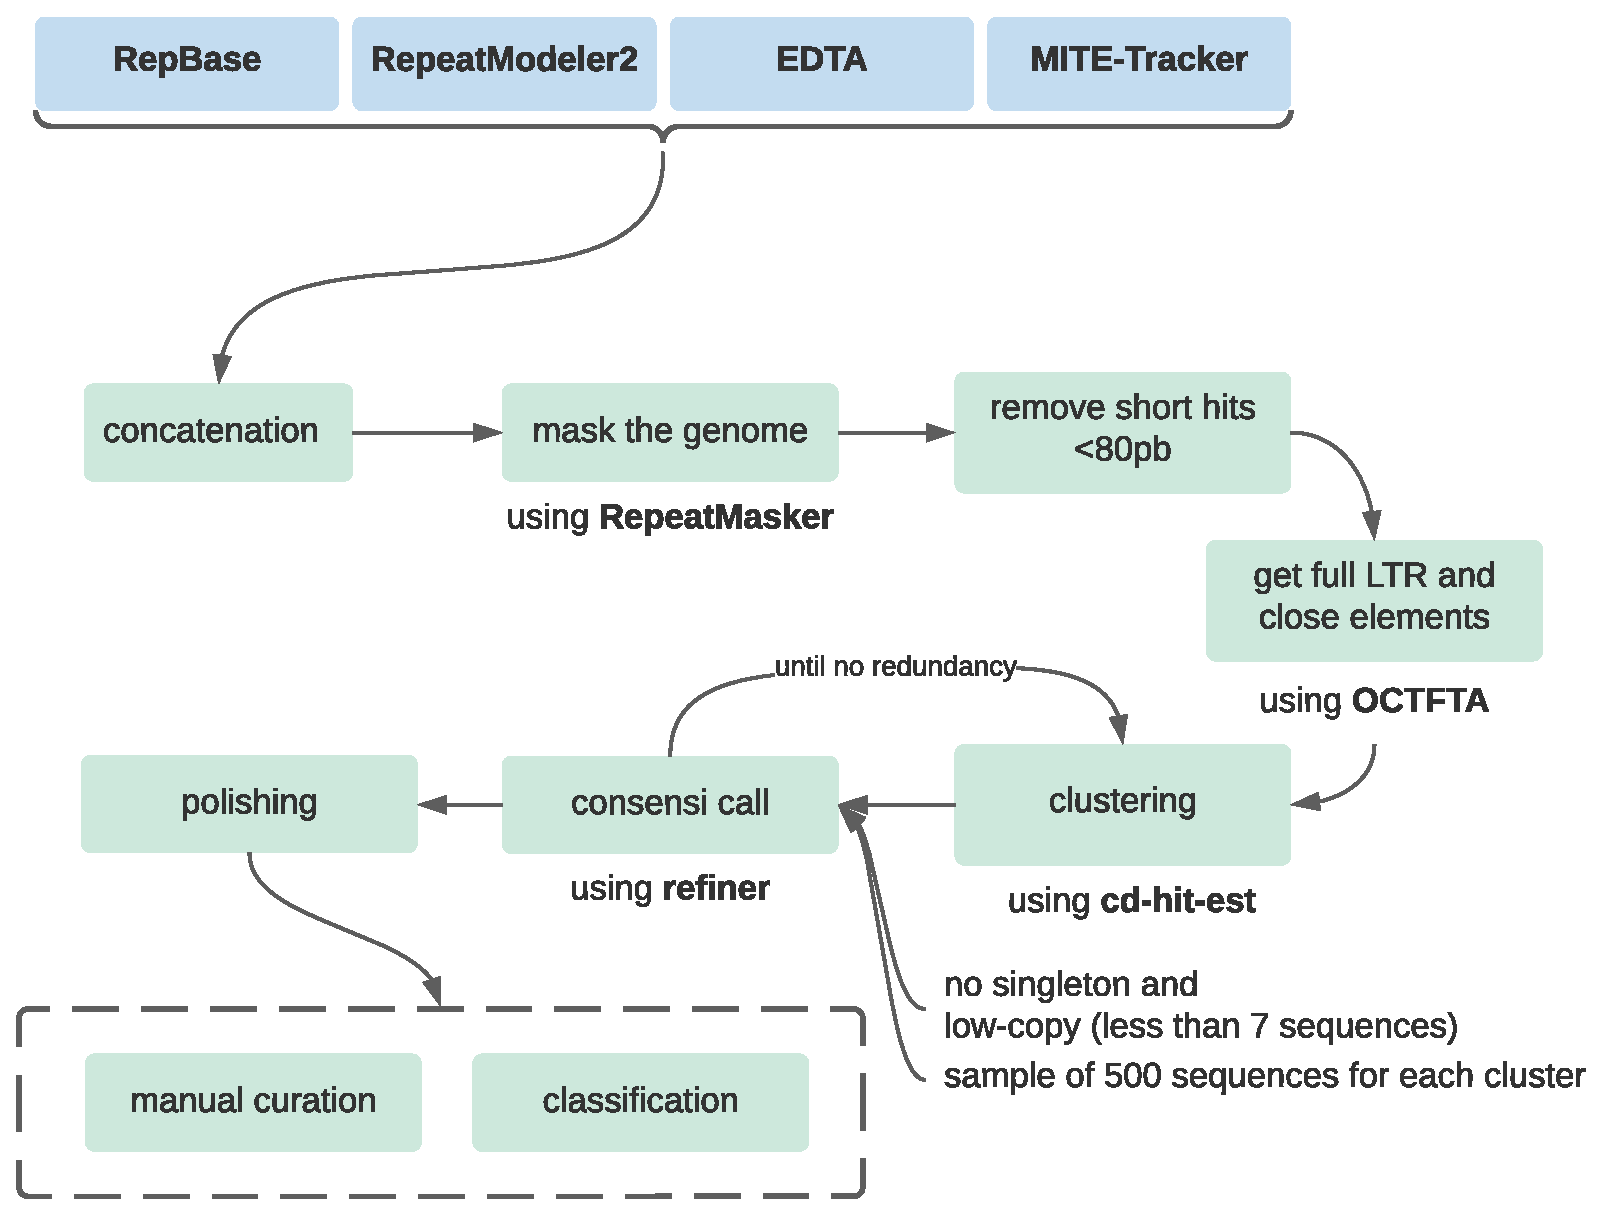
\includegraphics[width=0.9\textwidth]{img/misc/lib_construction.eps}
    \caption{Schéma des étapes suivies pour obtenir la librairie d'\acrshort{et}.}
    \label{fig:pipeline_lib}
\end{figure}

\bigskip

Pour obtenir la librairie d'\acrlong{et} on a suivi les étapes montrées sur la \figureautorefname{ \ref{fig:pipeline_lib}}. Pour commencer, on a concaténé les séquences obtenues avec les outils \textit{de novo} avec le sous-ensemble de \texttt{RepBase}. Dans la suite du document, on se référera à ce fichier avec le terme de libraire \og brute \fg{} ou \og concaténée \fg{}.\\
On a ensuite utilisé le fichier obtenu, comme librairie pour masquer le génome de référence en utilisant \texttt{RepeatMasker} \cite{noauthor_repeatmasker_nodate} (\autoref{repeatmasker}) avec la valeur de \texttt{-cutoff} la plus stringente possible (250), de manière à limiter le nombre d'éventuels faux positifs et, donc le nombre de séquences à traiter par la suite. \\
Outre que connaître la portion génomique représentée par des \acrshort{et}, l'outil permet de connaître aussi les positions de toutes les instances. \\
Pour mieux expliquer, une séquence dans la librairie utilisée (le fichier concaténé), représente une et une seule famille d'\acrshort{et} sous la forme d'un consensus
\footnote{
Une séquence consensus est une séquence qui contient les résidus les plus fréquents pour chacune des positions d'un ensemble de séquences. Dans notre cas, il s'agit d'une séquence \og moyenne \fg{} représentant une famille \acrshort{et}.
}. Or, en raison de leur nature répétée, les \acrshort{et} peuvent être présents en plusieurs copies à différents endroits du génome, étant chaque copie une instance (ou membre) de la famille. Dans le reste du document, \og consensus \fg{} et \og famille \fg{} indiqueront la même chose. De même, on pourra inter-changer les termes suivants: \og copie \fg{}, \og instance \fg{} ou encore \og membre \fg{}.\\ 
%\og fragment \fg{}. \\

En sortie de \texttt{RepeatMasker}, on a choisi d'éliminer les fragments ayant une longueur inférieure à 80 pb, pour performer ce filtrage, on a utilisé un script customisé (\linkautorefname{\ref{link1}}, se référer à la section \textsc{\ref{s:ext}}, dans les \textsc{\ref{s:annexes}}). \\

Les fragments restant ont été traités avec \texttt{\acrfull{octfta}} \cite{bailly-bechet_one_2014} pour reconstituer certaines copies entières. Pour clarifier, il n'est pas rare de trouver dans les bases de données, les \acrshort{ltr} et les régions codantes correspondantes (\figureautorefname{ \ref{fig:LTR_example}}) dans deux séquences séparées. Pour cette raison, \texttt{\acrshort{octfta}} permet de reconstituer les solo-\acrshort{ltr} avec leur élément interne (en se basant sur l'utilisation d'un préfixe commun pour la nomenclature du solo-\acrshort{ltr} et de son élément interne dans la base de données). \\
 De plus, la détection des \acrshort{et} avec \texttt{RepeatMasker} peut aussi retourner des copies fragmentées. Cela peut arriver si le score d'alignement entre le consensus en question et la région génomique analysée descend au-dessous d'un certain seuil entre différents portions du consensus. \\
\texttt{\acrshort{octfta}} permet également de fusionner deux fragments se trouvant en proximité sur le génome (\texttt{-{}-insert 80}, fusionnement de deux fragments si la distance entre eux est inférieur à 80pb).
Les commandes pour  \texttt{\acrshort{octfta}} se trouvent ici:\autoref{octfta}. \\
Un script customisé (\linkautorefname{\ref{link2}}) a été utilisé pour récupérer les séquences de toutes les copies (reconstituées ou pas) dans un seul fichier \texttt{FASTA}. \\

L'ensemble des copies a été utilisé ensuite pour un clustering avec \texttt{cd-hit-est} \cite{li_cd-hit_2006} (\autoref{cdhit}) pour réduire la redondance et pour regrouper les différentes instances provenant d'une même famille ensemble en essayant de respecter les conditions de la règle 80-80-80 (décrite ici: \paragraphautorefname{ \ref{par:explanation_te} - \textsc{\nameref{par:explanation_te}}}). Puis, en utilisant un script customisé (\linkautorefname{\ref{link2}}), on a séparé les clusters \textit{singleton} (ayant une seule séquence) et \textit{low copy} (ayant 6 ou moins séquences) dans deux fichiers séparés et sur les clusters restant on a utilisé \texttt{Refiner} (du package \texttt{RepeatModeler2}) pour appeler une séquence consensus à partir d'un échantillonnage de 500 séquences par cluster. \\
Par la suite, on a réalisé plusieurs cycles \texttt{cd-hit-est}/\texttt{refiner} pour réduire un maximum la redondance. \\

\subsubsection{Polissage}\label{sec:polish}

Chaque séquence a été ensuite polie avec un pipeline customisé (\linkautorefname{\ref{link4}}) pour essayer d'étendre les consensi, quand cela était possible, en vue du génotypage (comme expliqué dans le \paragraphautorefname{ \ref{par:context} - \textsc{\nameref{par:context}}}). Un schéma explicatif du pipeline est montré en \figureautorefname{ \ref{fig:polishte}}. \\
Brièvement, le pipeline prend en entrée une séquence putative d'élément transposable et le génome de référence utilisé pour l'annotation et il retourne la séquence polie. \\
Plus en détail: pour commencer il effectue un \texttt{blastn} \cite{camacho_blast_2009} de la séquence sur le génome, si plusieurs hits proviennent d'un même endroit génomique la séquence est marquée comme un possible \acrfull{ssr} et le programme se termine. Dans le cas contraire, un échantillonnage aléatoire des hits est effectué (par défaut, récupération de 100 hits dont 25 les plus longs) si nécessaire (prendre en compte tous les hits est extrêmement coûteux en termes de calcul). Ensuite les séquences associées sont extraites avec 1000pb flanquantes (100pb si la séquence de départ fait moins de 1Kb) de plus pour chaque extrémité en utilisant \texttt{bedtool slop}. Ces séquences sont donc alignées en utilisant \texttt{mafft} \cite{katoh_mafft_2002} et l'alignement obtenu est nettoyé à l'aide de \texttt{CIAlign} \cite{tumescheit_cialign_2022}. Cet outil permet notamment d'éliminer les \og insertions \fg{} rares de l'alignement (si l'insertion est présente en moins de la moitié des séquences formant l'alignement).  \\
\`A partir de l'alignement, un nouveau consensus est appelé et, si celui-ci est très similaire au consensus de départ et que les extrémités sont suffisamment couvertes par des hits, le pipeline se termine en retournant la nouveau consensus obtenu. \\
En revanche, si le consensus est suffisamment différent, une analyse sur la couverture des extrémités est effectuée: si elles sont très couvertes cela signifie que le consensus peut encore s'étendre donc on récupère des nucléotides supplémentaires aux extrémités, en revanche si elles ne sont pas couvertes cela signifie que probablement on a atteint la fin du consensus et qu'il faut donc tronquer les bases en excès récupéré avec l'extension précédente. La séquence obtenue est donc utilisée dans un nouveau cycle \texttt{blastn}-\texttt{mafft}-\texttt{CIAlign} et, le nouveau consensus est comparé à celui obtenu à l'itération précédente. \\
Lorsque la séquence d'une nouvelle itération est similaire à celle de l'itération précédente, cela signifie que le consensus a fini d'évoluer, donc le programme se termine et la dernière séquence est retournée. \\

\bigskip

\begin{figure}[H]
    \centering
    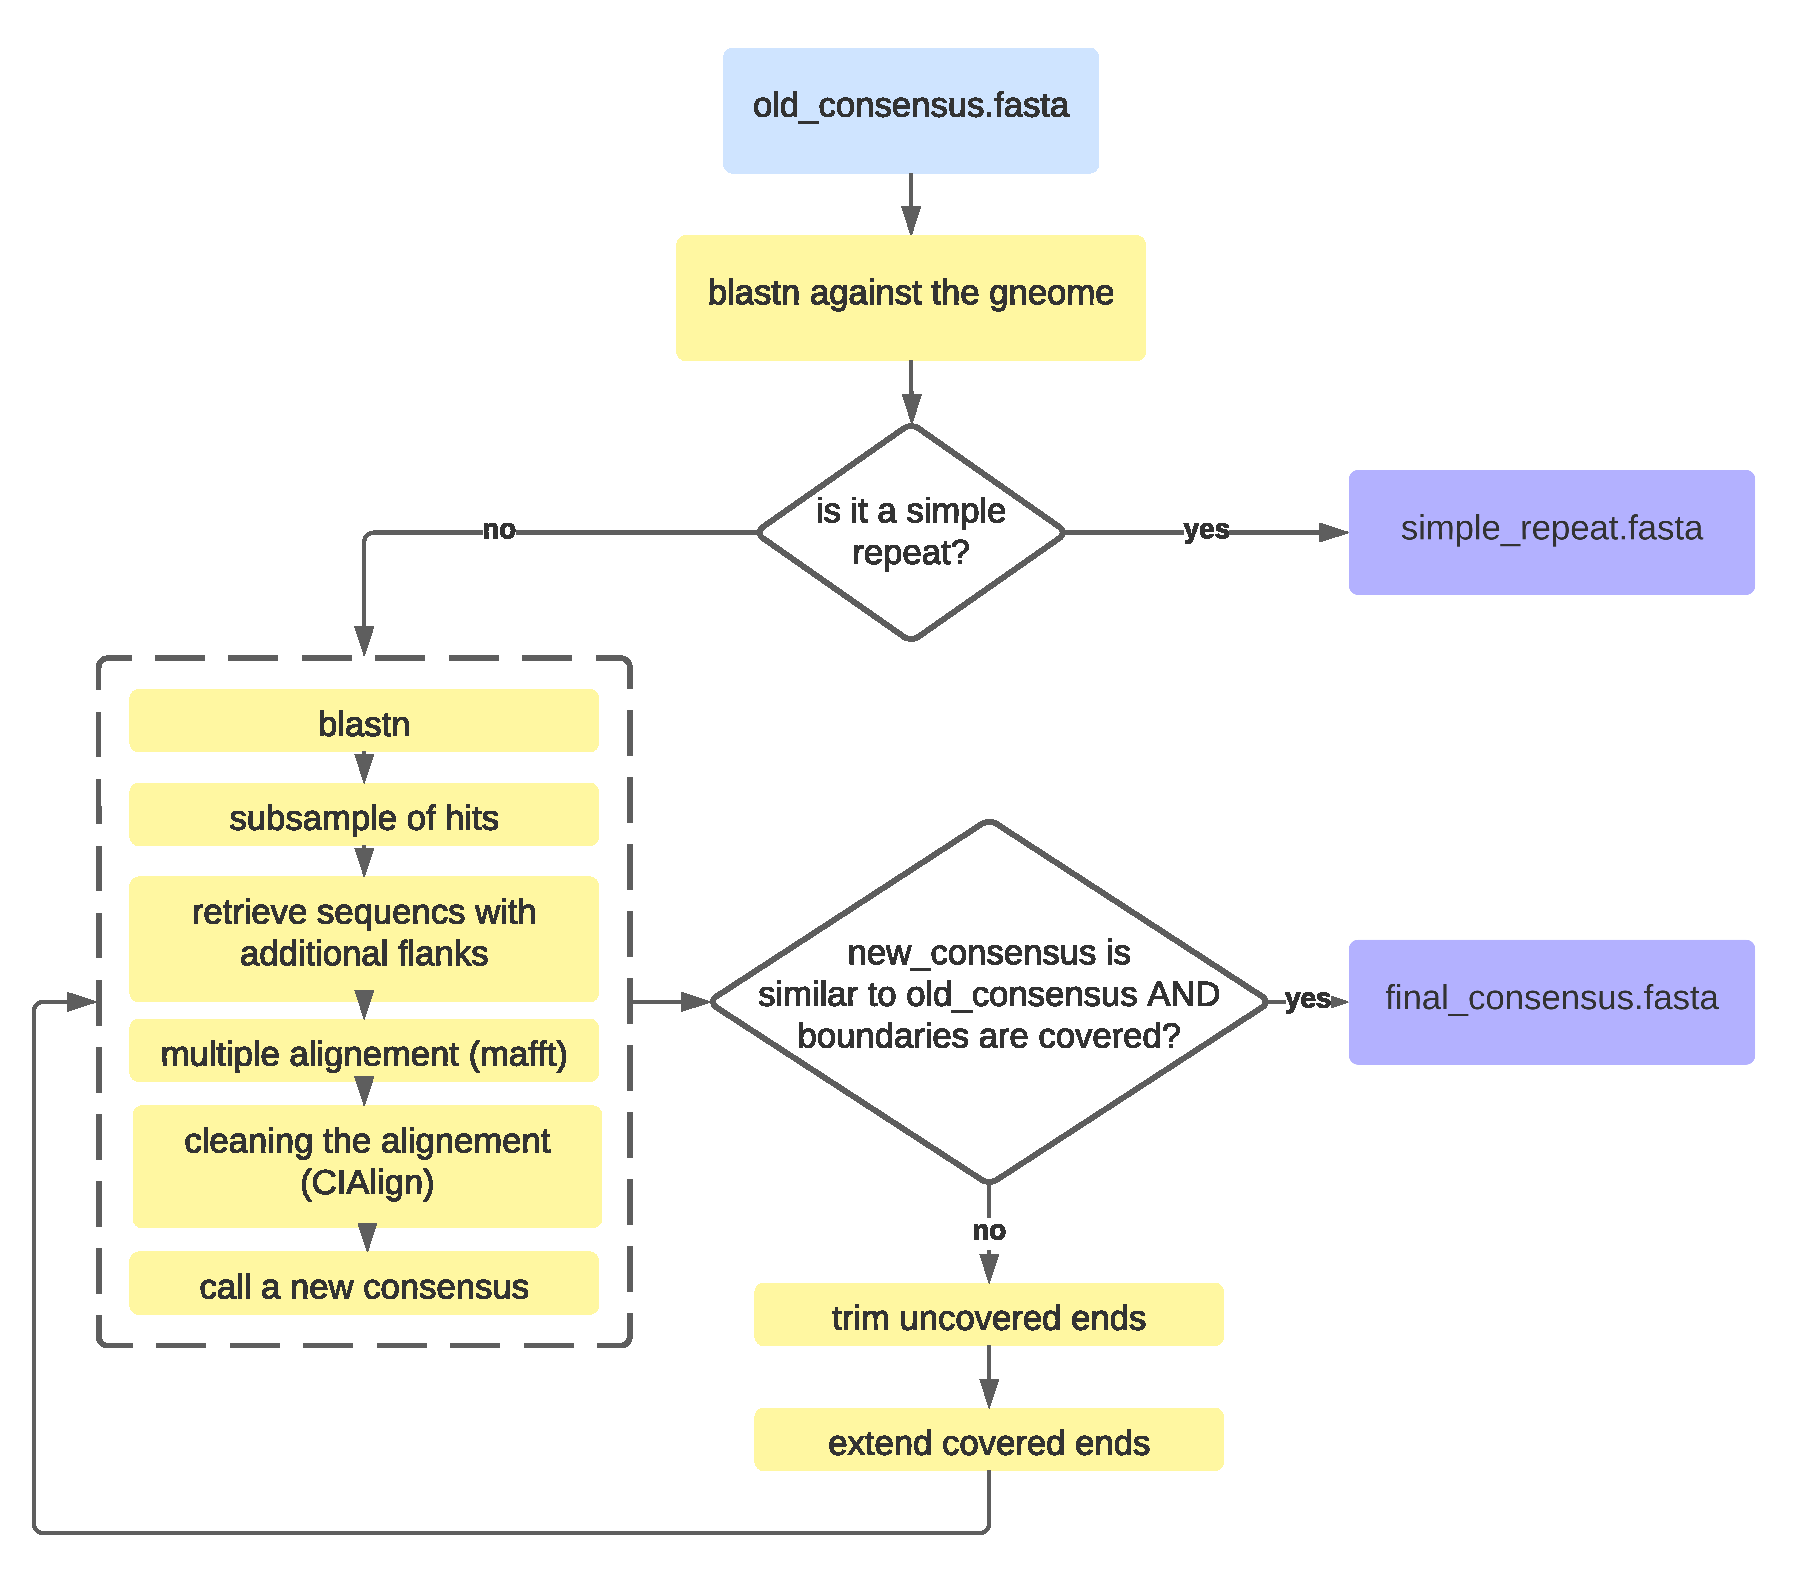
\includegraphics[width=0.9\textwidth]{img/misc/polishte.eps}
    \caption{Schéma explicatif du fonctionnement du programme pour le polissage des extrémités.}
    \label{fig:polishte}
\end{figure}

\bigskip

Le pipeline a été exécuté sur la totalité des séquences issues de l'étape de clutering, avec l'option \texttt{-ins 400} (permettant d'enlever les insertions rares dans l'alignement multiple issu de \texttt{mafft} jusqu'à une taille de 400pb, \autoref{polishte_code}). Les séquences marquées comme \acrshort{ssr} ont été mises de côté.

\subsubsection{Classification}\label{sec:classif_sec}

L'ensemble des séquences a été classifié en suivant les étapes montrées en \figureautorefname{ \ref{fig:classif}}. On a exécuté \texttt{RepeatMasker} (\texttt{-s -a -inv -nolow}) avec \texttt{RepBase27.03} sur notre librairie de séquences putatives. Ici, l'outil est utilisé dans le but de performer une recherche par homologie d'ADN contre ADN. \\
Le résultat a été filtré de manière à respecter la règle 80-80-80 (\autoref{rmout_filter}); ensuite le meilleur hit de chaque séquence a été choisi (en fonction du score d'alignement) (\linkautorefname{\ref{link5}}) et le fichier obtenu a été traité pour attribuer des super-familles (correspondantes aux familles identifiés) à chaque séquence (\linkautorefname{\ref{link6}}). En parallèle, on a utilisé \texttt{RepeatClassifier} (de la suite \texttt{RepeatModeler2}, outil qui utilise une recherche par homologie d'ADN sur de l'ADN et d'ADN traduit sur des protéines) et \texttt{RepeatProteinMask} (de la suite \texttt{RepeatMasker}, qui utilise aussi une recherche par homologie d'ADN traduit sur des protéines). Pour ce dernier on a filtré les hits en fonction d'un score minimum (>200) et d'une longueur minimale (au moins 80pb sur la séquence query) (\autoref{rmprot_filter}) et ensuite on a gardé que le meilleur hit (en fonction du score) pour chaque séquence (\linkautorefname{\ref{link5}}). \\
Une séquence a été classifiée si et seulement si le même résultat a été obtenu avec au moins deux outils sur trois (\linkautorefname{\ref{link7}}) dans un premier temps au niveau de la super-famille et ensuite (uniquement dans le cas où une super-famille a été identifiée), au niveau de la famille (quand possible). \\

\bigskip

\begin{figure}[H]
    \centering
    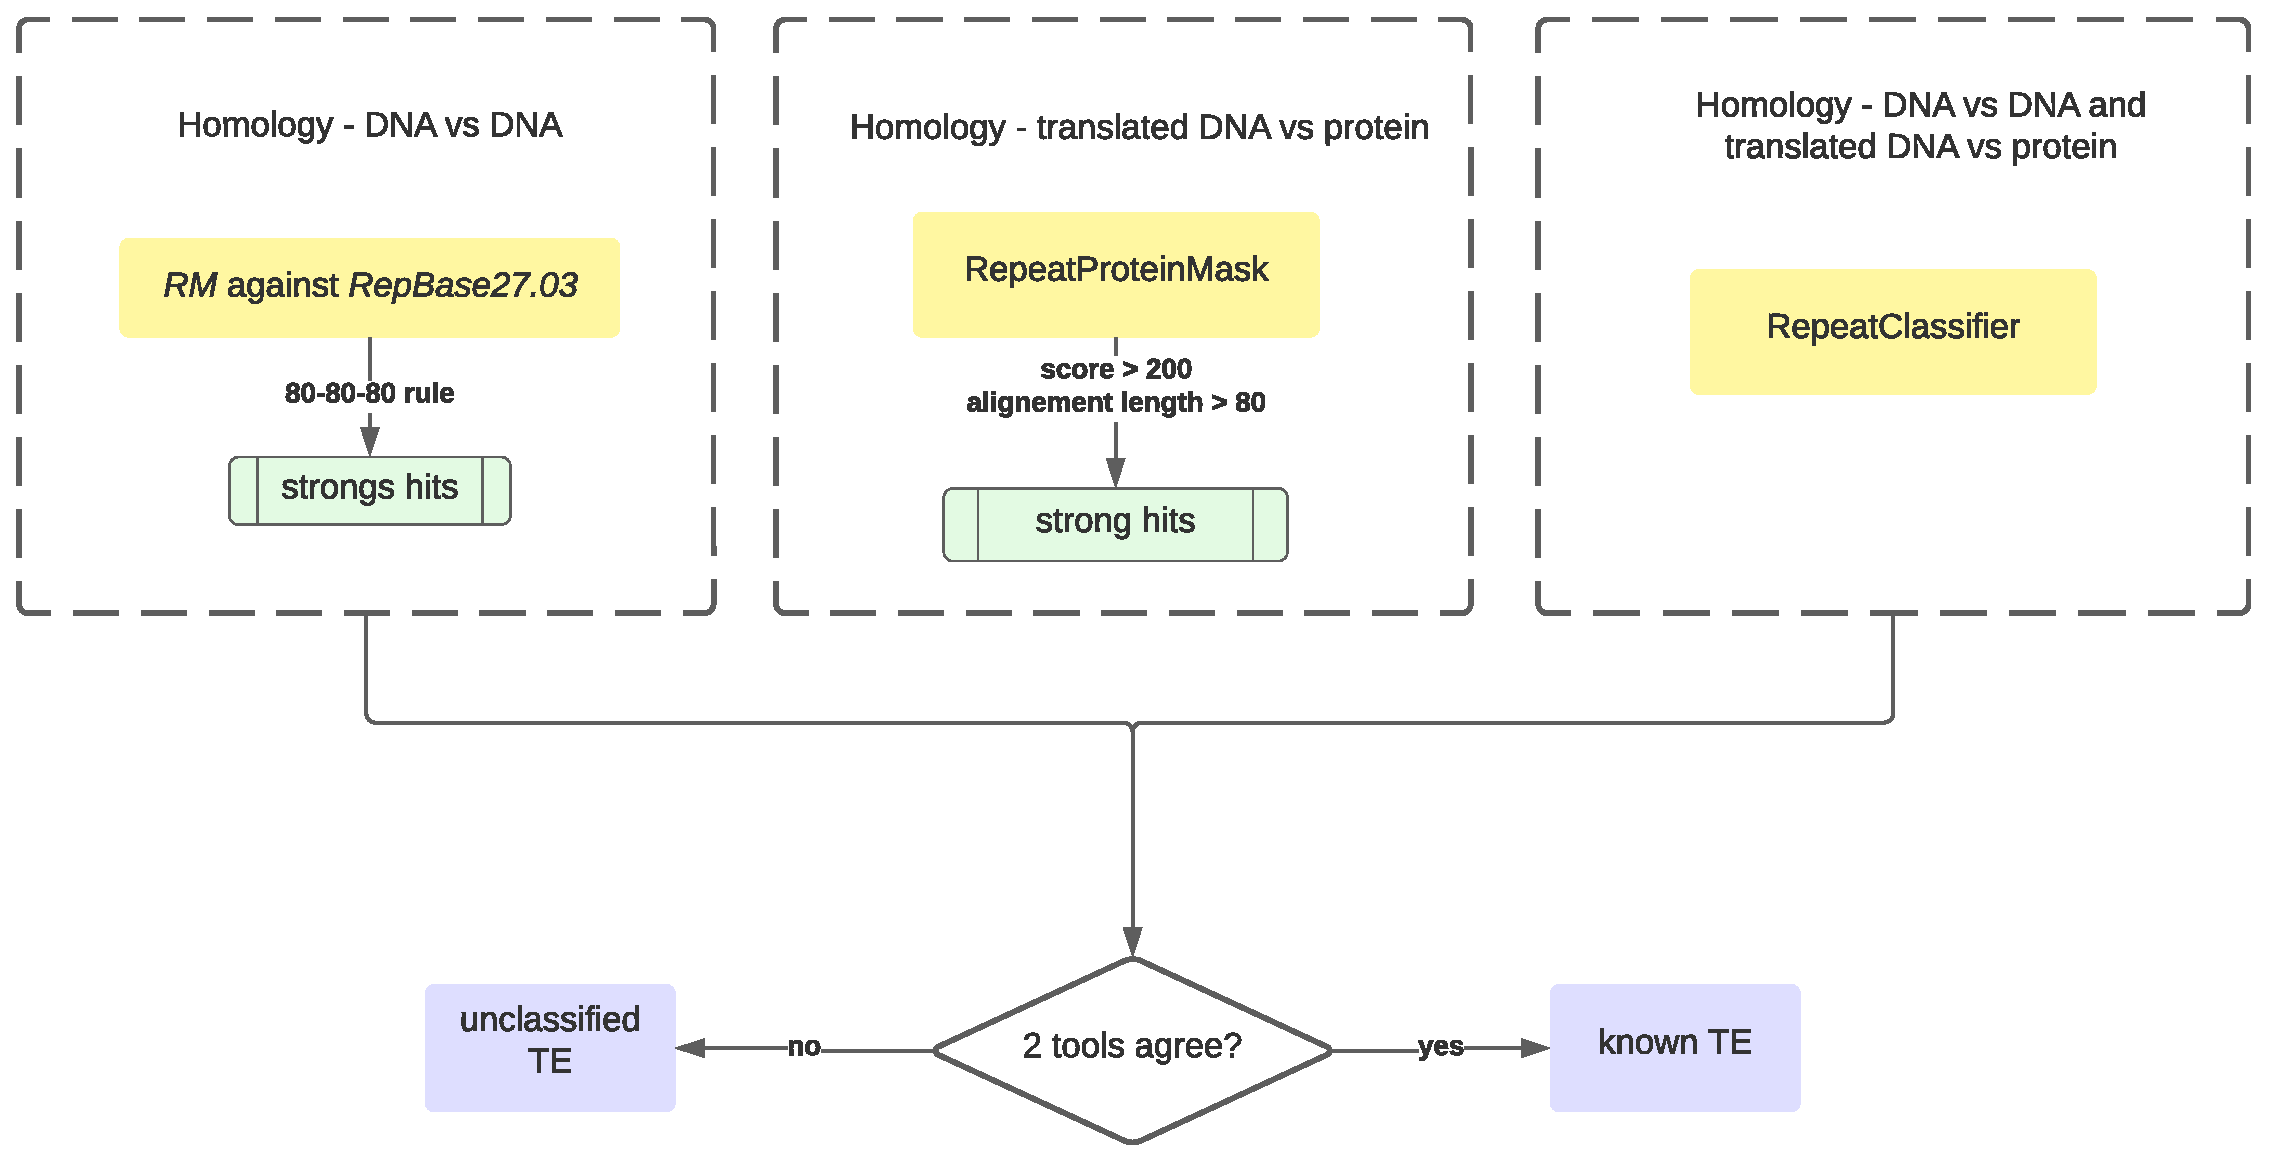
\includegraphics[width=0.9\textwidth]{img/misc/classif.eps}
    \caption{\'Etapes suivies pour la classification.}
    \label{fig:classif}
\end{figure}

\bigskip

Toute vérification manuelle des \acrshort{et}, à la fois pour le polissage et à la fois pour la classification, a été réalisé avec \texttt{TE-Aid} \cite{goubert_beginners_2022}.
%Sur les séquences non identifiées on a utilisé \texttt{einverted} \cite{rice_emboss_2000} pour détecter des éventuels \acrfull{tir}. Le fichier de sortie a été filtré de façon à garder que les séquences ayant une répétition inversée dans les premières 100pb. Ensuite, en fonction de la taille de la séquence, on a divisé les séquences (\href{https://github.com/TommasoBarberis/TE_Aalb/blob/main/scripts/library_construction/classification/tir_or_mite.py}{link}) en \acrshort{mite} (<650pb, car séquences trop courtes pour posséder des domaines protéiques) et \acrshort{tir} (>750pb). \\
%Enfin, les 20 séquences les plus répétées et les 20 séquences masquant le plus de génome ont été sélectionnées et manuellement annotées en utilisant \texttt{TE-Aid}. 


\newpage


%TODO: voir s'il faut l'effacer
%\subsection{Génotypage}\label{sec:geno} 

%TODO: nouveau outil supplémentaire?
%Le génotypage d'insertions d'\acrlong{et} consiste à identifier toutes les nouvelles insertions sur un nouveau génome. \`A l'occasion, celui-ci sera réalisé sur des données \textit{short-reads} de \textit{1000 génomes} et en utilisant la librairie obtenue aux étapes précédentes. On a donc mis en place les outils qui seront nécessaires. \\
%L'outil qui a été choisi pour effectuer le génotypage est \texttt{PoPoolationTE2}, pour cela, on a réalisé un container \texttt{singularity} pour faire si que l'outil puisse être  à la fois, utilisé sur des centres de calculs où l'utilisateur ne possède pas les droits d'installation, et à la fois pour figer la version de \texttt{PoPoolationTE2} ainsi que la version de \texttt{java} nécessaire pour utiliser correctement l'outil.
%rajouter Trackposon

\newpage\clearpage

\section{Résultats obtenus et discussion}

\subsection{\'Evaluation de l'annotation} 

Tout comme pour les gènes, l'annotation d'\acrlong{et} utilise aussi un assemblage du génome de l'espèce étudiée comme point de départ. On a choisi d'utiliser comme génome de référence l'assemblage de \textit{Palatini et al., 2020} (\textsc{Aalbo\_primary.1}, \url{https://www.ncbi.nlm.nih.gov/assembly/GCF_006496715.1}) malgré la présence de nombreux haplotigs. L'utilisation des lectures \acrlong{lr} \textit{PacBio} ainsi que sa couverture génomique \footnote{Fraction du génome couverte par l'assemblage.} font de lui le candidat préconisé pour cette tâche, avec 2 197 scaffolds et un N50 corrélé de 55 702 539. \\ 

Pour l'annotation \textit{de novo}, on a choisi d'utiliser d'un côté deux outils génériques pour maximiser la détection d'\acrshort{et}, \texttt{RepeatModeler2} et \texttt{EDTA}, et de l'autre un outil \acrshort{et}-spécifique, \texttt{MITE-Tracker}, car les \textit{\acrshort{mite}}, ont été trouvés en quantité significative dans l'annotation de \textit{Goubert et al,} 2015.

\paragraph{Résultats pour les outils d'annotation} \texttt{RepeatModeler2}, \texttt{EDTA} et \texttt{MITE-Tracker}, pour leur caractéristiques spécifiques ont généré des librairies différentes. Pour les explorer, on a utilisé \texttt{RepeatMasker} sur chacune de celles-ci.
% ainsi que sur \texttt{RepBase} (sous-ensemble décrit en \sectionautorefname{ \ref{sec:homology}}).

\bigskip

\begin{table}[h]
    \centering
    \rowcolors{4}{gray!10}{}
    \begin{tabular}{c|*5c}
        \toprule
        & & \textbf{\%} & \textbf{\%} & \textbf{\%} & \textbf{\%} \\
\textbf{Librairie} & \textbf{N.°}  & \textbf{génome} & \textbf{Classe I} & \textbf{Classe II} & \textbf{Non} \\    
        \textbf{utilisée}   & \textbf{séquences} & \textbf{masqué} & (dont \acrshort{ltr}) & & \textbf{classifiés} \\
        \midrule
        % \texttt{RepBase} & 17 410 & 38.28 & - & - & 38.28 \\
        \texttt{EDTA} & 16 191 & 77.53 & 37.94 (37.94) & 38.35 & 1.23 \\
        \texttt{RepeatModeler2} & 15 384 & 77.41 & 45.70 (30.78) & 9.75 & 18.15 \\
        \texttt{MITE-Tracker} & 10 863 & 31.33 & - & 31.33 & - \\
        \bottomrule
    \end{tabular}
    % \begin{tabular}{c|l}
    %     \textbf{\hspace{0.7cm} Total \hspace{0.7cm}} & \hspace{0.2cm}\textbf{59 848}\hspace{0.2cm} \\
    %     \bottomrule
    % \end{tabular}
    \caption{Nombre de consensi et pourcentage des classes (selon la classification effectué par l'outil considéré) pour les outils d'annotation utilisés.}
    \caption*{
    \scriptsize{
    \textbf{\% génome masqué}: représente le pourcentage du génome couvert par la librairie utilisée; 
    % (\texttt{RepBase} ou les librairies obtenues avec les outils \textit{de novo}); 
    \textbf{\% Classe I}: pourcentage de rétrotransposons;
    % valeur pour \texttt{RepBase} absente car la version utilisée n'était pas formatée pour être utilisée avec \texttt{RepeatMasker}, 
    % pour \texttt{MITE-Tracker} c'est logique de ne retrouver pas des rétrotransposons; 
    \textbf{\% Classe II}: pourcentage d'\acrlong{et} à ADN;
    %pour \texttt{RepBase} il y pas de valuer pour la même raison que les classe I; 
    \textbf{\% Non classifiés}: pourcentage d'éléments n'ayant pas reçu de classification.
    }
    }
    \label{tab:results_annotation}
\end{table}

\bigskip

Dans le \tableautorefname{ \ref{tab:results_annotation}} on peut observer les tailles des librairies obtenues ainsi que les pourcentages du génome qu'elles permettent de masquer. \texttt{EDTA} et \texttt{RepeatModeler2}, lesquels sont deux outils de détection famille non-spécifique, ont détecté
presque deux fois plus que dans l'annotation de \textit{Melo et al.} \cite{melo_mosquito_2020} (\tableautorefname{ \ref{tab:annot_state_of_art}}). \\
% d'éléments que l'approche par homologie (respectivement 77.53\% et 77.41\% contre le 38.28\% avec \texttt{RepBase}). \\
Globalement, les outils \textit{de novo} semblent être capable de détecter des nouvelles familles d'éléments, vu la large portion de génome couverte, mais par exemple, si on tient compte du pourcentage du génome masqué avec la librairie obtenue avec \texttt{MITE-Tracker}, on se rend compte qu'on devrait s'y attendre à avoir un tiers du génome occupé par des \textit{\acrshort{mite}}. Cela semblerait être improbable (par exemple, dans \textit{Goubert et al.}, le pourcentage de \acrshort{mite} a été estimé à 6.04\% du génome) et ça nous laisse penser que les outils \textit{de novo} peuvent avoir un fort taux de faux positifs. \\
D'ailleurs, le nombre de consensi obtenu pour chaque librairie \textit{de novo} n'est pas anodin, il suffit de penser que dans l'annotation de \textit{Goubert et al,} ils ont identifié 5 141 séquences consensus au total. On peut donc facilement suspecter une forte redondance dans les résultats ces outils. \\

\subsubsection{\'Evaluation de l'annotation \textit{de novo}}

\paragraph{\'Evaluation de la redondance des différentes librairies}\label{par:redondance}
%TODO: add ref to méthod&mat, reprendre le paragraphe
On a ainsi choisi de clusteriser chaque librairie \textit{de novo} (voir \sectionautorefname{ \ref{par:eval} - \textsc{\nameref{par:eval}}}) séparément. Les résultats sont montré dans la \autoref{tab:redondant_consensi}. \\
%Une séquence a été considéré comme redondante si et seulement si elle avait 100\% d'identité sur la totalité de la longueur avec un autre séquence. 
%Si on considère que chaque cluster obtenu représente une famille (en raison de la règle 80-80-80), 
On peut constater que \texttt{MITE-Tracker} passe de 10 863 consensi à 1 313 clusters (87,91\% familles en moins par rapport au nombre de départ); \texttt{RepeatModeler2} passe de 15 384 à 8 215 (46.60\% en moins) et \textit{EDTA} passe de 16 191 à 14 957 (réduction du nombre de famille uniquement du 7.62\%). Le fort taux de redondance pour \texttt{MITE-Tracker} pourrait être lié au fait qu'il a été utilisé sur 11 fichiers séparés (le génome a été découpé en plusieurs morceaux, pour permettre un temps de calcul raisonnable). \\
Ainsi, la librairie obtenue avec \texttt{MITE-Tracker} paraît être la plus redondante des trois tandis qu'\texttt{EDTA} est à l'apparence la moins redondante. \\
Une observation plus détaillée des clusters obtenus avec  \texttt{RepeatModeler2}, a permis de faire ressortir le fait que 6 263 séquences (soit le 40.71\% du nombre de départ de consensi) sont en fait des dupliqués, c'est-à-dire qu'elles sont 100\% identiques avec d'autres séquences déjà présentes dans la librairie. \\
Cela pourrait être dû au fait que \texttt{RepeatModeler2} a été exécuté en deux fois, avec le deuxième run en modalité \og \textit{recover} \fg{} (permettant de reprendre une exécution qui a été interrompue auparavant \footnote{
La premier exécution de \texttt{RepeatModeler2} a été interrompue pour permettre l'exécution du programme sur une plateforme plus adéquate.
}).


\bigskip

\begin{table}[h]
    \centering
    \begin{tabular}{r|c|c|c}
        \toprule
        \textbf{\makecell{Outil \\ d'annotation}} & \textbf{\makecell{Nb de séquences \\ de départ}} & \textbf{Nb de clusters} & \textbf{\makecell{Nb de séquences \\dupliquées}} \\
        \midrule
        \rowcolor{gray!10}
        \texttt{RepeatModeler2} &  15 384 & 8 215 & 6 263 \\
        \texttt{EDTA} & 16 191 & 14 957 & 0 \\
        \rowcolor{gray!10}
        \texttt{MITE-Tracker} & 10 863 & 1 313 & 0 \\
        \bottomrule
    \end{tabular}
    \caption{Nombre de séquences redondantes pour chaque librairie \textit{de novo}.}
    \caption*{
    \scriptsize{
    Le nombre de séquences de départ correspond au nombre de consensi contenu dans chacune des librairies obtenues par les outils \textit{de novo}. Chaque cluster regroupe plusieurs séquences, qui \textit{a priori} proviennent de la même famille d'\acrshort{et} (en raison de la règle 80-80-80 appliquée pour réaliser le clustering). 
    }
    }
    \label{tab:redondant_consensi}
\end{table}

\bigskip


\paragraph{\'Evaluation des distributions des longueurs}\label{par:lengths} Pour évaluer les consensi générés par ces outils, on a choisi de comparer la distribution des leurs longueurs avec celles de \texttt{RepBase}. Pour faire cela nous avons classifié les consensi en utilisant \texttt{DeepTE} \cite{yan_deepte_2020} pour avoir une information sur la classification des séquences. \\
On a choisi d'utiliser \texttt{DeepTE} pour son approche innovante (réseau neuronal convolutif) et sa rapidité, mais vu qu'il s'agit d'un outil encore peu utilisé au sein de la communauté, on a choisi de le tester. On a donc essayé de classifier les séquences contenues dans \texttt{RepBase} et de voir si le logiciel renvoyait la même classification que celle proposée dans la base de données (\linkautorefname{\ref{link8}}). Sur les 17 365 séquences classifiées, \texttt{DeepTE} a réussi en classifier correctement 9 356 (soit le 53.87\%) au niveau de la super-famille. \\
%Même si le résultat n'est pas excellent, on peut estimer que pour une classification au niveau au-dessus de la super-famille, donc au niveau de l'ordre, puisse être suffisant dans une analyse préliminaire comme celle-ci. \\

\begin{figure} 
    \centering
    \includegraphics[width=\textwidth]{img/plots/length_dist.eps}
    \caption{Distribution des longueurs des consensi identifiés par les outils \textit{de novo} et dans \texttt{RepBase}.}
    \caption*{\scriptsize
    Chaque sous-figure représente un type d'\acrshort{et} (\acrshort{ltr}, DNA, \acrshort{line}, \acrshort{sine}, non-\acrshort{ltr} et \acrshort{mite}). Sur l'axe de l'abscisse on retrouve les différents intervalles de longueur et sur l'axe des ordonnées le pourcentage des séquences contenues dans un intervalle donné pour un outil donné. Par exemple, environ le 50\% des séquences classifiées comme \acrshort{ltr} (par \texttt{DeepTE}) provenant de \texttt{RepeatModeler2}, sont contenues dans l'intervalle [0-1400]. 
    }
    \label{fig:dist_length}
\end{figure}

En \figureautorefname{ \ref{fig:dist_length}} (\linkautorefname{\ref{link9}}) on peut observer la distribution des longueurs pour les différents types d'\acrshort{et} (\textit{\acrshort{ltr}}, \textit{DNA}, \textit{\acrshort{line}}, \textit{\acrshort{sine}}, \textit{non-\acrshort{ltr}} et \textit{\acrshort{mite}}) pour les différents outils (\texttt{RepeatModeler2}, \texttt{EDTA} et \texttt{MITE-Tracker}) comparés aux séquences de \texttt{RepBase}. On a donc une sous-figure par type d'\acrshort{et}, sur l'axe des abscisses on retrouve les intervalles de longueurs et en ordonnées le pourcentage de séquences pour un outil donné et un intervalle donné. \\
Premièrement, on peut noter la difficulté de \texttt{DeepTE} à classifier correctement les \acrshort{mite}. On peut le constater par le fait qu'on a des séquences provenant de \texttt{MITE-Tracker} classifiées comme \acrshort{ltr}, \acrshort{line}, \acrshort{sine} et non-\acrshort{ltr}. Les \acrshort{mite} classifiés comme ADN sont moins problématiques, car dans la littérature ils sont souvent classifié comme des éléments non-autonomes de Classe II. \\
Il pourrait également s'agir de faux positif générés par \texttt{MITE-Tracker}, mais vu la longueur des ces séquences (les \acrshort{mite} sont connus pour être des séquences courtes, ayant moins de 800pb), un erreur dans la classification performée avec \texttt{DeepTE} paraît plus probable. \\
Sur une vue d'ensemble, on observe les mêmes distributions de longueurs que dans \texttt{RepBase} pour tous les outils et tous les types. Cependant, on peut remarquer que dans les intervalles ayant les longueurs les plus élevées (vers la droite), la librairie qui dans la plupart des cas possède le pourcentage le plus élévé, est \texttt{RepBase}. On peut voir cela dans les intervalles [2800-4200], [4200-5600] et [5600-7000] pour les \acrshort{ltr}; [2400-3200] et [3200-4000] pour les ADN; [3200-4800] et [4800-6400] pour les \acrshort{line}; [160-320], [320-480] et [480-640]  pour les \acrshort{sine}; [4200-5600] et [5600-7000] pour les non-\acrshort{ltr} et; [480-640] pour les \acrshort{mite}. \\
La majorité des consensi les plus longs proviennent de \texttt{RepBase}, ainsi il semblerait que les outils \textit{de novo} fournissent bien souvent des consensi tronqués, on montre donc encore plus le besoin d'étendre les séquences (\subsectionautorefname{  \textsc{\ref{sec:polish} - \nameref{sec:polish}}}) (spécialement pour celles issues d'un approche \textit{de novo}). \\

Pour les \textit{\acrshort{ltr}}, parmi les outils \textit{de novo}, \texttt{RepeatModeler2} est l'outil qui en détecte le plus (9 315 consensi). Pour les \textit{DNA}, c'est \texttt{EDTA} (3 803 consensi). \\
L'outil qui a détecté le plus de \textit{\acrshort{line}} et \textit{non-\acrshort{ltr}} est \texttt{EDTA} (respectivement 400 et 104 consensi) et, celui qui a annoté le plus de \textit{\acrshort{sine}} est \texttt{RepeatModeler2} (30 consensi). \\
Enfin, pour ce qui concerne les \textit{\acrshort{mite}}, on observe la quasi-absence de consensi en \texttt{RepBase} (uniquement deux séquences), ce qui nous permet de re-souligner l'importance d'utiliser un double approche \textit{de novo}/homologie. Sans surprise, l'outil qui a annoté le plus d'éléments est \texttt{MITE-Tracker} avec 7 770 consensi. \\

Globalement, les séquences pour les différentes types d'\acrshort{et} obtenues par les outils \textit{de novo} ont des longueurs similaires aux séquences contenues dans \texttt{RepBase}, donc on peut pas imaginer de filtrer des faux positifs parmi les consensi en fonction de ce critère. \\

\bigskip

\paragraph{\'Evaluation de la couverture génomique}\label{par:coverage}

Les librairies générées par les outils \textit{de novo} couvrent une large portion du génome, ce qui nous laisse penser à une possible présence de faux-positifs. Pour estimer la proportion d'éléments répétés, on a exécuté \texttt{dnaPipeTE} \cite{goubert_novo_2015} sur des données simulées à partir de l'assemblage (pour plus de détails, voir \paragraphautorefname{ \ref{par:eval} - \textsc{\nameref{par:eval}}}). \\

\bigskip

\begin{figure}[h]
    \centering
    \includegraphics[width=0.9\textwidth]{img/plots/coverage_simulated.eps}
    \caption{Estimation de la fraction répétée du génome d'\textit{Aedes albopictus}.}
    \caption*{\scriptsize
    %TODO: check la description du graphe avec Matthieu
    \textbf{A} - \textbf{Nombre des bases alignées par composante en fonction de la proportion génomique.} En rouge, la fraction génomique fortement répétée; en rose, la fraction normalement répétée et enfin, en vert l'ADN non répété. \textbf{B} - \textbf{Estimation de la composition en \acrlong{et}.}
    }
    \label{fig:coverage_simulated}
\end{figure}

\bigskip

En \figureautorefname{ \ref{fig:coverage_simulated}A}, on peut voir que l'outil identifie le 60.5\% du génome étant comme répété.
%(et $\sim$15\% comme fortement répété). \\
Par rapport aux résultats montré en \tableautorefname{ \ref{tab:results_annotation}}, il semblerait que \texttt{RepeatModeler2} et \texttt{EDTA} surestiment la fraction répétée du génome (respectivement de 17.03\% et 16.91\%). Il pourrait aussi s'agir d'une sous-estimation de \texttt{dnaPipeTE}, mais ses résultats sont plus en ligne avec les résultats précédemment obtenus (\tableautorefname{ \ref{tab:annot_state_of_art}}). \\
En \figureautorefname{ \ref{fig:coverage_simulated}B}, même si de manière approximative, on peut voir une nouvelle estimation des \acrlong{et} constituant la fraction répétée. On note principalement des \acrshort{line} (7.33\%), des ADN (4.21\%) (ainsi que des Helitrons, 2.14\%) et des \acrshort{ltr} (1.85\%). Cependant, la majorité reste non-classifié (37.97\%). \\


%Pour \texttt{MITE-Tracker}, ce genre d'évaluation est plus complexe, car les autres deux outils permettent une détection non-spécifique à une famille, tout comme \texttt{dnaPipeTE}. \\

On a également effectué un deuxième contrôle (\figureautorefname{ \ref{fig:repbase_realsize}}), en utilisant \texttt{RepBase} à la place de la librairie de défaut et sur un vrai jeu de données (\texttt{SRR10038864}) d'\textit{Ae. albopictus}, en utilisant comme paramètre pour la taille du génome, l'estimation par cytométrie en flux (1,23Gb). Le pourcentage obtenu pour la fraction répétée est de 59.4\%. Ce pourcentage est très similaire à celui obtenu sur les données simulées et au même temps il ne s'éloigne pas trop des annotations d'autres auteurs (\tableautorefname{ \ref{tab:annot_state_of_art}}), il permet donc d'avoir une idée de la vraie fraction répétée du génome. \\

\bigskip
% \newpage

\subsection{Construction de la librairie}

\subsubsection{Récupération des copies}\label{get_copies}

Après concaténation (\figureautorefname{ \ref{fig:pipeline_lib}}) des librairies brutes, la librairie fusionnée contient \textbf{59 848} séquences, dont 42 438 provenant des outils \textit{de novo} et 17 410 provenant de \texttt{RepBase}. \\
Après avoir utilisé \texttt{RepeatMasker} sur la librairie fusionnée, on obtient \textbf{8 966 074} séquences qui ont été masquées sur le génome, en couvrant 80.94\% de celui-ci. \\
Parmi les 59 848 consensi de départ, uniquement 38 165 (63.7\% de la librairie fusionnée) d'eux ont eu une correspondance sur le génome. \\
%Cela peut sembler étrange, car finalement les outils \textit{de novo} s'appuient sur le génome fourni pour générer les consensi, cependant il faut tenir compte des choses suivantes: \\

%\smallskip

%\begin{itemize}
 %   \item[\ding{42}] parmi les 59 848 consensi de départ il y en a beaucoup qui proviennent de \texttt{RepBase}, où plusieurs séquences proviennent d'espèces plus ou moins phylogénétiquement distantes;
  %  \item[\ding{42}] le clustering réalisé et montré dans le \tableautorefname{ \ref{tab:redondant_consensi}} permet de estimer la redondance des librairies \textit{de novo} (dans le cas de \texttt{RepeatModeler2} il y a même des séquences dupliquées).
%\end{itemize}

%\bigskip

En sortie de \texttt{RepeatMasker} on obtient un fichier d'annotation (\texttt{.out}) lequel contient toutes les correspondances entre le génome et les séquences contenues dans la librairie brute. Ainsi, chaque ligne du fichier représente un alignement avec les informations associées: le score d'alignement (obtenu par programmation dynamique, algorithme de \textit{Smith-Waterman}), la divergence entre la référence et la séquence de la librairie, les pourcentages d'insertion et de délétion, les positions de début et de fin de l'alignement sur la référence, le nom de la séquence qui s'est alignée, sa classification (si présente dans librairie) et enfin un identifiant unique pour une insertion donnée (ainsi plusieurs alignements qui sont considérés comme provenant d'une même insertion auront le même identifiant). \\

\bigskip

\begin{figure}[h]
    \centering
    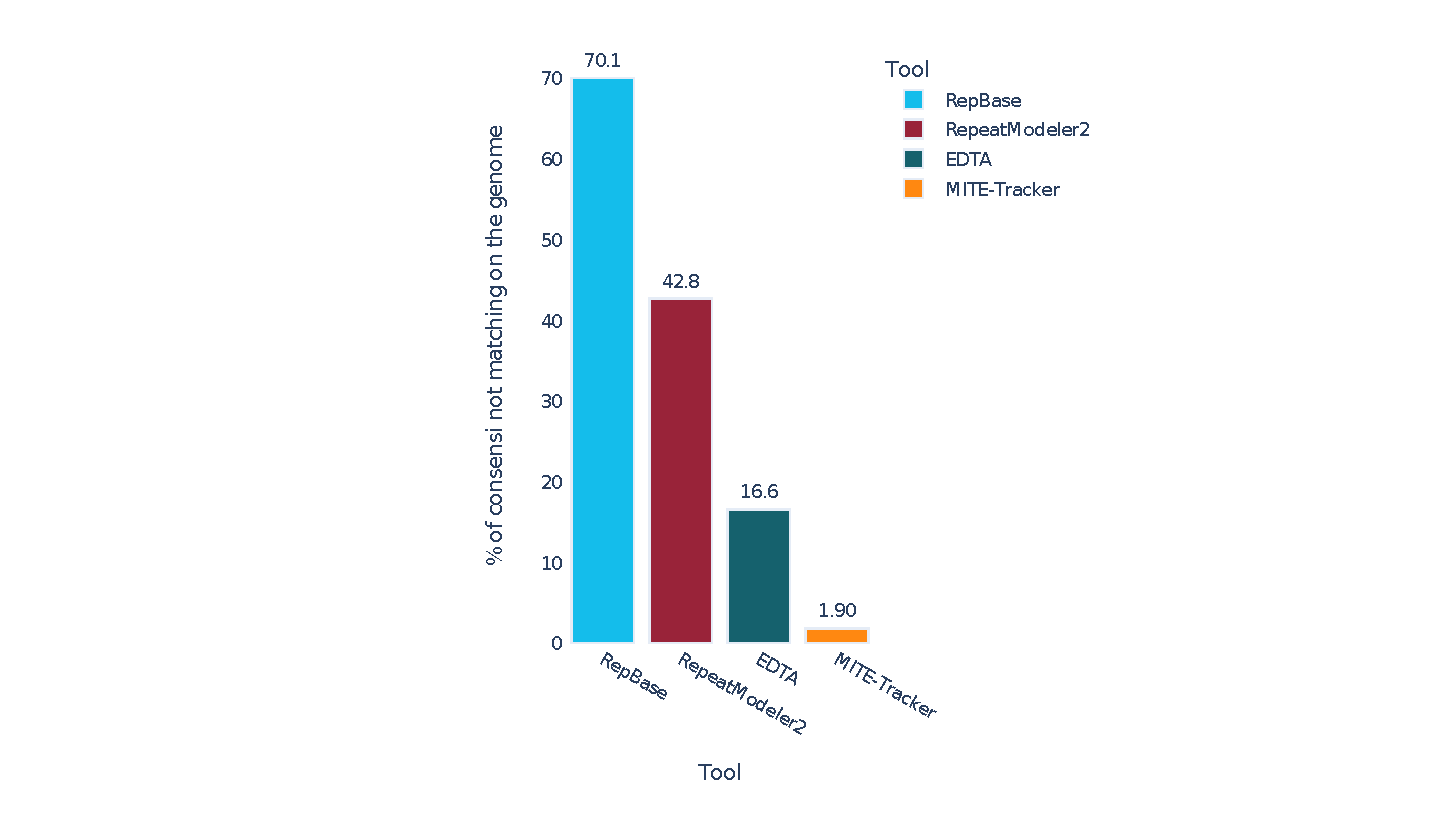
\includegraphics[width=\textwidth]{img/plots/nb_cons_by_tool.eps}
    \caption{Pourcentage des consensi qui n'ont pas eu de correspondance sur le génome pour chaque outil \textit{de novo} (plus \texttt{RepBase}).}
    %TODO resize and add caption description
    \label{fig:nb_cons_by_tool}
\end{figure}

\bigskip

En \figureautorefname{ \ref{fig:nb_cons_by_tool}} (\linkautorefname{\ref{link8}}), on peut observer le pourcentage de séquences pour chaque librairie de départ (\texttt{RepeatModeler2}, \texttt{EDTA}, \texttt{MITE-Tracker} et \texttt{RepBase}) qui n'ont pas masqué aucune portion du génome. \\
On observe que le 70.1\% des consensi contenus dans \texttt{RepBase} n'as pas de correspondance sur le génome. Cela est attendu en raison du fait que cette base de données contient des séquences provenant d'espèces différentes (séquences d'\textit{Arthropodes}), du coup même si il s'agit d'espèces phylogénétiquement proches à \textit{Ae. albopictus} il est possible qu'elles soient génétiquement distantes ou alors qu'elles possèdent un contenu en \acrlong{et} différent. \\
Parmi les outils \textit{de novo}, \texttt{RepeatModeler2} est celui en ayant le plus de séquences sans correspondance (42.8\%), suivi par \texttt{EDTA} (16.6\%) et \texttt{MITE-Tracker} (1.90\%). Le taux élévé de séquences qui ont pas été gardées pour \texttt{RepeatModeler2} est en partie explicable par la quantité de séquences redondantes (\tableautorefname{ \ref{tab:redondant_consensi}}), où 6 263 (40.71\%) séquences étaient des dupliqués. Du coup il reste plus que le 2.09\% de la librairie n'ayant réellement pas de correspondances sur le génome. De même pour \texttt{MITE-Tracker}, il y a que le 1.90\% des séquences qui ne sont pas retrouvées. \\
En revanche, \texttt{EDTA} montre un quantitatif important (16.6\%). Cela pourrait être expliqué par le fait que \texttt{RepeatMasker} mets en \og compétition \fg{} les fragments s'alignant sur une même portion de génome; dans ce cas, uniquement le hit avec le meilleur score sera conservé par le programme. Il est donc possible que \texttt{EDTA} ait détecté un certain nombre d'éléments déjà détectés par \texttt{RepeatModeler2} et, que ces derniers avaient un meilleur score d'alignement. Il est possible que le même mécanisme se soit mis en place avec les séquences dupliquées de \texttt{RepeatModeler2}, un meilleur hit (ou dans ce cas, équivalent) était déjà présent parmi les résultats et donc les séquences dupliqués n'ont pas été intégrées dans le fichier de sortie.  \\
Pour démontrer ce mécanisme de \texttt{RepeatMasker}, nous l'avons utilisé sur chaque librairies obtenues par les outils \textit{de novo} séparément, de façon à vérifier le nombre de consensi ayant des match pour chacune. En absence de compétition entre les différents librairies, on s'attend à voir une diminution des séquences n'ayant pas des correspondances sur le génome. Le résultat obtenu est montré dans le tableau suivant: \\

\bigskip

\begin{table}[H]
    \centering
    \begin{tabular}{r|c|c}
        \toprule 
        \textbf{Librairie} & \textbf{\makecell{Nb de séquences \\ n'ayant pas de match}} & \textbf{\makecell{\% sur la totalité \\ de la librairie}} \\
        \midrule
        \rowcolor{gray!10}
        \texttt{RepeatModeler2} & 6 440 & 41.86 \\
        \texttt{EDTA} & 298 & 1.84 \\
        \rowcolor{gray!10}
        \texttt{MITE-Tracker} & 76 & 0.70 \\
        \bottomrule
    \end{tabular}
    \caption{Nombre de séquences filtré par chaque librairie indépendamment en sortie de \texttt{RepeatMasker}.}
    \label{tab:nb_not_matching_tab}
\end{table}

\bigskip

Dans le \tableautorefname{ \ref{tab:nb_not_matching_tab}} on peut constater que \texttt{RepeatModeler2} a toujours un grand nombre de séquences n'ayant pas de match sur le génome (6 440), mais cela reste cohérent avec le nombre séquences dupliquées identifiées dans le \tableautorefname{ \ref{tab:redondant_consensi}}; ainsi si on les exclue, on obtient uniquement $6 440 - 6 263 = 177$ séquences n'ayant réellement pas de match (ce qui fait 1.15\% de la librairie brute de départ pour cet outil). Pour \texttt{EDTA} on peut voir que uniquement 298 séquences sont \og filtrées \fg{} par \texttt{RepeatMasker} et que donc le pourcentage de la librairie n'ayant pas de match passe de 16.6\% à 1.84\%. On constate une réduction aussi pour \texttt{MITE-Tracker} qui passe de 1.90\% à 0.70\%. \\
En conclusion, on montre que le fait d'utiliser \texttt{RepeatMasker} sur les différents librairies séparément ou sur une librairie finale a un impact sur le résultat final; utiliser directement une librairie fusionnée permet ainsi de réduire la redondance entre les différentes librairies de départ.


\subsubsection{Reconstruction des copies entières}

L'output de \texttt{RepeatMasker} a été ensuite filtré en fonction de la longueur des fragments. On a filtré tout fragment ayant moins de 80pb car on considère qu'ils ne sont pas assez longs pour apporter assez d'information dans les étapes suivantes. Le nombre de fragments passe donc de 8 966 074 à \textbf{6 596 866}. \\

Nous avons choisi ensuite d'utiliser \texttt{\acrshort{octfta}} pour reconstituer les solo-\acrshort{ltr} avec leur élément interne. Notamment il se base sur la recherche de séquences ayant le même préfixe dans le nom (ex. \textit{Gypsy}) mais avec des suffixes différentes: \textit{\acrshort{ltr}} pour les solo-\acrshort{ltr} et \textit{I} pour les éléments internes. \\
\'Etant donné qu'on a utilisé des outils différents et variés, il est possible que certains noms utilisés pour les séquences ne respectent pas ce format; pour cette raison nous avons choisi d'utiliser le paramètre \texttt{--insert} pour fusionner deux fragments se trouvant à moins de 80pb. \\

Après avoir exécuté \texttt{\acrshort{octfta}}, le nombre de séquences est passé à \textbf{4 304 741} instances. 

\bigskip

\subsubsection{Clustering des copies et appel des consensi}\label{sec:clustering_and_refining}


Les séquences ont été donc clusterisées en utilisant \texttt{cd-hit-est} pour pouvoir reconstituer les familles d'\acrlong{et} (règle 80-80-80). \\
Suite au clustering, on obtient \textbf{437 732} clusters:

\bigskip

\begin{table}[H]
    \centering
    \rowcolors{1}{gray!10}{}
    \begin{tabular}{c|c}
        \toprule
        Nb clusters larges (7 ou plus séquences) & 35 654 \\
        Nb clusters \og singleton \fg{} (une seule séquence) & 276 980 \\
        Nb clusters \og low copy \fg{} (entre 2 et 6 séquences) & 125 098  \\
        \midrule
        \textbf{Total} & \textbf{437 732} \\
        \bottomrule
    \end{tabular}
    \caption{Résultats de \texttt{cd-hit-est}.}
    \label{tab:results_cdhit}
\end{table}

\bigskip

Pour la suite de la construction de la librairie, on a choisi de ne garder que les clusters ayant un certain nombre de séquences (minimum 7) et on a choisi de séparer les restants en \og singleton \fg{}  (ayant une seule séquence) et en \og low copy \fg{} (entre 2 et 6 séquences). On a choisi de mettre de côté les \og singletons \fg{} car on estime que la majorité des \acrshort{et} est présent en plusieurs copies au sein du génome et, de façon similaire, les clusters \og low copy \fg{} ne sont également pas sélectionnés car on les attribue généralement à des \acrshort{et} qui sont peu actifs et, ils peuvent être facilement confondus avec d'autre éléments génomiques qui sont présentes en plusieurs copies (ex. des gènes paralogues \footnote{Gènes issus d'un événement de duplication.}). \\
Le nombre minimal de séquences au sein d'un cluster est donc directement lié à la répétitivité minimale attendue pour n'importe quelle famille; en \figureautorefname{ \ref{fig:nb_clst}} (\linkautorefname{\ref{link10}}) on peut voir comme le nombre de clusters peut varier sensiblement en fonction du nombre minimal de séquences formant les clusters. \\

\bigskip

\begin{figure}[H]
    \centering
    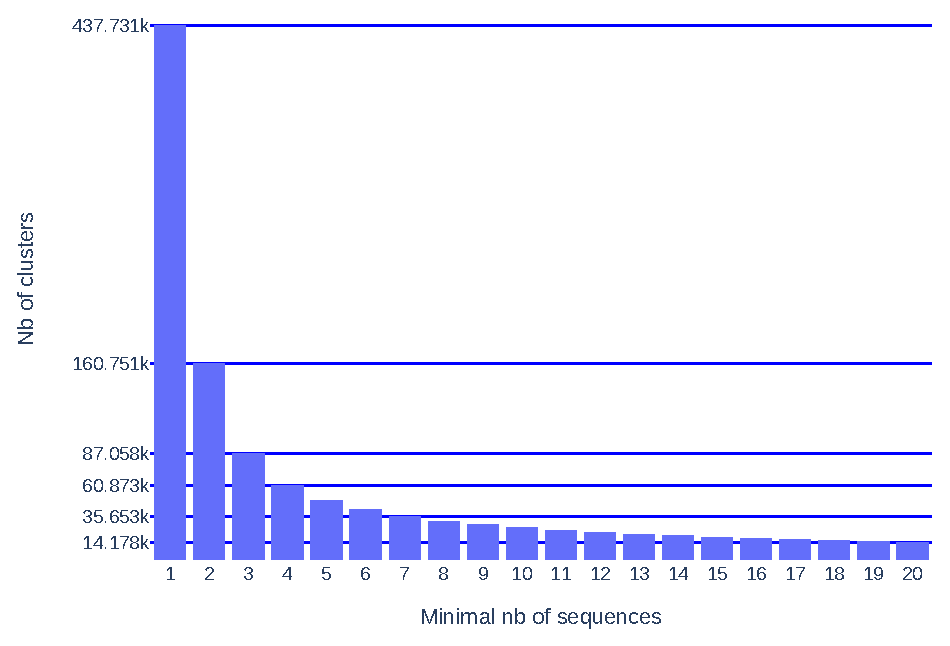
\includegraphics[width=\textwidth]{img/plots/nb_clust_by_min.eps}
    \caption{Nombre de clusters en fonction du nombre minimal de séquences formant le cluster.}
    \label{fig:nb_clst}
\end{figure}

\bigskip

On peut voir comme en sélectionnant au minimum deux séquences on réduit considérablement le nombre de clusters (de 437 761 à 160 751 clusters). En prenant 7 séquences ou plus (comme on l'a fait dans notre démarche), on obtient que 35 653 clusters et, si on passe à 20 séquences on réduit le nombre à 14 178 clusters. \\
On aurait pu, sans doute utiliser 20 séquences comme seuil minimal pour réduire le temps de calcul dans les étapes qui ont suivi, mais on aurait risqué de perdre certaines des familles les moins actives, étant elles présentes en un nombre limité de copies.  \\

Ensuite, on s'est également interrogés sur la contribution de chaque librairie de départ dans la formation des clusters (clusters respectant le seuil de séquences minimales, au premier cycle), \figureautorefname{ \ref{fig:contribution}}. Parmi les 35 654, il y en a 191 qui sont formés uniquement par des séquences provenant de \texttt{RepBase}, 5 740 de \texttt{RepeatModeler2}, 3 821 d'\texttt{EDTA} et 423 de \texttt{MITE-Tracker}. \\
En détail, \texttt{RepBase} participe dans un total de 3 407 clusters, soit un peu moins d'un dixième (9.55\%) du total et, permet d'avoir un ensemble fiable d'\acrshort{et}; \texttt{RepeatModeler2} dans 29 206 (soit 81.92\%); \texttt{EDTA} dans 28 015 (soit 78.57\%) et; \texttt{MITE-Tracker} dans 11 066 (soit 31.04\%). \\
On note que l'intersection entre \texttt{RepeatModeler2} et \texttt{EDTA} est de 12 768 clusters et celle entre ces deux plus \texttt{MITE-Tracker} est de 6 959. Ces chiffres permettent de souligner l'intérêt d'une stratégie utilisant une annotation \textit{de novo}. \\
Les séquences provenant de \texttt{MITE-Tracker} et qui sont retrouvées dans des clusters avec des séquences provenant d'autres outils (1 056 + 6 959) pourrait laisser penser que \texttt{MITE-Tracker} a classifié par erreur certains éléments, autres que des \acrshort{mite}, comme des \acrshort{mite}. Cela paraît évident si on pense un nombre de \acrshort{mite} contenus dans \texttt{RepBase} (10 séquences). Cependant, il faut garder en tête que, il s'agit d'un type d'\acrshort{et} qui a été décrit plus récemment que d'autres et que donc pour cela, sa représentation dans les bases de données est logiquement moindre. \\
De même, le nombre de clusters outil-spécifique \texttt{RepeatModeler2} et \texttt{EDTA} pourrait suggérer la présence de faux positifs, mais cela reste compliqué à déterminer, surtout que les deux utilisent des approches différentes dans la détection.

\bigskip

\begin{figure}[h]
    \centering
    %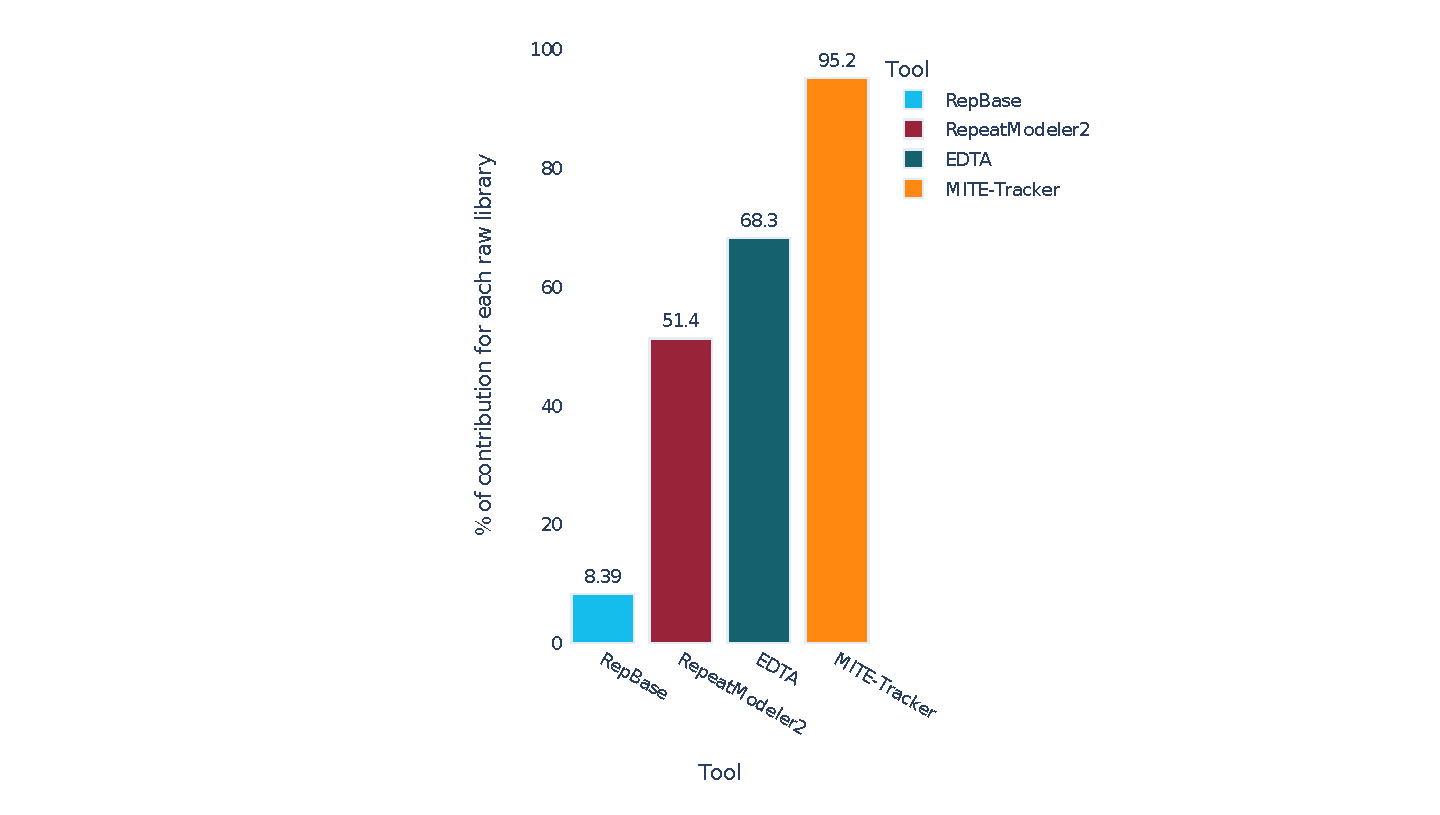
\includegraphics[width=\textwidth]{img/plots/contribution.eps}
    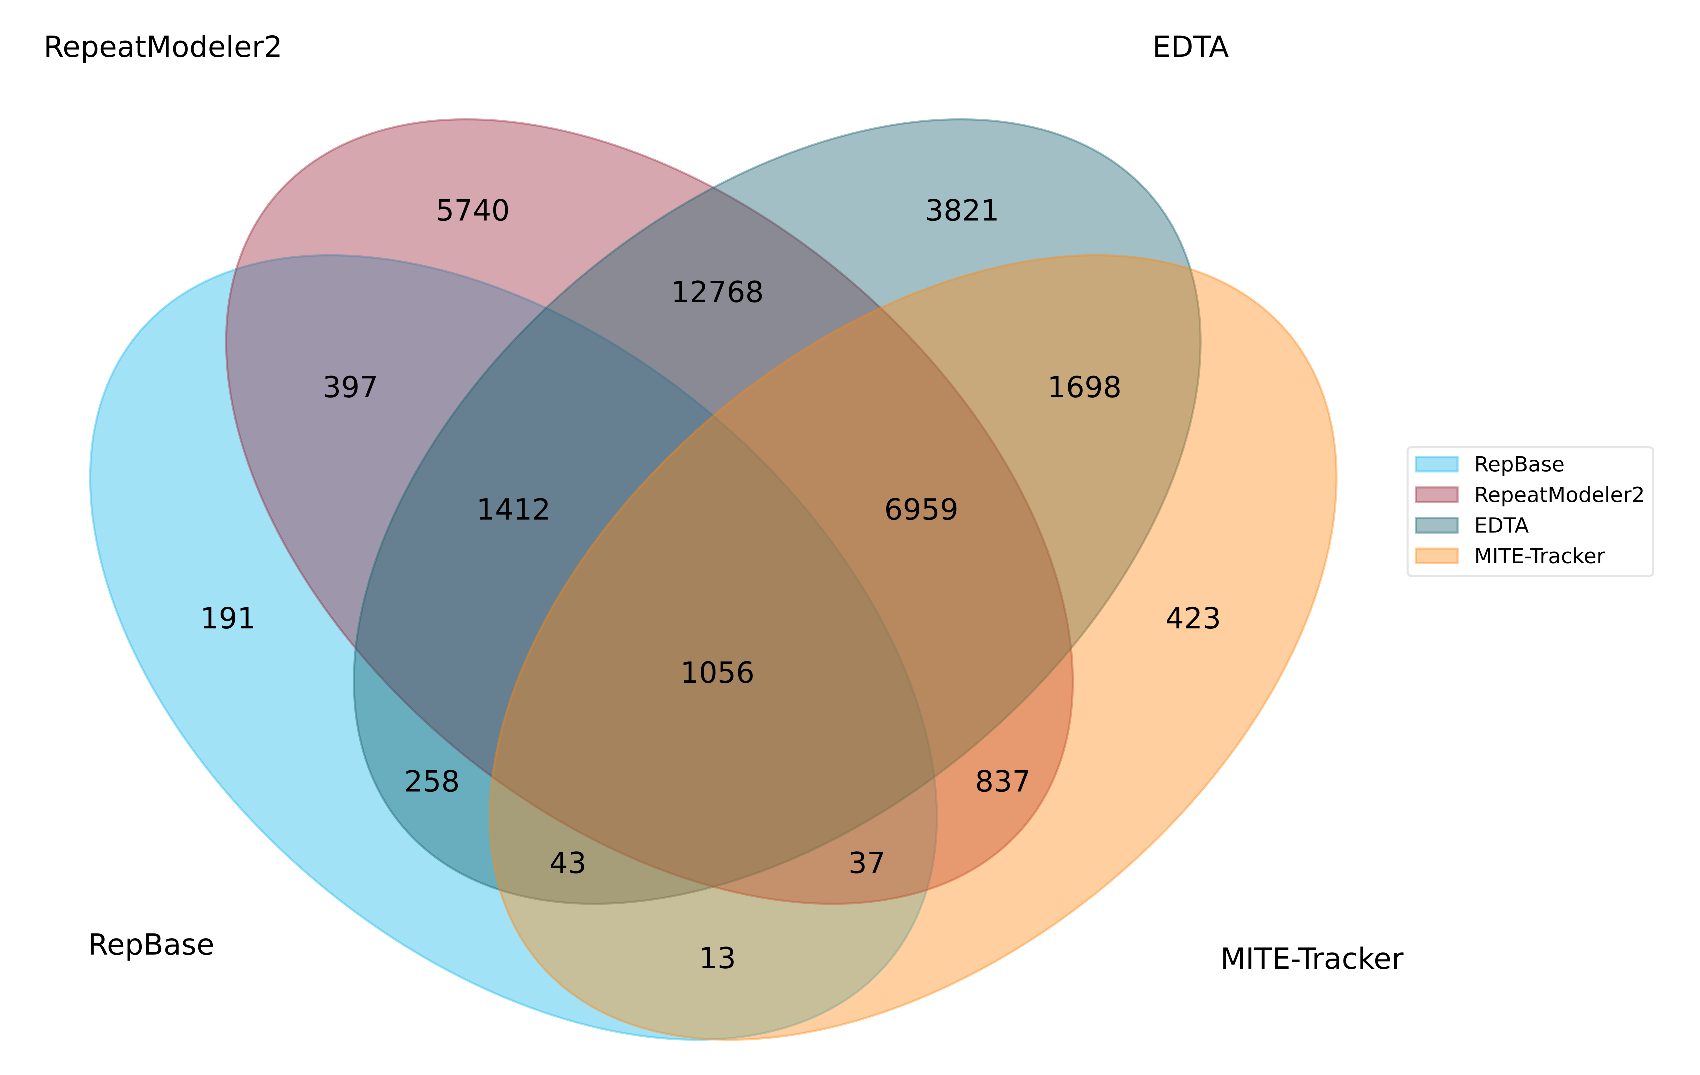
\includegraphics[width=\textwidth]{img/plots/contribution_venn.eps}
    \caption{Contribution de chaque librairie de départ dans la formation des clusters.}
    \label{fig:contribution}
\end{figure}

\bigskip

%Sur l'axe des ordonnées, on peut donc trouver le pourcentage de séquences de la librairie de départ ayant contribué dans au moins un cluster. \\ 
%On peut observer que, comme attendu \texttt{RepBase} est la librairie qui a contribué le moins (8.39\%) tandis que  \texttt{MITE-Tracker} est elle qui a contribué le plus (95.2\%). \texttt{EDTA} a eu 68.3\% des séquences contribuant alors que pour \texttt{RepeatModeler2} c'est que le 51.4\%. \\


Pour chacun des clusters conservés, on a appelé un consensus en utilisant \texttt{Refiner}. Comme indiqué dans \subsectionautorefname{ \ref{subsec:lib_construction}}, pour cette étape on n'a pas utilisé le nombre total de séquences de chaque cluster. Le nombre de séquences conséquent  de certains cluster était beaucoup trop élévé pour permettre l'exécution de \texttt{Refiner} dans un délai de temps raisonnable. On a choisi d'échantillonner un maximum de 500 séquences car c'est suffisant pour réduire le temps de calcul et puis car une analyse préliminaire a permis de montrer que ce nombre de séquences est suffisant pour avoir un consensus stable. 
% Dans cette analyse on a échantillonné au hasard 40 clusters ayant 500 séquences ou plus. Pour chacun, on a effectué un échantillonnage aléatoire de: 100, 150, 200, 250, 300, 350, 400, 450 et 500 séquences. Sur chaque échantillonnage de chaque cluster, on a ensuite exécuté \texttt{Refiner} pour obtenir une séquence consensus. \\
% Le résultat obtenu est montré en \figureautorefname{ \ref{fig:sampled_cluster}}; on peut observer l'allure de la longueur du consensus pour chaque cluster en fonction des différents échantillonnages. \\
% On peut observer que, à exception de deux clusters (16 et 39), les clusters ont globalement une allure linéaire par rapport à la longueur du consensus. On conclu ainsi que, 500 séquences permettent d'apporter assez d'information pour avoir un consensus fini, le tout en réduisant de manière important le temps de calcul.

% \bigskip

% \begin{figure}[H]
%     \centering
%     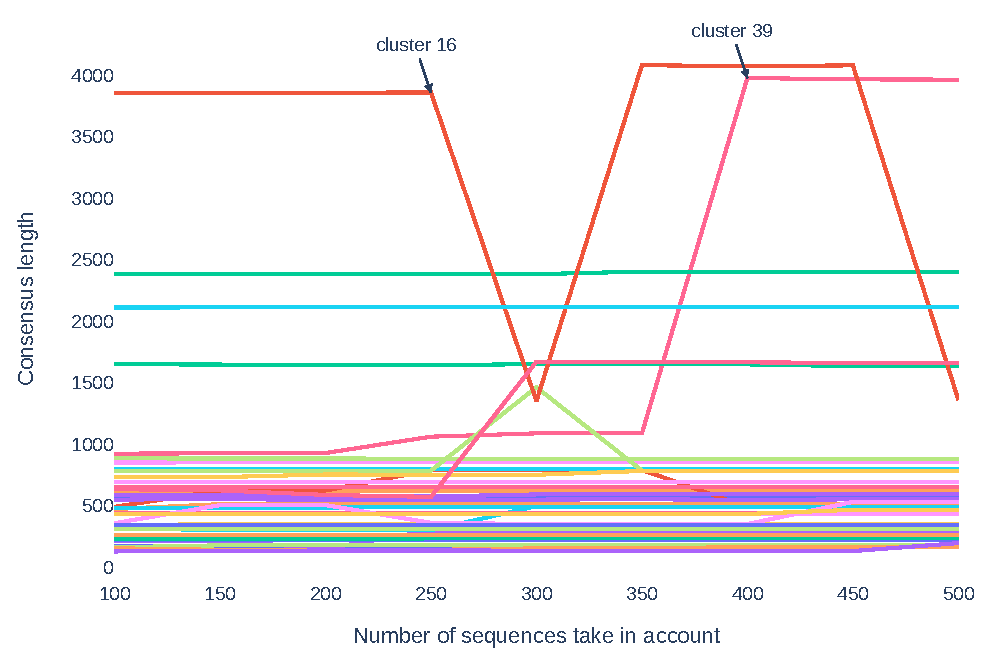
\includegraphics[width=0.9\textwidth]{img/plots/cluster_sample.eps}
%     \caption{Longueur du consensus en fonction du nombre de séquences échantillonnées au sein du cluster.}
%     \label{fig:sampled_cluster}
% \end{figure}

% \bigskip

Enfin, on a réalisé plusieurs cycles (7) \texttt{cd-hit-est}/\texttt{Refiner} de façon à réduire un maximum la redondance. \`A différence du premier cycle, à chaque itération on a conservé tous les clusters et on a pas eu besoin de re-effectuer un sous-échantillonnage des séquences intra-cluster. On obtient ainsi un total de  \textbf{23 009} séquences. \\

 %\texttt{dnaPipeTE} a permis de montrer que ces consensi masquent 67\% du génome de référence. On couvre ainsi 10\% en moins que prédit par \texttt{RepeatModeler2} et \texttt{EDTA} (\tableautorefname{ \ref{tab:results_annotation}}) mais beaucoup plus que les librairies produites par d'autres auteurs (\autoref{tab:annot_state_of_art}).

\bigskip

\subsection{Polissage des extrémités} Pour améliorer la qualité des consensi on a choisi d'effectuer un polissage des extrémités. Cela peut consister en deux types d'action, l'extension ou la troncature. \`A cet effet nous avons écrit un pipeline décrit dans le \paragraphautorefname{ \ref{sec:polish}}. \\
%Cette étape peut se révéler importante, voire indispensable, pour le génotypage et l'identification de nouvelles insertions sur des nouveaux génomes, en particulier avec des programme utilisant un approche \acrfull{sr} (voir \subsectionautorefname{ \ref{sec:geno}} \textsc{Génotypage}). 


\paragraph{\'Evaluation du pipeline} Pour tester l'efficacité du programme, nous avons créé un petit jeu de données ne contenant que des \acrlong{et} connus et annotés dans \texttt{RepBase25.08} de l'espèce \textit{Drosophila melanogaster}, car étant une espèce modèle, ses \acrlong{et} sont parmi ceux les mieux annotés. On a ainsi artificiellement tronqué les extrémités de ces séquences (\linkautorefname{\ref{link11}}), 10\% de la longueur originale pour chaque extrémité, et on a utilisé le programme en utilisant l'assemblage \texttt{ASM2016949v1} (obtenu par technologie de séquençage \acrlong{lr} - \texttt{Nanopore MinION}). \\
Le jeu de données utilisé contient au total 180 séquences. 179 ont été polies tandis qu'une seule séquence a été détectée comme des \acrshort{ssr}. Parmi les 179 séquences traitées, \textbf{155} ont été étendues et \textbf{24} ont été tronquées ultérieurement. L'extension minimale (par rapport à la séquence tronquée artificiellement) a été de 0\% et celle maximale de 314\% , avec une médiane de 40\%; la troncature minimale a été de 1\% et celle maximale de 50\%, avec une médiane de 12\%. \\

\bigskip

\begin{figure}[h]
    \centering
    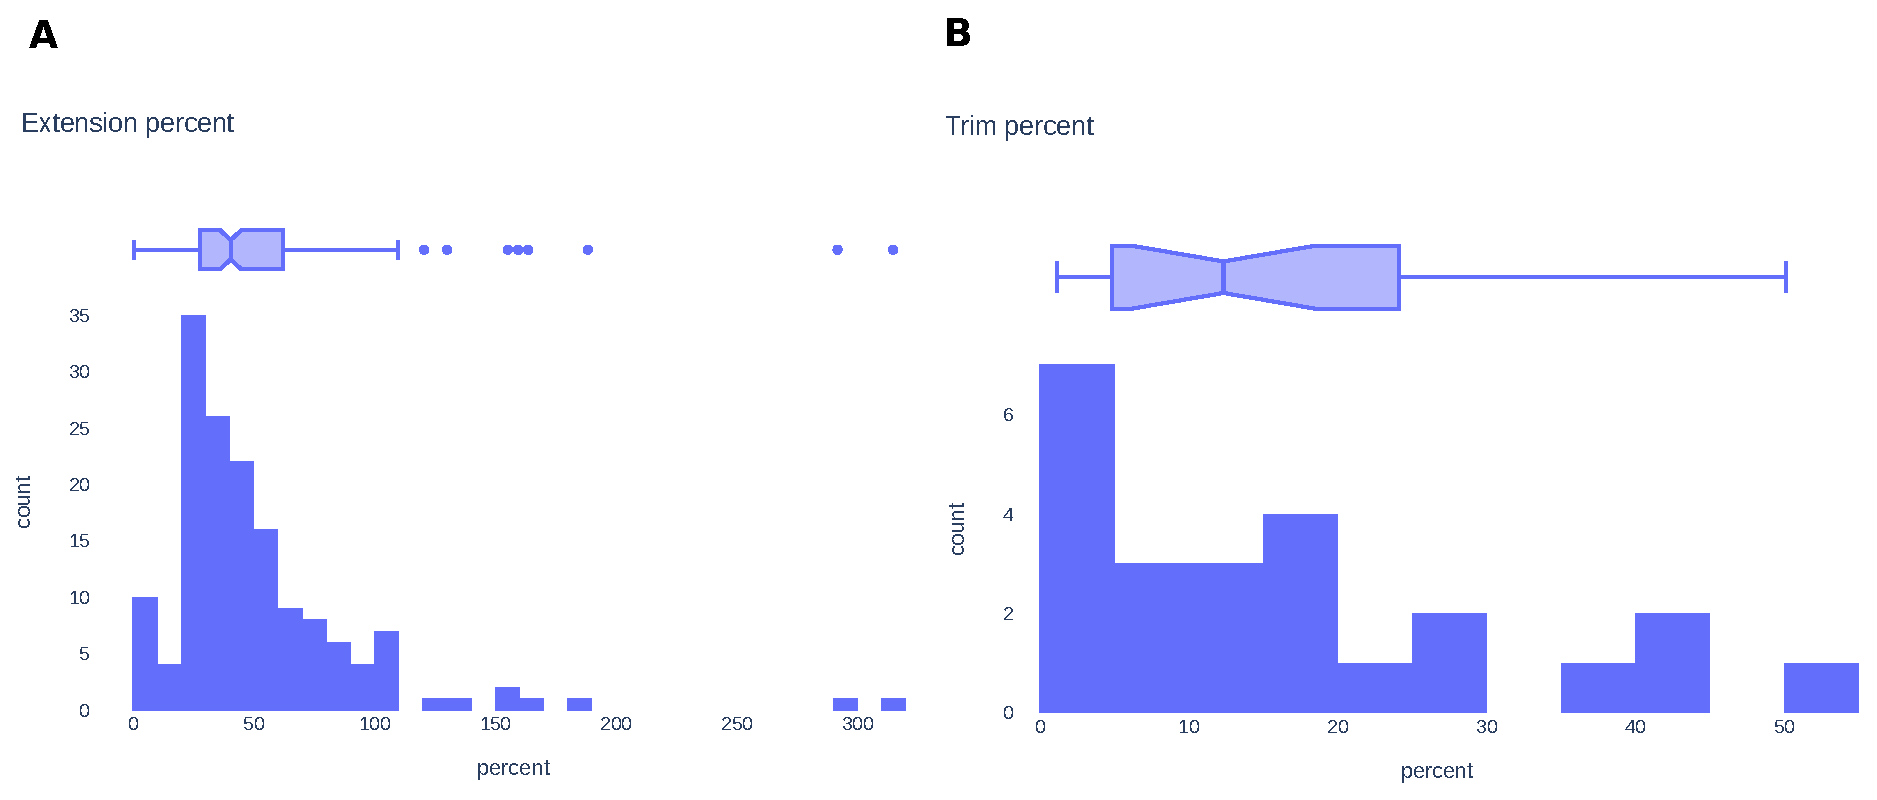
\includegraphics[width=\textwidth]{img/plots/droso_polish.eps}
    \caption{Pourcentage d'extension et de troncature sur le jeu de données de test.}
    \caption*{
    \scriptsize{
    \textbf{A} - Distribution des pourcentages d'extension; \textbf{B} - Distribution des pourcentages de troncature.
    }
    }
    \label{fig:droso_polish_stats}
\end{figure}


L'attendu était de n'avoir que des séquences étendues et, spécialement avec une extension moyenne de 25\% (pour retrouver les extrémités tronquées artificiellement). Or, ce n'est pas le cas de nos résultats, donc on a choisi d'inspecter un peu plus les séquences tronquées de départ et les séquences traitées avec le pipeline et, d'évaluer certains critères, comme le nombre de fragments obtenus en réalisant un \texttt{blastn} sur le génome de référence (plus le nombre est élevée, plus la famille est mieux représentée), le nombre de copies entières (étant une copie entière un fragment ayant au moins 90\% de la longueur du consensus), la conservation (ou amélioration) de la détection des domaines protéiques, la divergence\footnote{
La divergence d'une copie du consensus traduit d'une certaine manière la distance entre les deux séquences. Lors de l'évolution, des copies différentes d'un même élément peuvent accumuler de façon différente des mutations, engendrant une divergence propre à chaque copie. \\
\'Etant la séquence consensus d'une famille, la séquence \og moyenne \fg{} représentant l'ensemble des copies de cette famille, il est important de minimiser sa distance (ou donc en autre termes, la divergence) avec les membres de la famille.
} 
des copies entières (moins elles sont divergentes, plus ça signifie que le consensus les représente de manière correcte) et, enfin la couverture génomique des extrémités. Pour évaluer tous ces critères, on a utilisé un outil pour la vérification manuelle des \acrshort{et}, \texttt{TE-Aid} \cite{goubert_beginners_2022}. \\

Dans le \tableautorefname{ \ref{tab:eval_poliste}}, on peut observer les résultats de cette évaluation. On peut noter que le nombre moyen de fragments a augmenté sensiblement de 94.8 à 164.8, ce qui est plutôt bien en considérant le fait que plus de fragments sont trouvés sur le génome correspondant à la séquence consensus, mieux elle représente l'ensemble des copies. \\
Le nombre moyen de copies entières a aussi augmenté, mais cette fois-ci la différence est moins éclatante; bien que il soit important, quand possible, de récupérer la totalité des copies entières, il faut préciser que dans des nombreux cas l'augmentation a été observée sur des séquences qui ont été tronquées; or en réduisant la taille de la séquence il va de soi qu'il soit plus facile d'obtenir des copies entières. \\
Pour 158 séquences sur 179 on a pu retrouver (ou même améliorer) les domaines protéiques annotés par \texttt{TE-Aid}. On a pu remarquer que les consensi n'ayant pas conservé leur domaines protéiques c'était des séquences qui ont eu une forte augmentation du nombre de fragments après polissage et que ceux-ci, en particulier se chevauchent à certains endroits sur le consensus, suggérant que certaines nucléotides (en correspondance des chevauchements) sont incorrects. \\
Concernant la divergence des copies entières par rapport à la séquence consensus, on a constaté une diminution dans 48 cas, aucune différence pour 67 séquences et, une augmentation dans 63 cas. D'une part, la diminution de la divergence se traduit avec une meilleure description de la famille d'\acrshort{et} mais d'autre part, l'augmentation de la divergence couplée à l'augmentation du nombre de copies entières peut aussi être synonyme d'une meilleure représentation car, les membres les plus anciens d'une famille sont connus pour avoir une forte divergence par rapport à les copies les plus récentes. \\
Enfin, nous avons pu constater une amélioration de la couverture sur l'extrémité 5' dans 95 cas sur 179 et dans 90 cas sur 179 pour l'extrémité 3'. \\

\bigskip

\begin{table}[h]
    \centering
    \begin{tabular}{r|c|c}
        \toprule 
         & \textbf{Avant polissage} & \textbf{Après polissage} \\
        \midrule
        Nombre moyen de fragments & 93.8 & 163.8 \\
        \rowcolor{gray!10}
        Nombre moyen de copies entières & 17.9 & 18.5 \\
        \makecell{Conservation/Amélioration \\ des domaines protéiques} & \multicolumn{2}{c}{158 sur 179} \\
        \rowcolor{gray!10}
        Divergence des copies entières & \multicolumn{2}{c}{48 -, 67 =, 63 +} \\
        Amélioration couverture en 5' & \multicolumn{2}{c}{95 sur 179} \\
        \rowcolor{gray!10}
        Amélioration couverture en 3' & \multicolumn{2}{c}{90 sur 179} \\
        \bottomrule
    \end{tabular}
    \caption{\'Evaluation du pipeline pour le polissage.}
    \caption*{
    \scriptsize{
    Divergence des copies entières: \textbf{"-"} indique que le nombre de copies entières après polissage ayant moins de divergence qu'avant; \textbf{"="} indique pas de changement; \textbf{"+"} indique une augmentation de la divergence.
    }
    }
    \label{tab:eval_poliste}
\end{table}

\bigskip

Pour clarifier ce qu'on entend par amélioration de la couverture, un exemple bien réussi est montré en \figureautorefname{ \ref{fig:BURDOCK}}. Dans un premier temps on peut noter la longueur du consensus avant et après polissage, on passe de 4 688pb à 6 426pb, ce qui fait une extension de 37\%, donc c'est plus que l'attendu moyen (25\%) mais ça reste tolérable. \\
Ensuite on peut voir que le nombre de fragments a presque doublé, de 68 à 119 fragments et que le nombre de copies à longueur entière (en rouge, sur le graphique de divergence des hits \texttt{blastn}, en haute à gauche) n'a pas bougé (5 copies). \\
Sur le graphique de la couverture génomique, on retrouve le même profil à une exception près: on peut noter comme la couverture sur les deux extrémités soit augmenté de façon considérable après polissage et, comme l'extension se soit arrêtée juste après ces deux pics. Ce qui c'est passé c'est la chose suivante: la séquence avant traitement présentait uniquement l'élément interne d'un \acrshort{ltr} (comme démontré par l'annotation des domaines protéiques) et, le pipeline dans la séquence traitée a permis de récupérer les \acrfull{ltr} proprement dit présents aux extrémités. \\ 
Cela se confirme à la fois sur le \textit{self dotplot} (en bas à gauche), lequel montre des répétions directes aux extrémités (les traits parallèles à la diagonale), et à la fois sur l'annotation des structures et des domaines protéiques avec les flèches vertes dans le même sens. \\
Enfin, mais pas moins important, on retrouve l'annotation des domaines protéiques avant et après polissage (\textit{Gag} + \textit{Pol}). \\

\bigskip

\begin{figure}[h]
    \centering
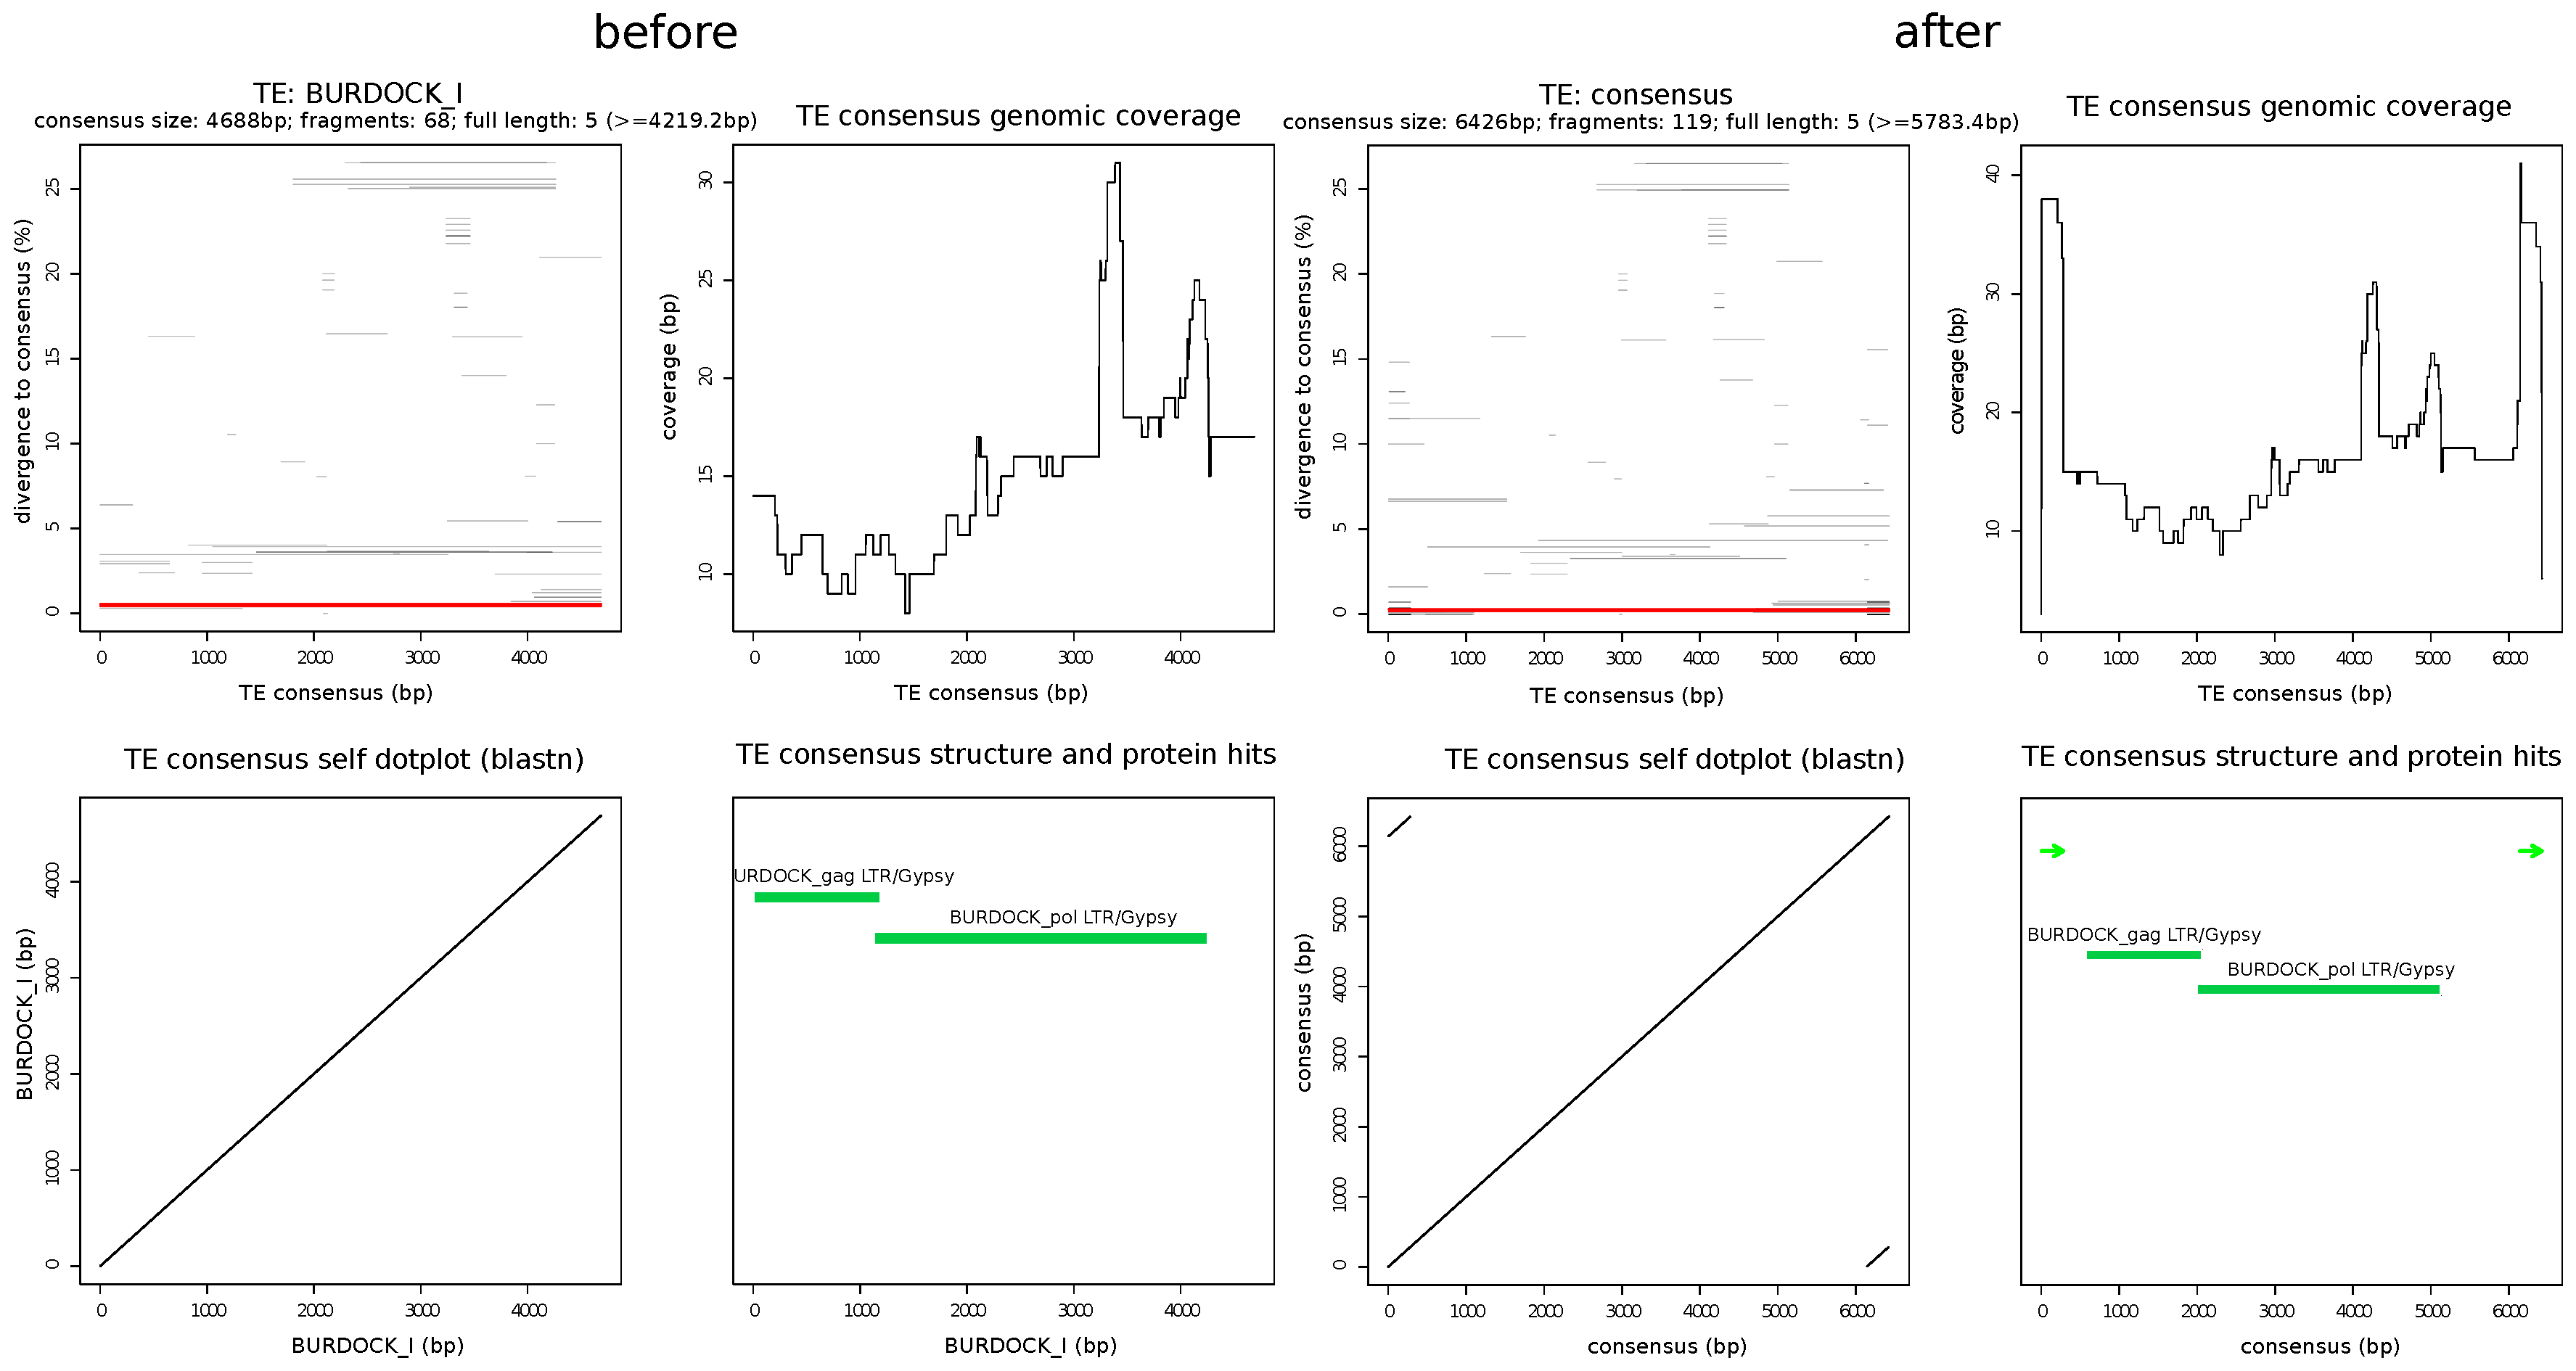
\includegraphics[width=\textwidth]{img/plots/burdock.eps}
    \caption{Résultats de \texttt{TE-Aid} pour l'élément \textbf{BURDOCK\_I}.}
    \caption*{\scriptsize
    \textit{En haute à gauche}: divergence et position par rapport au consensus des hits (\texttt{blastn}), en rouge les hits considérés comme des copies à longueur entière; \textit{en haute à droite}: couverture génomique du consensus par les hits; \textit{En bas à gauche}: le \textit{self dotplot} de la séquence (\texttt{blastn} de la séquence consensus contre elle-même); \textit{En bas à droite}: annotation des structures caractéristiques des \acrshort{et} et hits contre une bases de données de domaines protéiques (\texttt{RepeatPeps} (\texttt{RepeatMasker})). \\
    \textbf{Before} - Résultats de pour l'élément BURDOCK\_I tronqué artificiellement. \textbf{After} - Résultats après polissage.
    }
    \label{fig:BURDOCK}
\end{figure}

\bigskip

Pour retourner à l'évaluation du pipeline, il est important de signaler les choses suivantes: la plupart des meilleurs exemples étaient des éléments internes de \acrshort{ltr} (comme en \figureautorefname{ \ref{fig:BURDOCK}}); lors du traitement de certains solo-\acrshort{ltr}, le programme a essayé d'aller chercher l'élément interne correspondant mais cela à généralement aboutit dans nombreux fragments se chevauchant de manière irrégulière (en raison du fait que l'élément interne peut être récupéré à la fois en allant vers la gauche à partir du solo-\acrshort{ltr} en 3' et à la fois en allant vers la droite à partir du solo-\acrshort{ltr} en 5'); les séquences ayant subi une forte troncature (au délà du 30\%) étaient toutes des familles \textit{TART} ou \textit{TARHE} (non-\acrshort{ltr}); enfin, qu'une majorité des séquences testées étaient des \acrshort{ltr}. \\ 

\bigskip

\paragraph{Résultats polissage} Le pipeline a été donc utilisé pour polir les séquences contenues dans la notre librairie. Les distributions des pourcentages d'extension et de troncature sont montrées en \figureautorefname{ \ref{fig:polishte_put_data}}. \\
Sur 23 009 séquences, 19 939 ont été polies et des 3 070 restantes, 610 sont des \acrshort{ssr} et 2 460 n'ont pas été modifiées. Parmi les séquences polies, 14 364 ont été étendues et 5 575 ont été tronquées. \\
L'extension minimale est de 0\%, la maximale de 465\% et la médiane est à 28\%; la troncature minimale est de 0\%, la maximale de 93\% et la médiane à 13\%. \\
Pour vérifier le bon fonctionnement du pipeline, tout comme pour le test, nous avons utilisé \texttt{TE-Aid} sur 10 séquences. Quelques exemple sont montrés en \textsc{\ref{s:annexes}} (\autoref{fig:seq_4} à \autoref{fig:seq_19422}). Sur ceux-ci on peut constater une amélioration globale des séquences avec des extrémités bien polies (ex. \autoref{fig:seq_4}), une forte augmentation de fragments (ex. \autoref{fig:seq_4547}) ou encore une nouvelle récupération de \acrshort{ltr} (ex. \autoref{fig:seq_19422}). \\

\begin{figure}[H]
    \centering
    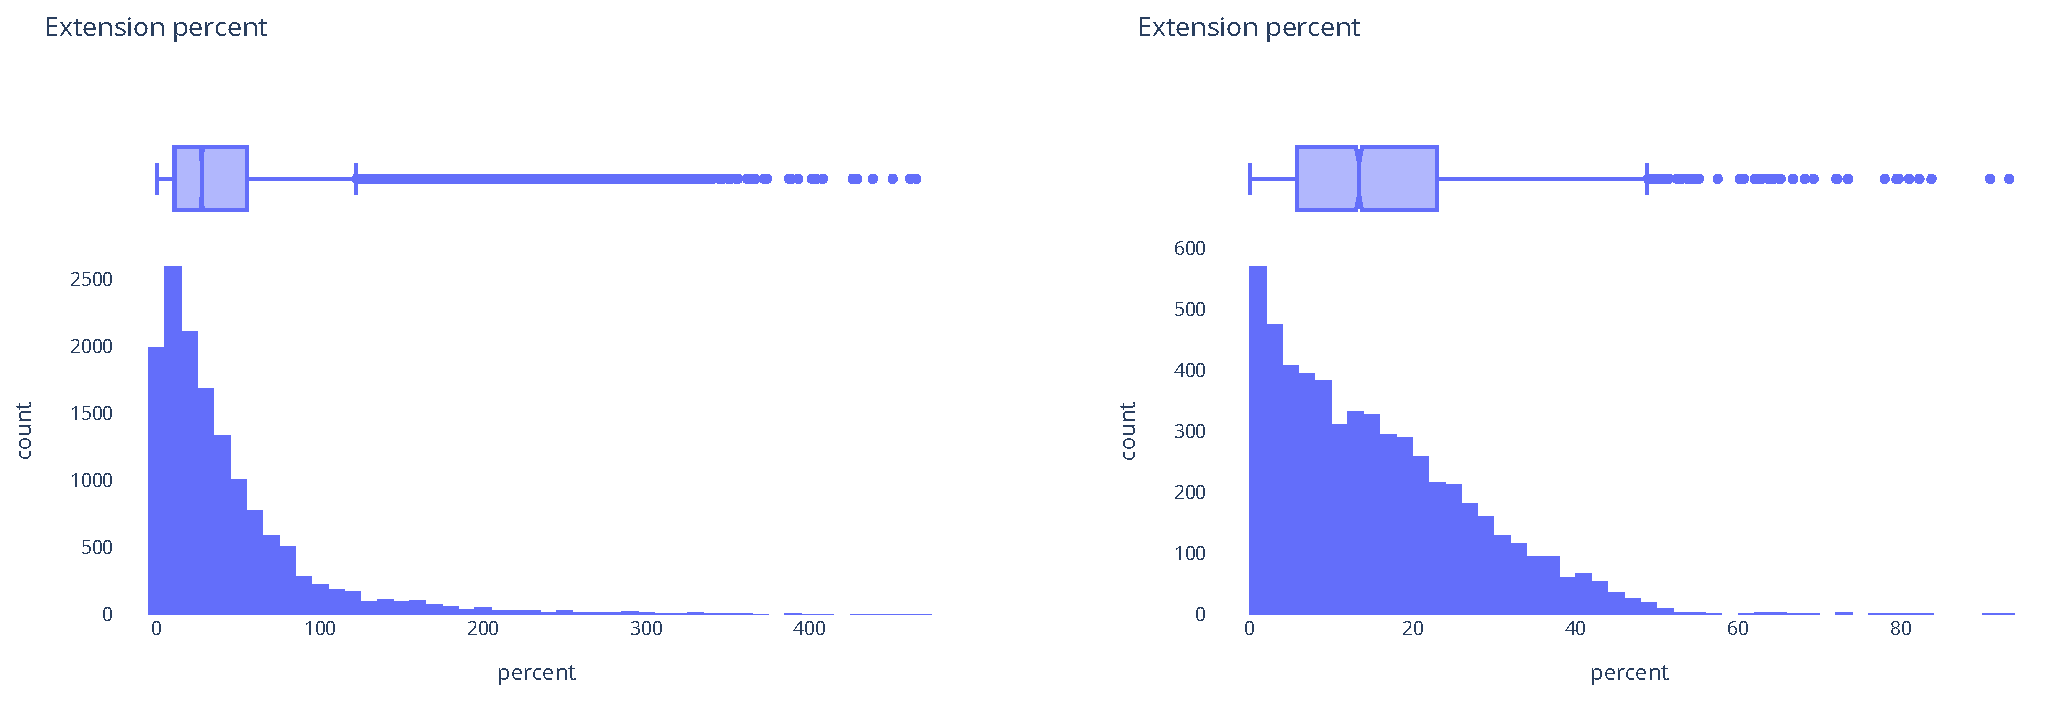
\includegraphics[width=\textwidth]{img/plots/polish_putative_data.eps}
    \caption{Distributions des pourcentage d'extension et de troncature sur nos données.}
    \label{fig:polishte_put_data}
\end{figure}

\bigskip
% \newpage

\subsection{Classification}

La classification a été réalisé sur les \textbf{23 009} séquences traitées avec le pipeline pour le polissage. On a gardé donc les séquences marquées comme \acrshort{ssr} dans le but de les conserver pour ensuite avoir une idée globale sur le contenu d'éléments répétés (du coup \acrlong{et} ou pas) dans le génome d'\textit{Ae. albopictus}.

\bigskip

\paragraph{Résultats des outils de classification} \textit{ } \\

\bigskip

\begin{itemize}
    \item[\ding{42}] \texttt{RepeatMasker}: en sortie on obtient un total de 86 695 hits sur des consensi contenus dans \texttt{RepBase27}. Après avoir filtré en fonction de la divergence et la longueur de l'alignement sur la séquence analysée, on obtient 17 671 hits (dont 8 065 séquences uniques sur les 23 009 séquences traitées). \\
    \begin{table}[H]
        \centering
        \begin{tabular}{r|c}
            \toprule
            \textbf{Classification} & \textbf{Effectif} \\
            \midrule
            \rowcolor{gray!10}
            DNA & 2 257 \\
            \acrshort{line} & 1 135 \\
            \rowcolor{gray!10}
            \acrshort{ltr} & 3 471 \\
            \acrshort{mite} & 37 \\
            \rowcolor{gray!10}
            non-\acrshort{ltr} & 418 \\
            \acrshort{sine} &  394 \\
            \rowcolor{gray!10}
            Unknown & 72 \\
            \bottomrule
        \end{tabular}
        \caption{Classification selon \texttt{RepeatMasker} en utilisant \texttt{RepBase}}
        \label{tab:repdfam_results}
    \end{table}
    \item[\ding{42}] \texttt{RepeatProteinMask}: on obtient un total de 160 643 hits sur les séquences de \texttt{RepeatPeps.lib}. Après filtrage sur le score d'alignement (>200) et sur la longueur de l'alignement sur la séquence analysée (query), on obtient 4 626 séquences uniques sur les 23 009 séquences traitées. \\
    
    \begin{table}[H]
        \centering
        \begin{tabular}{r|c}
            \toprule
            \textbf{Classification} & \textbf{Effectif} \\
            \midrule
            \rowcolor{gray!10}
            DNA & 98 \\
            \acrshort{line} & 1 909 \\
            \rowcolor{gray!10}
            \acrshort{ltr} & 2 501 \\
            \acrshort{rc} & 6 \\
            \rowcolor{gray!10}
            \acrshort{ssr} & 111 \\
            \bottomrule
        \end{tabular}
        \caption{Classification selon \texttt{RepeatProteinMask}}
        \label{tab:repcprotmask_results}
    \end{table}
    
    \item[\ding{42}] \texttt{RepeatClassifier}: cet outil attribue directement une classification (quand possible) à la séquence traitée, pour cette raison aucune étape de filtrage est nécessaire ici. Les effectifs pour chaque groupe d'\acrshort{et} sont montrés dans le tableau suivant: \\
    \begin{table}[H]
        \centering
        \begin{tabular}{r|c}
            \toprule
            \textbf{Classification} & \textbf{Effectif} \\
            \midrule
            \rowcolor{gray!10}
            DNA & 951 \\
            \acrshort{line} & 2 335 \\
            \rowcolor{gray!10}
            \acrshort{ltr} & 3 092 \\
            \acrshort{rc} & 1 101 \\
            \rowcolor{gray!10}
            \acrshort{sine} & 142 \\
            tRNA & 190 \\
            \rowcolor{gray!10}
            Unknown & 15 223 \\
            \bottomrule
        \end{tabular}
        \caption{Classification selon \texttt{RepeatClassifier}}
        \label{tab:repclassifier_results}
    \end{table}

\end{itemize}

\bigskip

\paragraph{Fusionnement des résultats} Comme expliqué en \sectionautorefname{ \ref{sec:classif_sec}}, on a attribué à une séquence une classification si et seulement si au moins deux outils ont eu le même résultat (d'abord au niveau de la super-famille et puis, où possible, au niveau de la famille). Les effectifs des super-familles identifiées sont montrés dans le tableau suivant: \\

\bigskip

\begin{table}[H]
    \centering
    \begin{tabular}{r|c}
        \toprule
        \textbf{Classification} & \textbf{Effectif} \\
        \midrule
        DNA & 624  \\
        \rowcolor{gray!10}
        \acrshort{ltr} & 2 742 \\
        \acrshort{line} & 1 983 \\
        \rowcolor{gray!10}
        %rRNA & 2 \\
        \acrshort{ple} & 9 \\
        %\rowcolor{gray!10}
        \acrshort{sine} & 45 \\
        \rowcolor{gray!10}
        \acrshort{ssr} & 39 \\
        %snRNA & 1 \\
        \midrule
        \rowcolor{gray!10}
        \textbf{Total} & 5 442 \\
        \bottomrule
    \end{tabular}
    \caption{Résultat combiné des différents outils de classification.}
    \caption*{
    \scriptsize{
    Dans ce tableau, on a délibérément omis les éléments suivants: rRNA (2 séquences), Satellites (19), snRNA (1) et tRNA(1).
    }
    }
    \label{tab:merged_classif}
\end{table}

\bigskip

%Après \texttt{einverted}, 711 \acrshort{mite} et 1 103 \acrshort{tir} sont rajoutés à les séquences précédemment classifiées. 
Les premières 20 séquences les plus répétées ainsi que les 20 ayant le plus de couverture génomique on été vérifiées manuellement (\linkautorefname{\ref{link12}}) et lorsqu'il a été possible de renseigner au moins la super-famille, la séquence a été rajoutée, en atteignant un total de 5 465 séquences classifiées. \\
En \figureautorefname{ \ref{fig:rep_mask}} on peut observer les familles les plus représentées sur le génome d'\textit{Ae. albopictus}. Parmi les familles les plus répétées (de 600 fragments jusqu'à 4 000), on retrouve tous les principales \acrlong{et} mais, on note en particulier la domination des \acrshort{line} sur l'ensemble du paysage des \acrshort{et}. \\
D'un point de vue de la couverture génomique, comme avant on note la forte présence des \acrshort{line} dans les \acrshort{et} les plus répresentés sur le génome.
%les principales super-familles sont à nouveau présentes, à exception des \acrshort{sine}. On retrouve en particulier, en plus des Satellites et des ADN, des \acrshort{line}.

\bigskip

\begin{figure}[H]
    \centering
    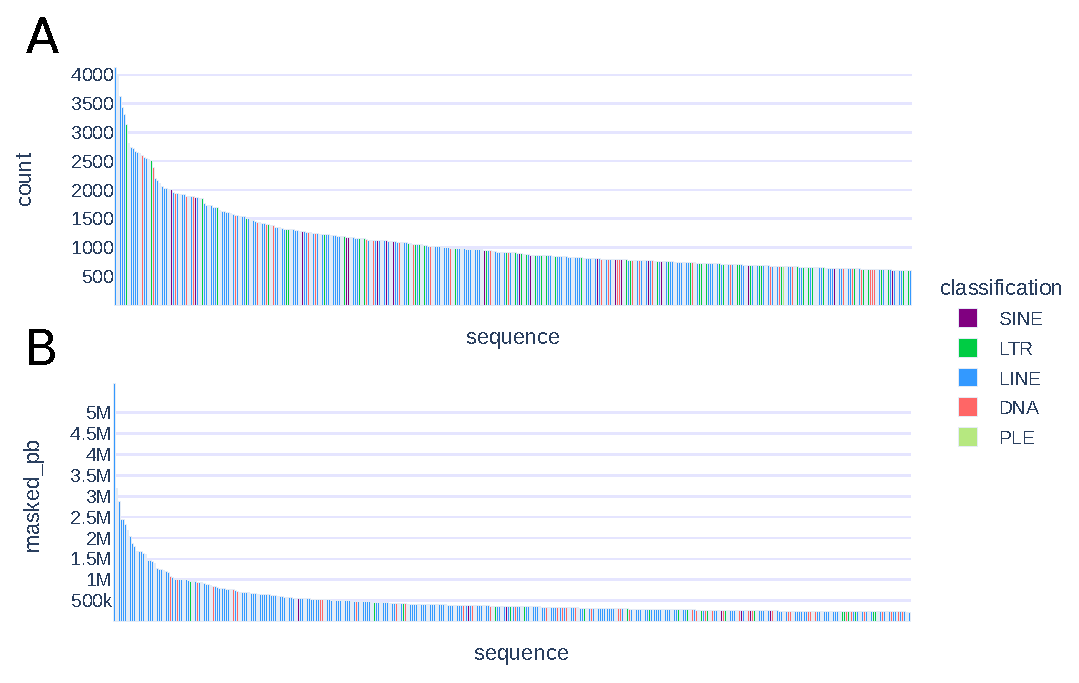
\includegraphics[width=\textwidth]{img/plots/rep_mask.eps}
    \caption{Graphique montrant les familles plus présentes sur le génome d'\textit{Ae. albopictus}.}
    \caption*{
    \scriptsize{
    \textbf{A} - Distribution des \acrlong{et} les plus répétés. Chaque barre représente une séquence de notre librairie; en ordonnée: le nombre de fragments identifié par \texttt{RepeatMasker}. \textbf{B} - En ordonnée: le nombre de bases masquées. 
    }}
    \label{fig:rep_mask}
\end{figure}

\bigskip

Pour quantifier exactement les proportion de chaque classe d'\acrshort{et}, on a exécuté une dernière fois \texttt{RepeatMasker}. Les résultats obtenus sont montrés dans \tableautorefname{ \ref{tab:rm_quantif}}. On peut observer que comme dans les annotations d'autres auteurs (\tableautorefname{ \ref{tab:annot_state_of_art}}), la catégorie d'\acrshort{et} qui s'impose sur le génome est la classe I (rétrotransposons) avec un abondant 39.43\% du génome. Parmi les éléments de classe I, on distingue particulièrement les \acrshort{line} et les \acrshort{ltr}. \\ 
Les \acrlong{et} de classe II couvrent le 16\%, quantité qui est très similaire à les annotations précédentes. On peut ainsi apprécier l'effort réalisé par les outils \textit{de novo} dans la détection des \acrshort{ltr} (en particulier \texttt{RepeatModeler2}, qui par rapport à sa version précédente a intégré des modules dédiés à leur détection). \\

En \figureautorefname{ \ref{fig:pie_chart}}, on montre une représentation graphique du paysage des éléments répétés d'\textit{Ae. albopictus}. On peut observer comme les \acrshort{line}, les \acrshort{ltr} et les ADN occupent de manière presque équivalente le génome. \\
Parmi les \acrshort{line}, les super-familles les plus représentées sont \textit{R1}, \textit{RTE} et \textit{JAM1}.  Parmi les \acrshort{ltr}, on retrouve principalement les super-familles \textit{Bel-Pao}, \textit{Copia} et \textit{Gypsy}. Chez les ADN, on retrouve les super-familles \textit{hAT} et \textit{Sola}, mais on peut observer la difficulté des outils de classification à classifier ces éléments; en fait la majorité des séquences a été classifiée uniquement comme ADN car un consensus au niveau suivant (super-famille ou famille) n'a pas été trouvé. \\

\bigskip

\begin{table}[H]
    \centering
    \begin{tabular}{r|c|c|c}
        \toprule
        \textbf{Classe} & \textbf{Nb d'instances} &  \textbf{Nb de bases masqués} (pb) & \textbf{\% du génome}\\
        \midrule
        \rowcolor{gray!10} 
        \textbf{Classe I} & 1 823 774 & 571 983 224 & 39.43 \\
        dont \acrshort{sine} & 91 912 & 16 750 947 & 1.15 \\
        \rowcolor{gray!10}
        dont \acrshort{line} & 953 856 & 301 852 752 & 20.81 \\
        dont \acrshort{ltr} & 778 006 & 253 379 525 & 17.47 \\
        \rowcolor{gray!10}
        \textbf{classe II} & 825 697 & 232 145 026 & 16.00 \\
        \textbf{Non-classifiées} & 149 610 & 58 788 174 & 4.05 \\
        \midrule
        \textbf{Total} & 2 799 081 & 862 916 424 & 59.49 \\
        \bottomrule
    \end{tabular}
    \caption{Quantification des \acrlong{et} dans le génome d'\textit{Ae. albopictus}.}
    \label{tab:rm_quantif}
\end{table}

\bigskip

\begin{figure}[H]
    \centering
    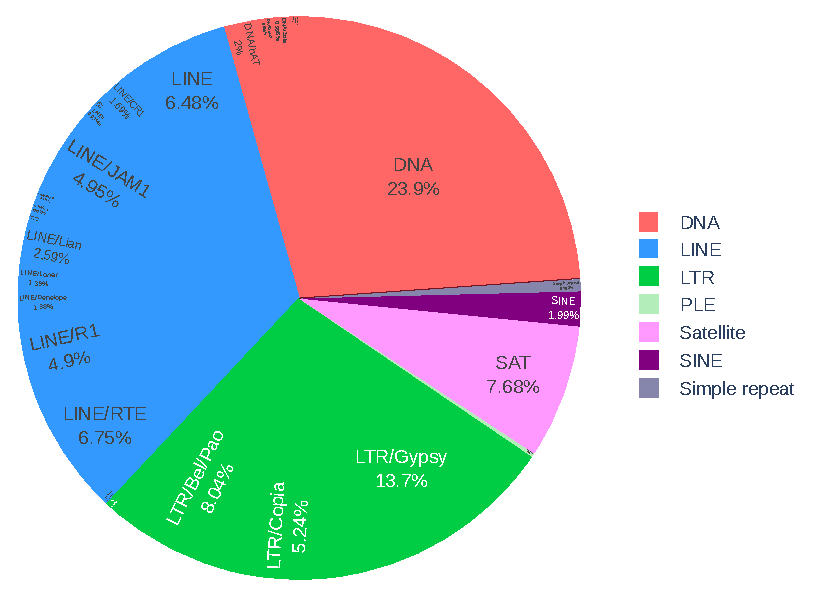
\includegraphics[width=0.9\textwidth]{img/plots/pie_chart.eps}
    \caption{Représentation graphique du contenu en \acrshort{et} d'\textit{Ae. albopictus}.}%TODO: à finir
    \label{fig:pie_chart}
\end{figure}

\clearpage\newpage

\section{Conclusion et perspectives}\label{sec:concl}

\paragraph{L'annotation} Cette étape, qui a été particulièrement intense d'un point de vue de temps de calcul, a été indispensable pour la construction de la librairie finale. Dans le document, on a montré l'intérêt (\subsectionautorefname{ \ref{sec:clustering_and_refining}} - \textsc{\nameref{sec:clustering_and_refining}}) d'utiliser un double approche homologie-\textit{de novo}. On a pu noter que, d'une part l'utilisation d'un approche par homologie est indispensable pour avoir un ensemble d'éléments fiable et que, d'autre part, un approche \textit{de novo} est nécessaire pour l'identification de nouvelles familles (\figureautorefname{ \ref{fig:contribution}}). \\
Le jeu de 59 848 séquences obtenu a été traité par la suite dans la construction de la librairie. \\


\paragraph{Construction de la librairie} La construction d'une librairie d'\acrshort{et} est une analyse qui aujourd'hui est loin d'être standardisée. Il en est la preuve le fait que très souvent celle-ci consiste uniquement dans une première étape d'annotation (généralement en utilisant seulement un approche par homologie, ex. avec \texttt{RepeatMasker}) et une deuxième étape de classification. Cela permet, bien sur, d'avoir une librairie utilisable dans les analyses \og downstream \fg{}, mais qui sera ainsi difficilement complète et soignée. Ici, on a essayer de décrire de la meilleure façon possible le paysage des \acrlong{et} d'\textit{Ae. albopictus}. \\
Retravailler les copies obtenues à partir des consensi (\subsectionautorefname{ \ref{get_copies}} - \textsc{\nameref{get_copies}}) générées par les outils d'annotation a permis de gérer aisément la redondance des séquences, en utilisant des outils de masquage du génome (comme \texttt{RepeatMasker} dans notre cas) et de clustering (\texttt{cd-hit-est}). \\
Il a aussi permis de vérifier le support génomiques des consensi (comme montre en \tableautorefname{ \ref{tab:nb_not_matching_tab}}) ainsi que de réunir de manière plus parcimonieuse l'information apportée par les différents outils (en re-appelant des consensi à l'aide de \texttt{Refiner}). \\

La méthodologie utilisée peut cependant, être discutable sous plusieurs points de vue. Par exemple, au niveau du seuil stringent utilisé (\autoref{repeatmasker}) pour \texttt{RepeatMasker} pour récupérer les fragments correspondants aux consensi, une utilisation d'un seuil plus faible aurait permis une détection plus vaste d'éléments; mais tout comme pour le sous-échantillonnage des séquences lors de l'appel des consensi (lors de l'utilisation de \textit{Refiner}), il s'agit d'une contrainte technique liée au temps de calcul, de difficile résolution. \\
De même, on aurait pu préférer de filtrer les fragments obtenus en fonction de la longueur, après utilisation d'\texttt{\acrshort{octfta}}, mais cela aurait demandé un temps de calcul supplémentaire. \\
On reconnaît aussi la limite technique portée par \texttt{cd-hit-est} dans le clustering de séquences plus ou moins divergées, lequel pour avoir un résultat satisfaisant a demandé d'effectuer plusieurs clustering de suite. \\
Le nombre total de séquences obtenus suite à la construction de la librairie a été de 23 009. \\


\paragraph{Axes d'amélioration pour le pipeline sur le polissage} Bien que le pipeline a été capable de fournir des résultats valables pour notre expérience, il peut être encore développé sur plusieurs aspects. \\
Par exemple, on peut imaginer d'implémenter une fonction permettant d'étendre de façon plus efficace les extrémités du consensus (certaines séquences sont bien étendues mais parfois les extrémités sont moins \og lissés \fg{} que dans des autres cas) en faisant des ajustement sur les paramètres en fonction des observations empiriques. \\
Jusqu'à maintenant, on n'a pas pris en compte dans le programme l'augmentation des fragments comme critère pour trancher entre la séquence de l'itération \textit{i} avec celle de l'itération \textit{i-1}. De même on pourrait imaginer de prendre en compte les \acrshort{orf} et, de donner des poids différents aux domaines protéiques détectés selon qu'ils soient trouvé dans le même sens que le consensus ou en anti-sens.  \\
Le jeu de données utilisé pour le test contenait une majorité de séquences provenant de l'ordre \acrshort{ltr}, donc il serait intéressant de tester le pipeline sur une jeu de données plus hétérogène. \\
Enfin, on pourrait également imaginer de concevoir une idée meilleure pour gérer la sur-extension des solo-\acrshort{ltr} (en tenant compte de la similarité des régions flanquantes rajoutées à chaque itérations) et de tester les séquences marquées comme \acrshort{ssr} (par exemple en essayant de les classifier pour voir si effectivement il ne s'agit pas de faux positifs). \\


\paragraph{La classification} La classification des \acrlong{et} est une étape cruciale qui permet de connaître la composition en \acrshort{et} du génome analysé. Celle-ci est fortement dépendante de la qualité des bases de données utilisées; si la base de données manque de certaines catégories d'\acrshort{et}, ceux-ci seront peu, voire pas du tout, classifiés. Aujourd'hui \texttt{RepBase} est ce qu'il y a de plus complet en termes de bases de données pour les \acrlong{et}. Malgré l'utilisation de celle-ci, on a pu remarquer une problématique liée à la classification de certain éléments non-autonomes non représentés, notamment comme les \acrshort{mite}, auxquels on a dédié beaucoup de temps lors de l'annotation avec l'utilisation de \texttt{MITE-Tracker}. \\
Comme perspective pour en améliorer la classification, on propose de classifier manuellement quelques séquences de \acrshort{mite} (ainsi que d'autre catégories pour lesquelles on souhaite améliorer la classification) et, de les joindre à la base de données utilisée pour la classification. \\

On souhaite également signaler une difficulté globale dans la classification provoquée par une utilisation non unifiée et cohérente des conventions de nomenclature des \acrshort{et}  au sein des différentes bases de données ainsi que des différents outils de classification. Très souvent, la hiérarchie et la nomenclature proposée par \textit{Wicker et al.} \cite{wicker}, laquelle représente à ce jour le standard pour la classification des \acrshort{et}, est rarement respectée dans sa globalité. Pour faire un exemple, dans la plupart des outils de classification, les éléments de classe II notés comme DNA, sont directement comparés à les super-familles des \acrshort{line} ou des \acrshort{sine} ou encore à l'ordre des \acrshort{ltr} (pour plus de détail sur la hiérarchie des \acrshort{et}, se référer à la \figureautorefname{ \ref{fig:classif_et}}). \\
Pour simplifier et, dans un premier temps permettre une classification homogène entre les différentes outils de classification utilisés dans cet étude, on a préféré d'utiliser une nomenclature \og faussée \fg{}; on propose donc parmi les perspectives, de réaliser une meilleure classification, respectant la hiérarchie proposée par \textit{Wicker et al.}, sans aucune exception. \\

Dans la librairie finale, on a choisi de ne garder pour le moment, que les 5 465 consensi ayant reçu une classification. \\
On propose ainsi, effectuer une analyse plus fine sur les consensi qui restent ($23 009 - 5 465 = 17 544$); en particulier, en rajoutant une étape de classification structurelle pour permettre une meilleure détection des éléments comme les \acrshort{tir} et les \acrshort{mite} (lesquels présentent des \textit{\acrlong{tir}}, qui sont facilement identifiables); d'effectuer un \texttt{blastx} (blast de l'ADN traduit dans les six cadres de lecture possible) contre une base de données (ex. \texttt{nr}) de domaines protéiques issus de gènes pour pouvoir exclure toute séquence pouvant être un gène (provenant d'\textit{Ae. albopictus} mais aussi d'insertions virales ou de contaminations lors du séquençage du génome). \\

\bigskip

En conclusion, lors de ce stage nous avons construit une librairie d'\acrlong{et} d'\textit{Aedes albpictus} en tenant compte des exigences qu'elle devait respecter; à savoir l'exhaustivité (pouvoir décrire la totalité du paysage d'\acrshort{et} du génome) et l'intégralité des séquences elles-mêmes (en vue du génotypage sur le projet 1000 génomes). \\
Juger de l'exhaustivité d'une annotation n'est jamais une tâche simple, mais en comparaison avec les annotations antérieures (\tableautorefname{ \ref{tab:annot_state_of_art}}), nous avons démontré qu'une dualité entre une approche par homologie et \textit{de novo} peut apporter de l'information supplémentaire par rapport aux deux approches utilisées séparément. Par conséquence, notre librairie permet de masquer 59.49\% du génome, contre le 55.81\% de l'annotation de \textit{Palatini et al,} 2020 , dans les deux cas le même assemblage a été utilisé en donnant des résultats qui peuvent être comparés. \\
L'intégralité des séquences est peut être encore plus difficile à évaluer, malgré cela la méthode développée a donné des résultats satisfaisants. (\sectionautorefname{ \ref{sec:polish}} - \textsc{\nameref{sec:polish}}). \\
Au niveau du paysage des \acrshort{et}, nous avons pu re-confirmer que la catégorie d'éléments la plus large en termes de proportion génomique (301Mpb) et de nombre de copies (953 856 instances totales) sont les \acrshort{line}s (rétrotransposons)  lesquels représentent 20.81\% du génome. Parmi les \acrshort{line}s nous avons pu retrouver des nombreuses familles déjà décrites chez les moustiques \cite{tu_structural_1998, biedler_non-ltr_2003, boulesteix_transposable_2005}, comme \textit{RTE}, \textit{R1}, \textit{Lian} et \textit{Loner}. Nous retrouvons également des proportions assez similaires pour les \acrshort{ltr} et les ADN, avec respectivement 17.47\% et 16.00\% de couverture sur le génome.




\newpage

\newgeometry{top=2cm,bottom=3cm,right=1.5cm,left=1.5cm}
\setlength{\columnsep}{0.5cm}
\twocolumn

\phantomsection
\printbibliography % Prints bibliography
\addcontentsline{toc}{section}{Références} % add to the content table


\nocite{python3}
\nocite{perl}
\nocite{gnu2007free}
\nocite{benson_tandem_1999}
\nocite{noauthor_ucsc_nodate}
\nocite{neph_bedops_2012}
%\nocite{katoh_mafft_2002}
\nocite{fu_cd-hit_2012}
\nocite{noauthor_ninja_nodate}
%\nocite{camacho_blast_2009}
\nocite{mistry_challenges_2013}
\nocite{rognes_vsearch_2016}
\nocite{chapman_biopython_2000}
\nocite{noauthor_numpy_nodate}
\nocite{mckinney_pandas_nodate}
%\nocite{bailly-bechet_one_2014}
\nocite{parisot_transposable_2021}
%\nocite{tange_2022_6213471}
%\nocite{schloss_introducting_2009}
\nocite{quinlan_bedtools_2010}
%\nocite{girgis_identity_2021}
\nocite{li_lh3seqtk_2022}
\nocite{xu_ltr_finder_2007}
\nocite{ou_ltr_finder_parallel_2019}
\nocite{su_tir-learner_2019}
\nocite{shi_generic_2019}
\nocite{xiong_helitronscanner_2014}
\nocite{zhang_tesorter_2019}
% \nocite{noauthor_babraham_nodate}
% \nocite{noauthor_genomics_nodate}

\newpage

\newgeometry{top=2cm,bottom=3cm,right=1cm,left=1cm}

\phantomsection
\newcounter{supplementarsection}
\renewcommand{\thesupplementarsection}{Annexes}
\refstepcounter{supplementarsection}
\label{s:annexes}
\section*{Annexes}
\addcontentsline{toc}{section}{Annexes} % add to the content table

\beginsupplement

\begin{figure}[H]
    \centering
    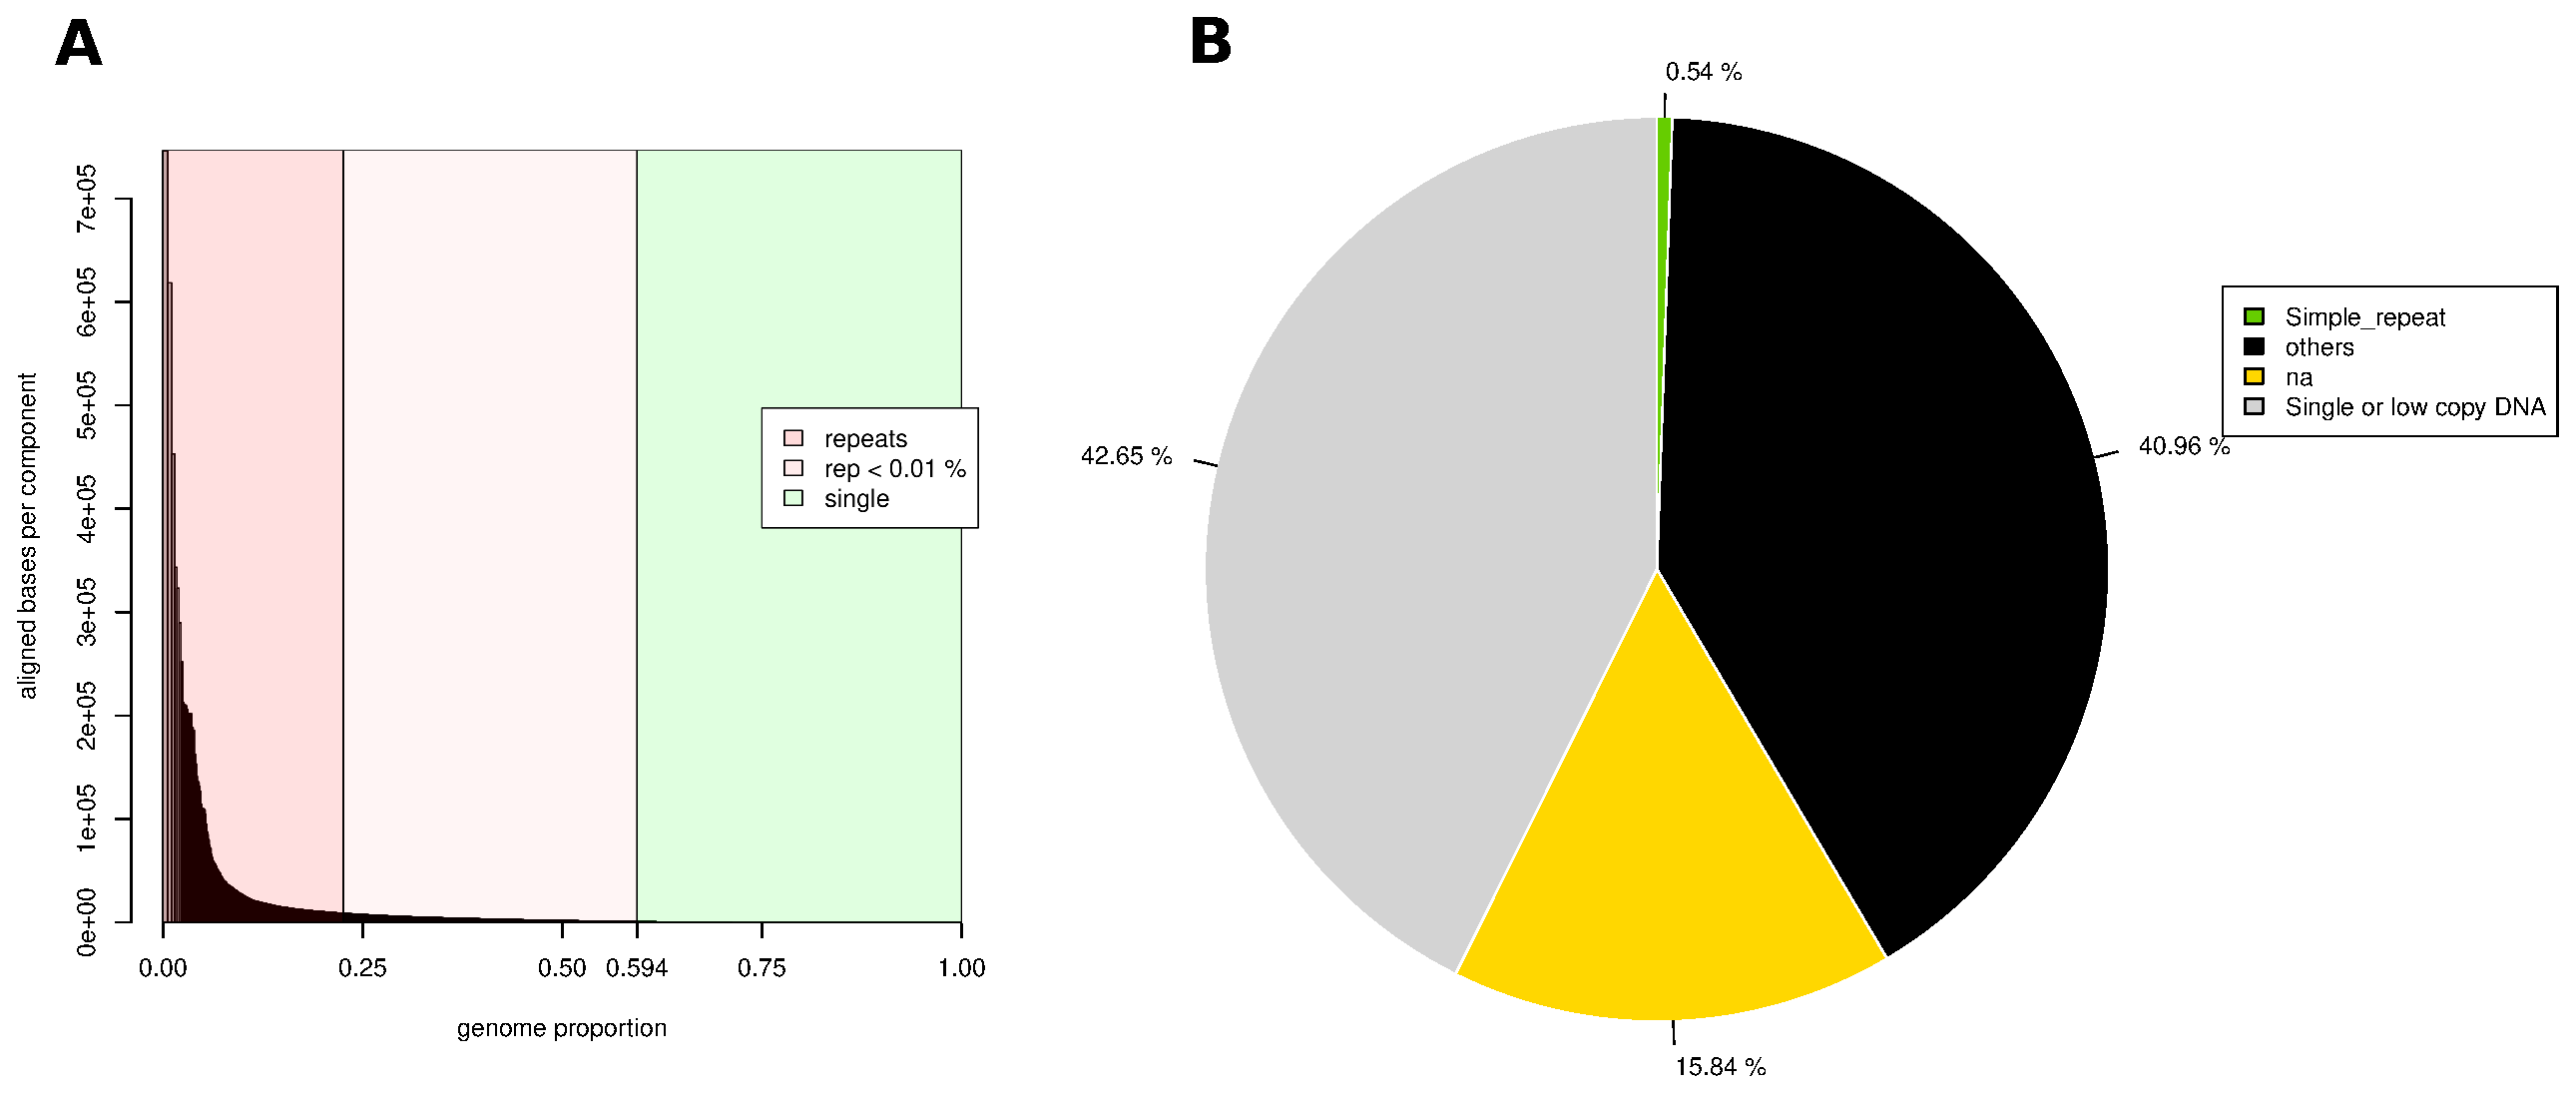
\includegraphics[width=0.8\textwidth]{img/plots/repbase_realsize.eps}
    \caption{Estimation de la fraction répétée sur un jeu de données réel.}
        \caption*{\scriptsize

    \textbf{A} - \textbf{Nombre des bases alignés par composante en fonction de la proportion génomique.} En rouge, la fraction génomique fortement répétée; en lilas, la fraction normalement répétée et enfin, en vert l'ADN non répété. \textbf{B} - \textbf{Estimation de la composition en \acrlong{et}.} \`A différence de la \figureautorefname{ \ref{fig:coverage_simulated}}, ici on obtient la grande tranche noire (correspondant aux éléments identifiés) car la librairie utilisée (\texttt{RepBase}), n'est pas formaté de la même manière que la librairie proposée par défaut dans \texttt{dnaPipeTE}.}
    \label{fig:repbase_realsize}
\end{figure}

\begin{figure}[H]
    \centering
    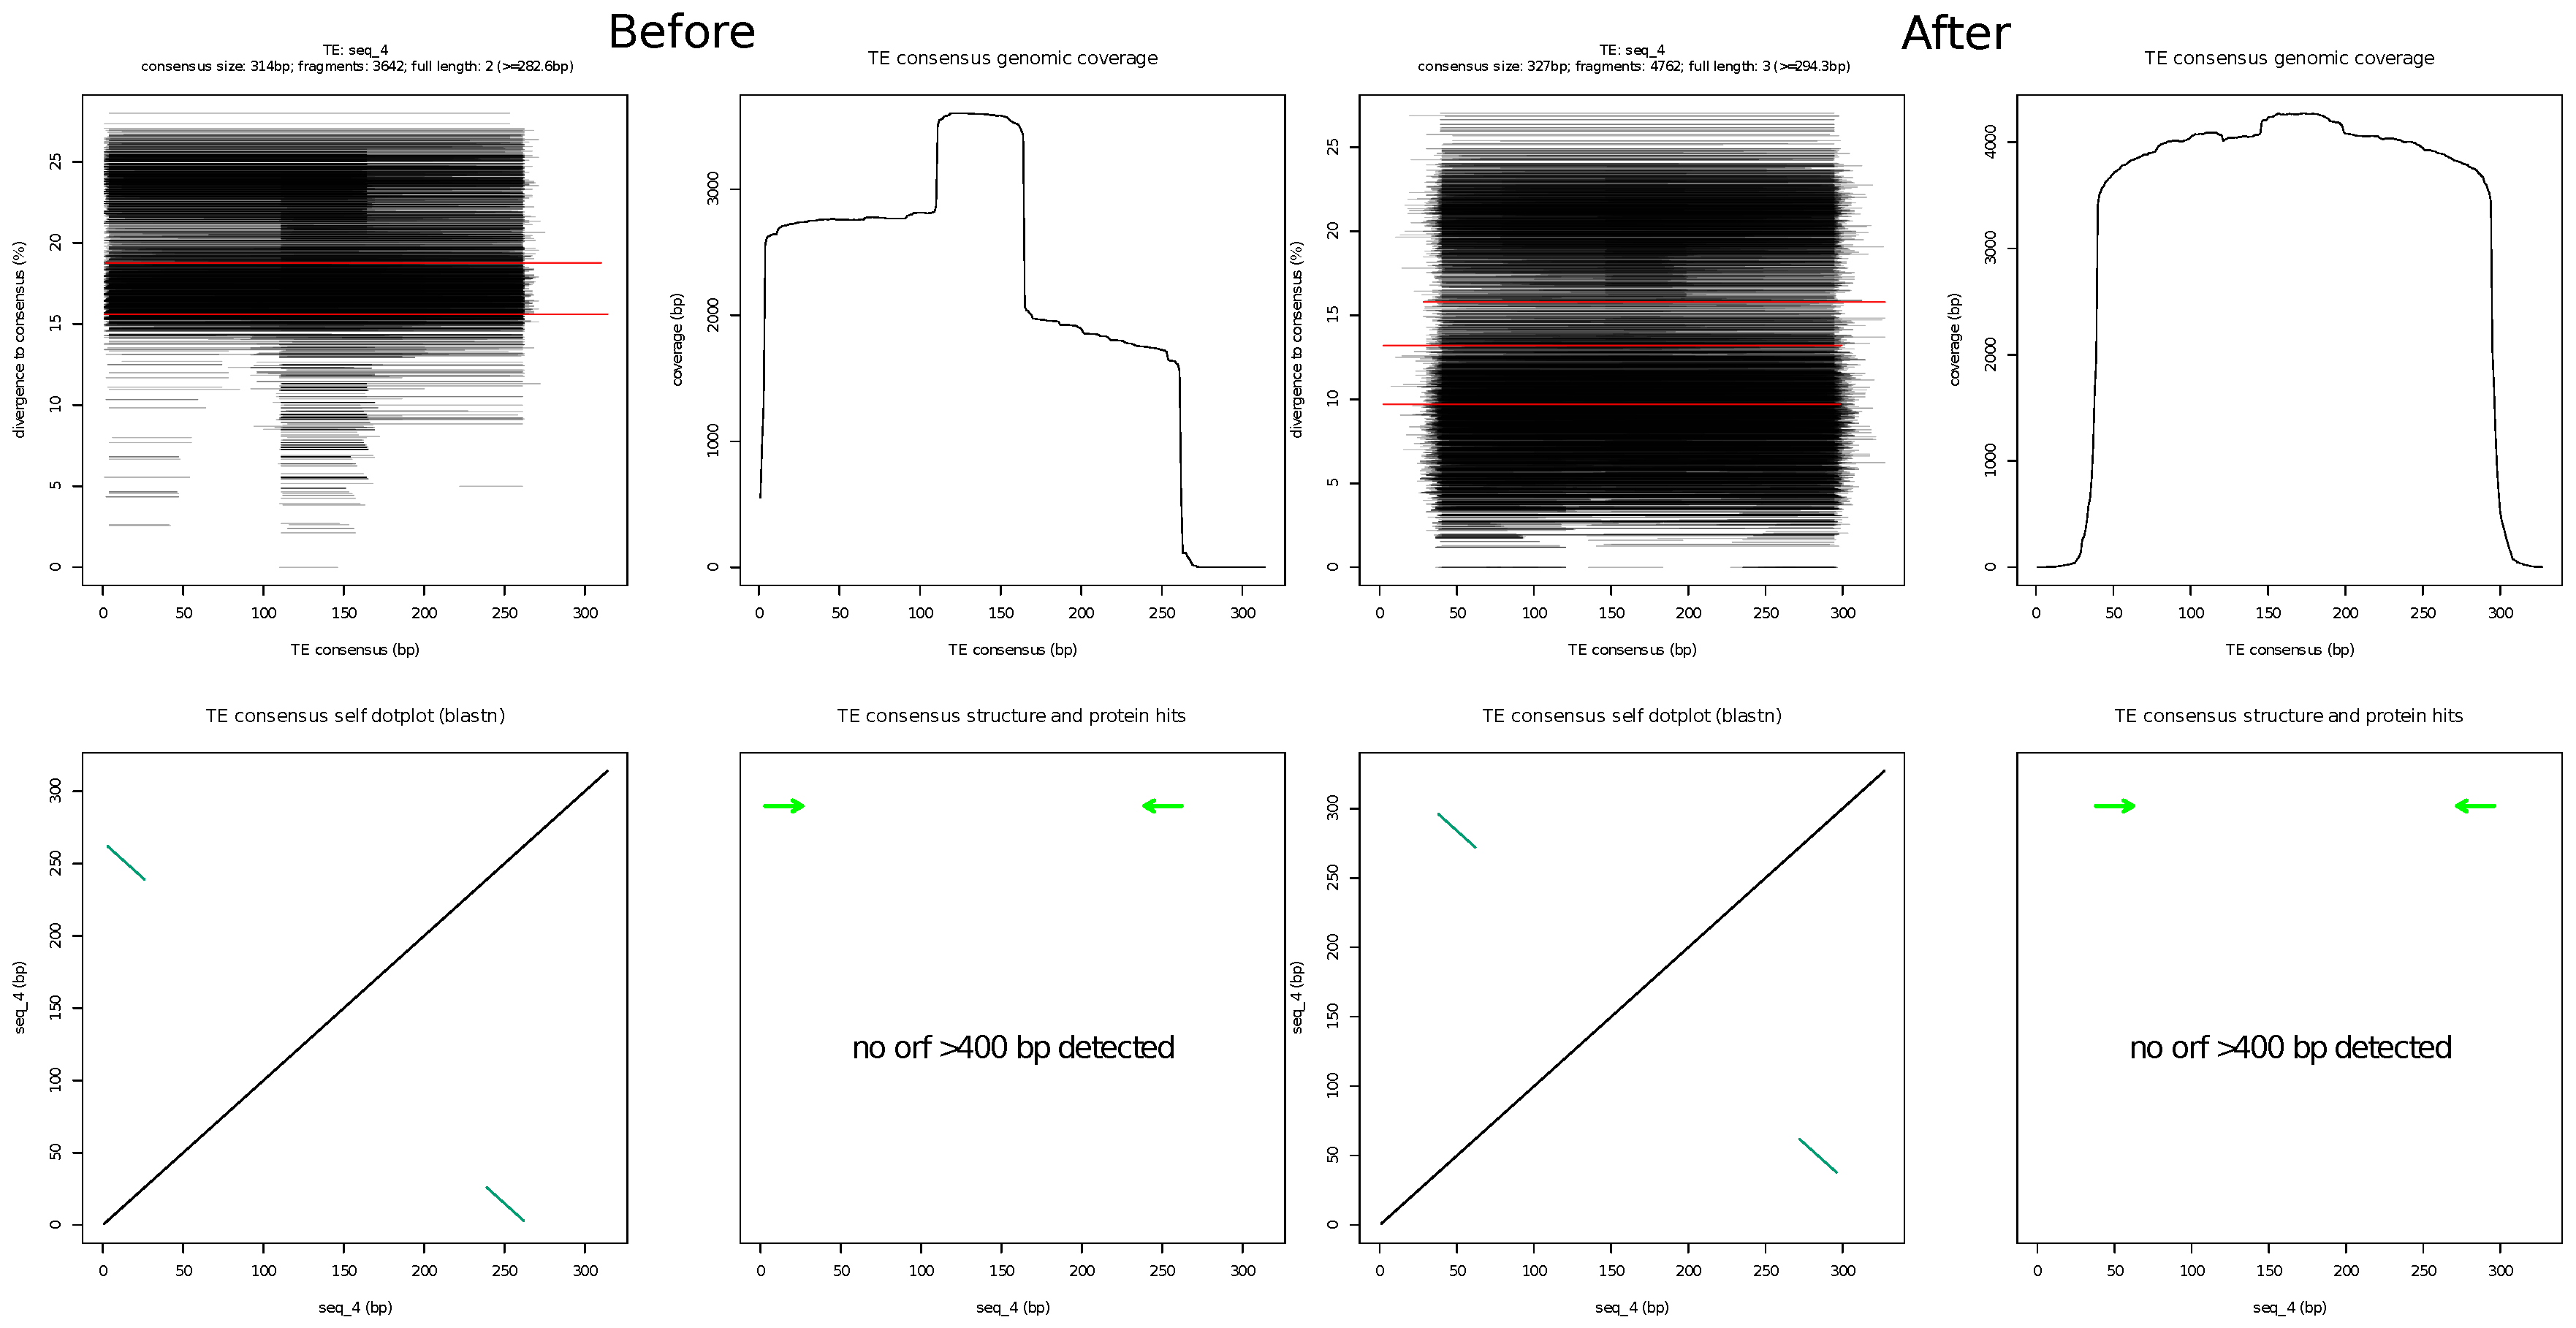
\includegraphics[width=\textwidth]{img/plots/seq_4.eps}
    \caption{Séquence 4.}
    \label{fig:seq_4}
\end{figure}

\begin{figure}[H]
    \centering
    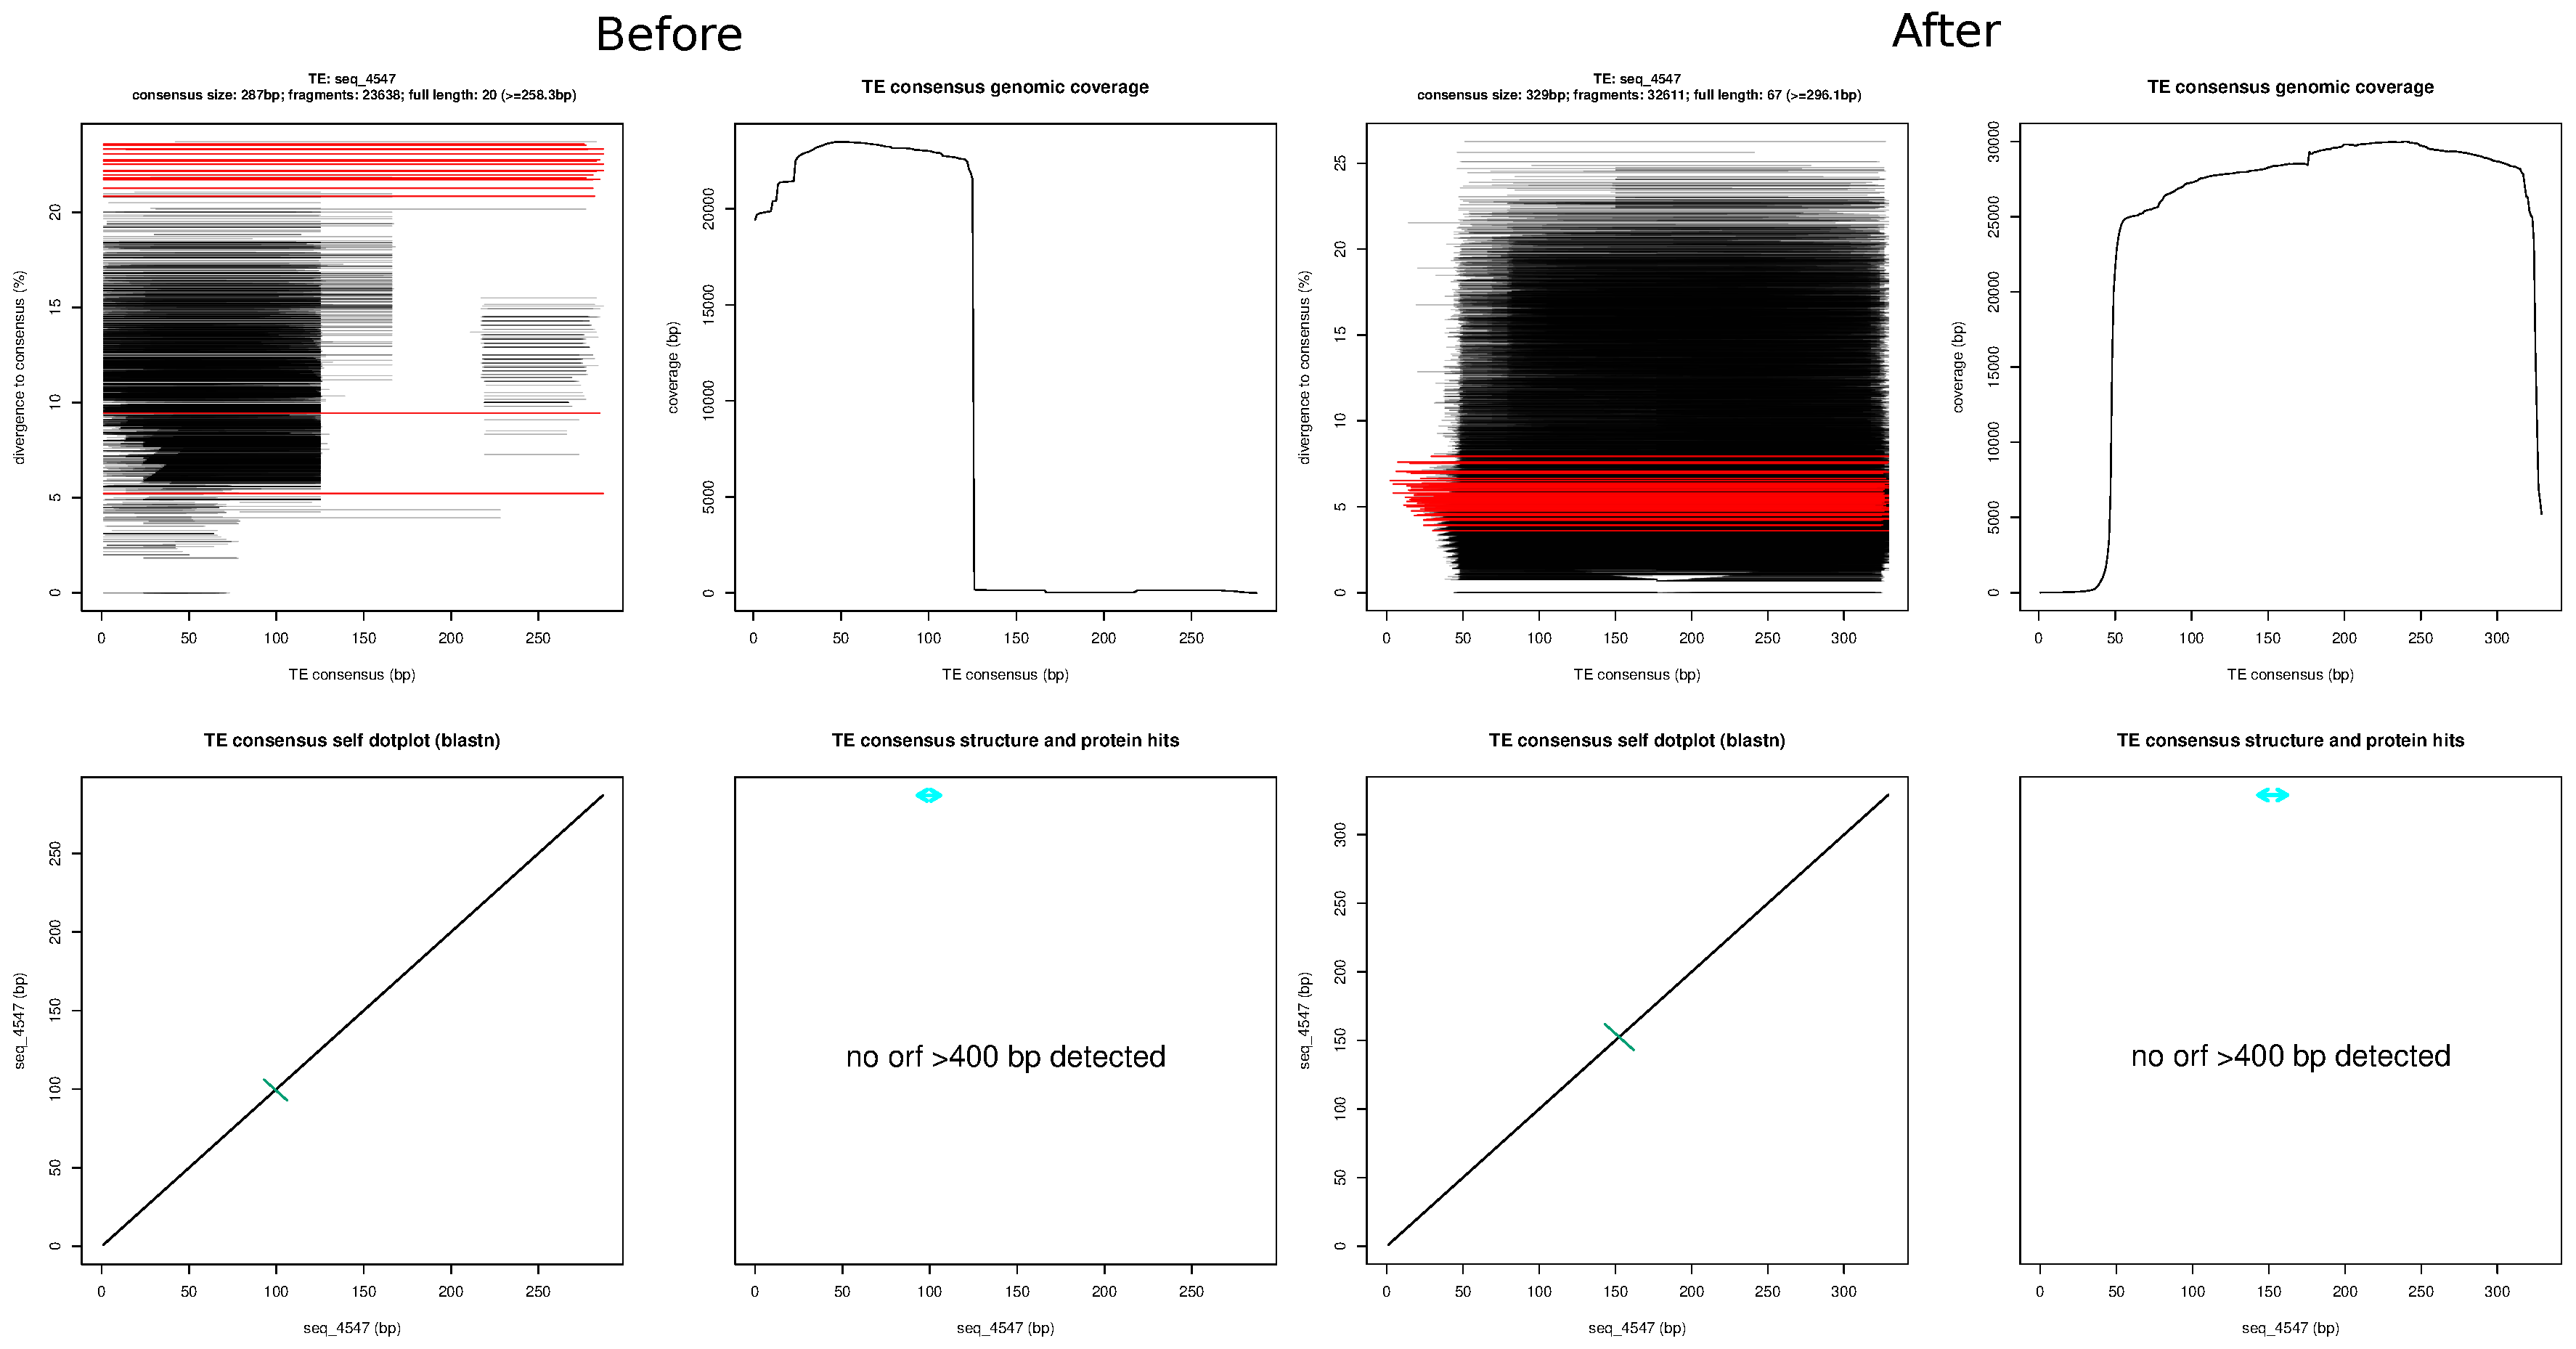
\includegraphics[width=\textwidth]{img/plots/seq_4547.eps}
    \caption{Séquence 4547.}
    \label{fig:seq_4547}
\end{figure}

\begin{figure}[H]
    \centering
    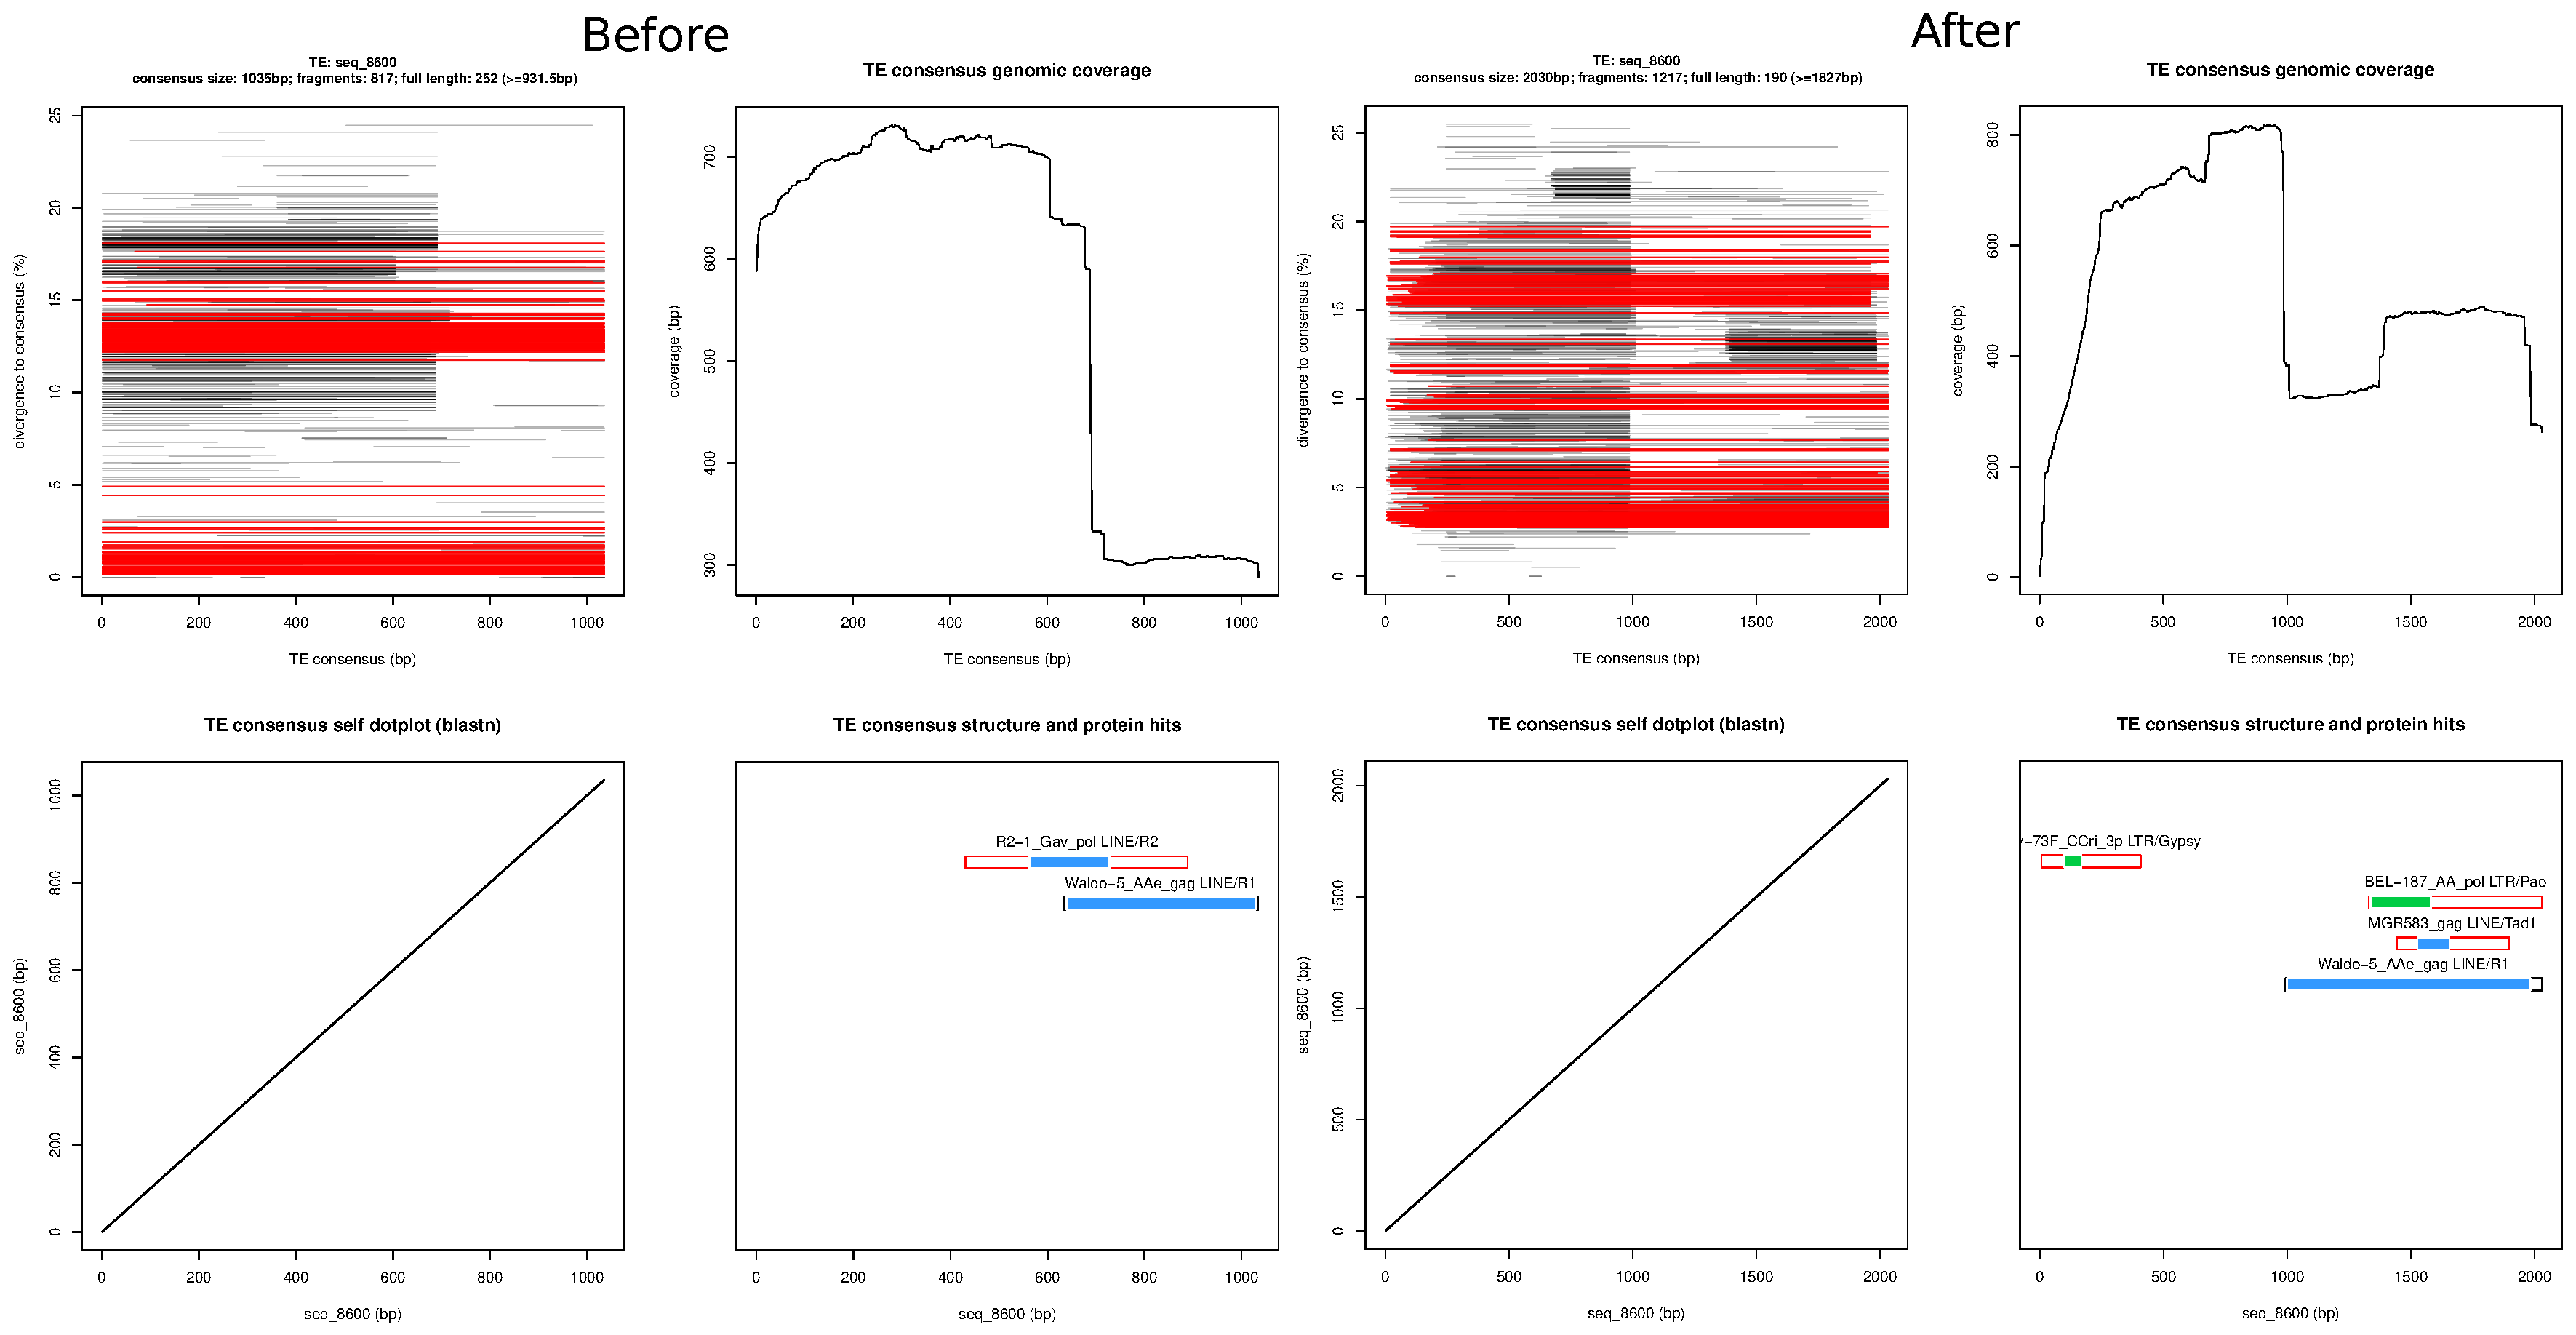
\includegraphics[width=\textwidth]{img/plots/seq_8600.eps}
    \caption{Séquence 8600.}
    \label{fig:seq_8600}
\end{figure}

\begin{figure}[H]
    \centering
    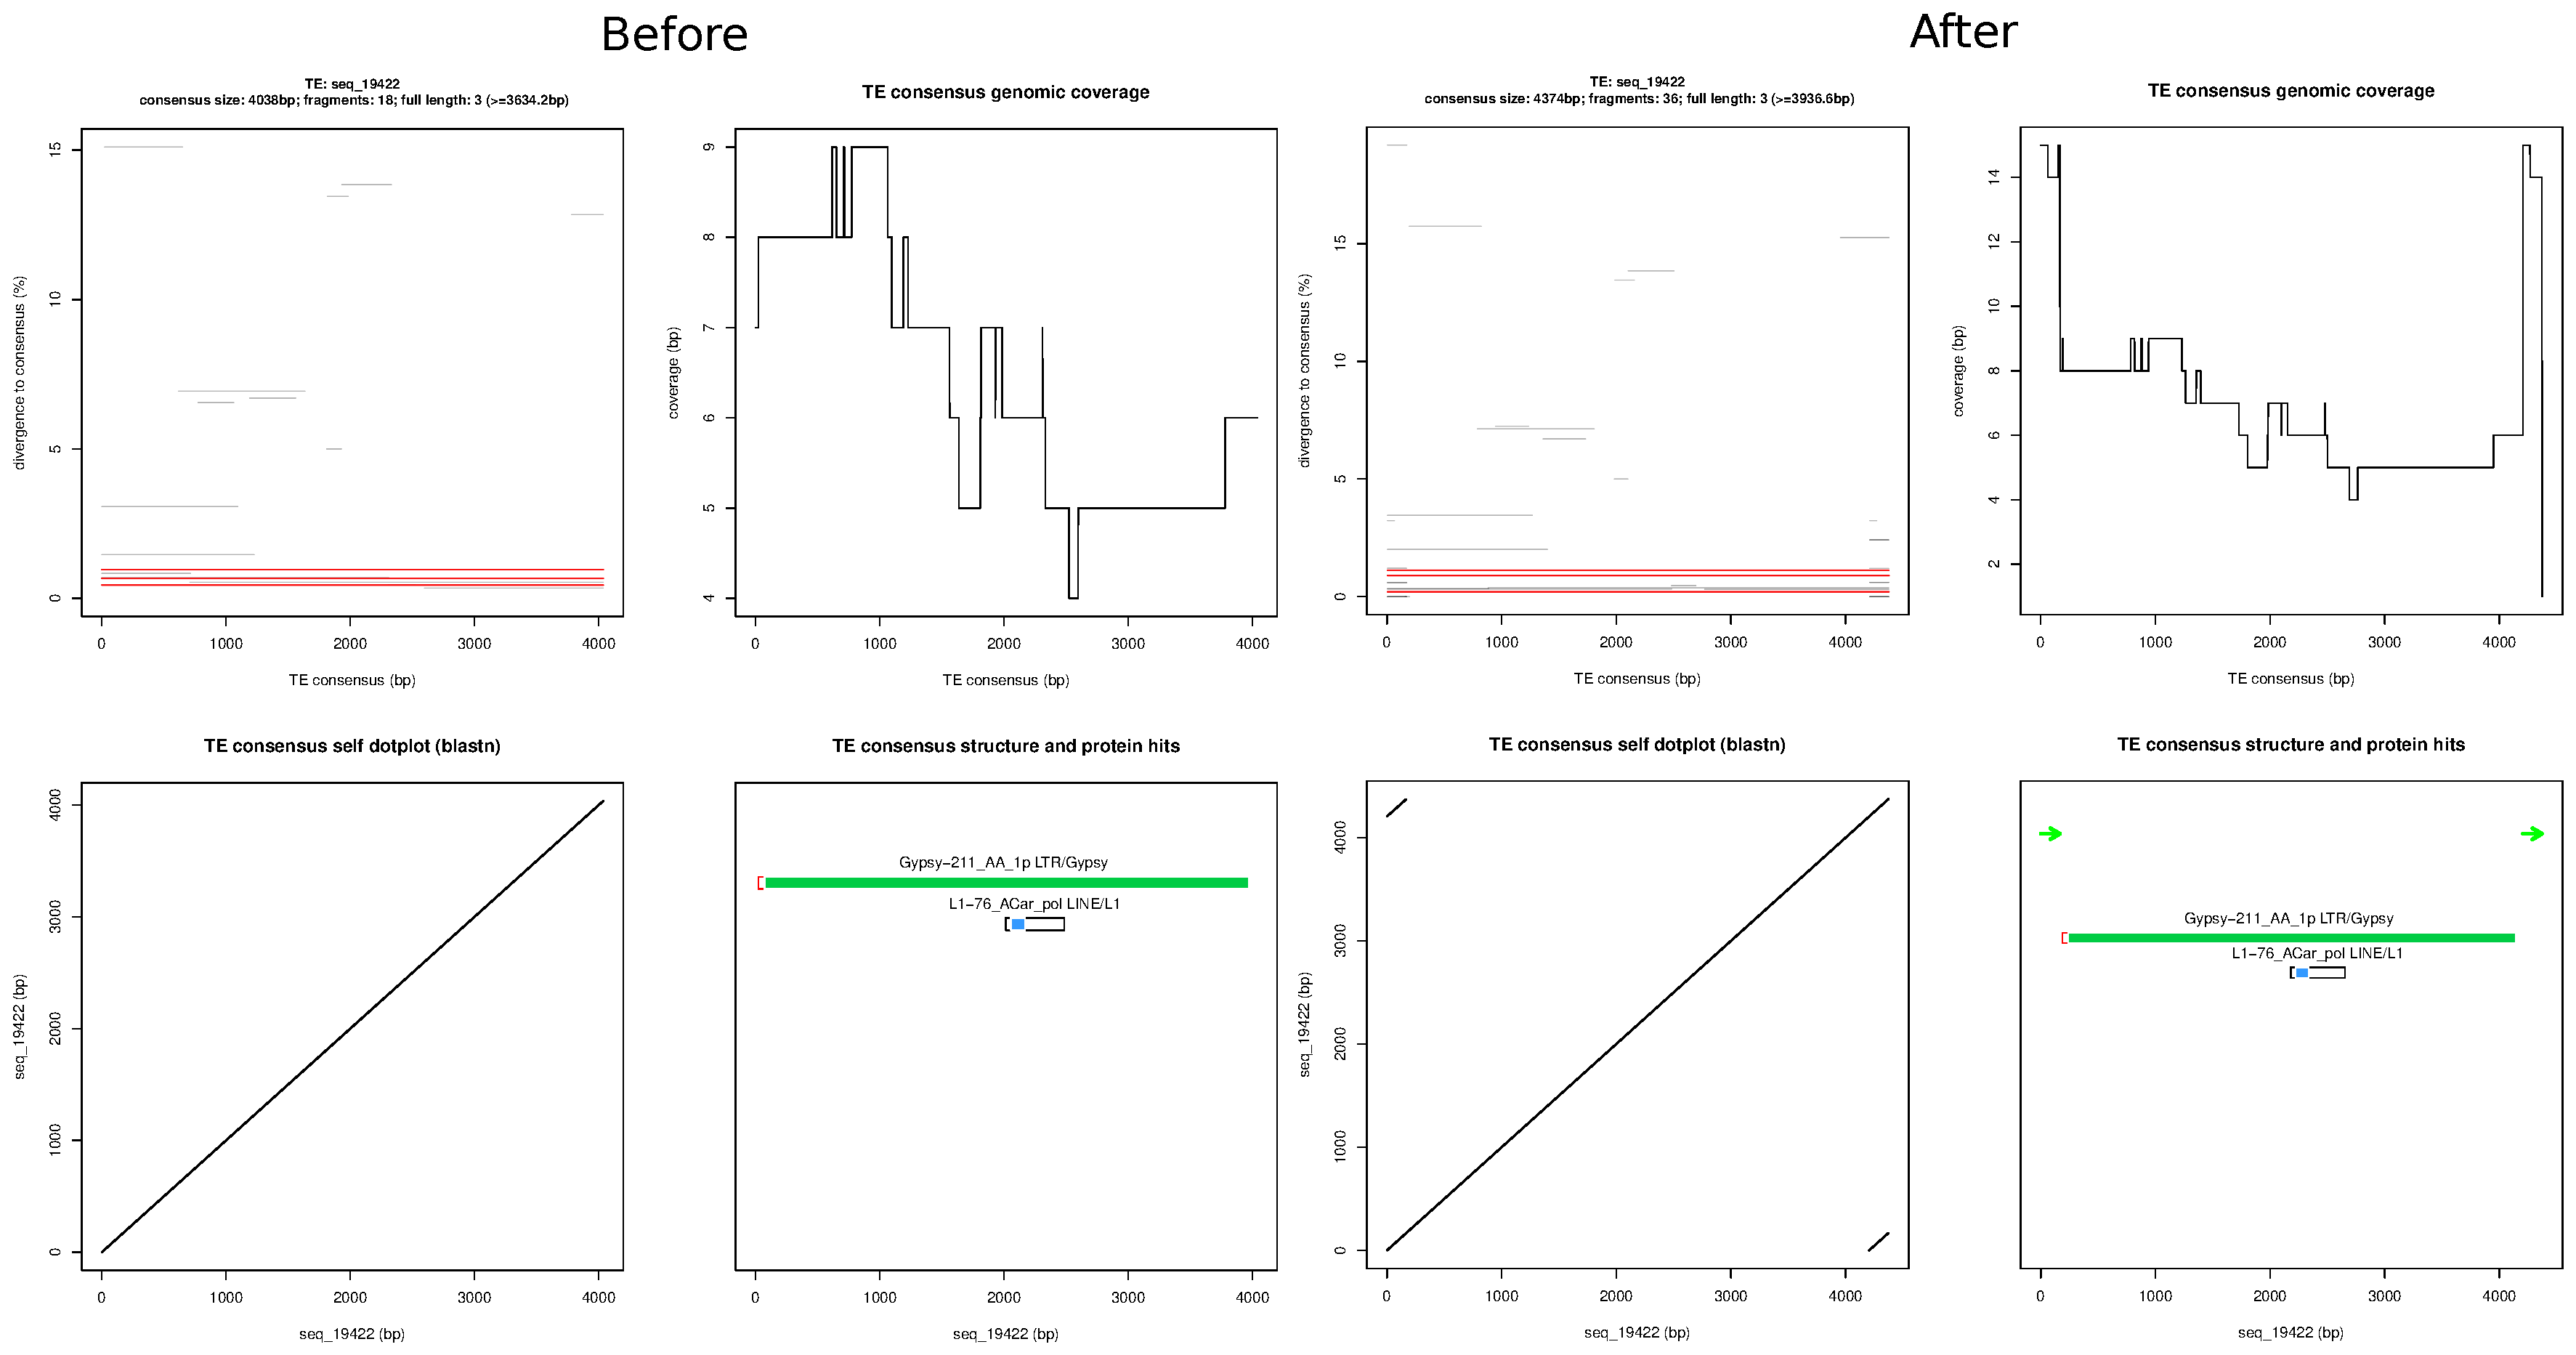
\includegraphics[width=\textwidth]{img/plots/seq_19422.eps}
    \caption{Séquence 19422.}
    \label{fig:seq_19422}
\end{figure}

\bigskip

\begin{table}[h]
    \begin{tabular}{|r|c|c|c|c|c|c|}
        \hline
         & \textbf{\makecell{Date de \\ publication}} & \textbf{\makecell{GenBank \\ accession}} & \textbf{\makecell{Méthode \\ d'assemblage}} & \textbf{\makecell{Longueur \\ totale}} & \textbf{\makecell{Téchnologie de \\ séquençage}} \\
        \hline\hline
        \textit{Chen et al.} & 23/02/2016 & GCA\_001444175.2 & \texttt{SOAPdenovo - v2.04} & 1 923 476 627 & \texttt{Illumina HiSeq 2000} \\
        \hline
        \textit{Palatini et al.} & 28/06/2019 & GCA\_006496715.1 & \texttt{Canu - v1.7} & 2 538 387 871 & \texttt{PacBio Sequel} \\
        \hline
        \textit{Boyle et al.} & 20/04/2021 & GCA\_018104305.1 & \texttt{\makecell{Lep-Anchor \\ v. March-2020}} & 1 450 641 013 & PacBio \\
        \hline
    \end{tabular}
    \vspace{0.3cm}\newline
    \begin{tabular}{|r|c|c|c|}
        \hline
         & \textbf{\makecell{Nb de \\ scaffold}} & \textbf{\makecell{N50 \\ scaffold}} & \textbf{\makecell{L50 \\ scaffold}}  \\
        \hline\hline
        \textit{Chen et al.}  & 154 782 & 201 017 & 2 851 \\
        \hline
        \textit{Palatini et al.} & 2 197 & 55 702 539 & 13 \\
        \hline
        \textit{Boyle et al.} & 574 & 10 094 208 & 43 \\
        \hline
    \end{tabular}
    \caption{Comparaison des différents assemblages génomiques d'\textit{Ae. albopictus} déposés sur le NCBI.}
    \label{tab:assembly_comparaison}
\end{table}

\bigskip
\clearpage

\begin{lstlisting}[language=bash, frame=trb, caption=Commandes \texttt{RepeatModeler2}., label=RM2]
# BuildDatabase generate a database for a given reference genome, it is installed with RepeatModeler2
BuildDatabase -name Aalb $DATA_DIR/GCA_006496715.1_Aalbo_primary.1_genomic.fna

# NINJA_DIR: path to folder containg binaries for NINJA
# the export is needed to avoid this error https://github.com/Dfam-consortium/RepeatModeler/issues/134
export $NINJA_DIR

RepeatModeler -database Aalb -pa $nb_cpus -LTRStruct
\end{lstlisting}  

\vspace{0.5cm}

\begin{lstlisting}[language=bash, frame=trb, caption=Commandes \texttt{EDTA}., label=edta]
# activation of the conda environment provided by the author
conda activate EDTA

# EDTA needs header with length shorter than 13 characters
awk -F " " '{ if ($0 ~ /^>/) { print ">"$6;} else { print $0}}' GCA_006496715.1_Aalbo_primary.1_genomic.fna  | sed -e 's/,//' > GCA_006496715.1_Aalbo_primary.1_genomic.short_header.fna


# run of EDTA_raw.pl for each transposable elements type (ltr|tir|helitron)
perl $EDTA_DIR/EDTA_raw.pl --genome $DATA_DIR/GCA_006496715.1_Aalbo_primary.1_genomic.short_header.fna --type ltr|tir|helitron --overwrite 0 -t $nb_cpus 
# --overwrite 0: it allows to merge results from differents runs without deleting the results previously obtained

# merging and finalising the annotation, it must be run in the same folder as previously commands
EDTA --genome $DATA_DIR/GCA_006496715.1_Aalbo_primary.1_genomic.short_header.fna \
     --overwrite 0 \
     --cds $DATA_DIR/GCF_006496715.1_Aalbo_primary.1_cds_from_genomic.fna \
     --anno 1 \
     --exclude $DATA_DIR/GCF_006496715.1_Aalbo_primary.1_genomic.bed \
     -t $nb_cpus

\end{lstlisting}

\vspace{0.5cm}

\begin{lstlisting}[language=bash, frame=trb, caption=Commandes \texttt{MITE-Tracker}., label=mite]
# activate conda environnment provided by the author
conda activate MITE-Tracker

# split of the reference in 11 files
faSplit sequence $DATA_DIR/GCA_006496715.1_Aalbo_primary.1_genomic.fna 11 Aalb

cd $MITE_DIR

# run the program in candidates mode on the 11 files
python3 -m MITETracker -g $DATA_DIR/{$nb_file}.fa -w $nb_cpus -j Aalb{$nb_file} --task candidates

mkdir results/cons
cat results/Aalb_*/candidates.csv > results/cons/candidates.csv
cat results/Aalb_*/candidates.fasta > results/cons/candidates.fasta

cd ..

# run the program in the cluster mode
python3 -m MITETracker -g none -w $nb_cpus -j cons --task cluster --min_copy_number 4
\end{lstlisting}

\vspace{0.5cm}

\begin{lstlisting}[language=bash, frame=trb, caption=Commande \texttt{Simulation \texttt{fastq} files}., label=simulation]
# output: simulated.bam
art_illumina -ss HSXn -sam -i $ASSEMBLY\_DIR/GCA\_006496715.1\_Aalbo\_primary.1\_genomic.fna -p -l 150 -f 20 -m 200 -s 10 -o simulated

# sort the bam file
samtools sort -n -m 16G -@ 16 -o simulated.sorted.bam simulated.bam

# recover the fastq files 
bedtools bamtofastq -i simulated.sorted.bam -fq simulated1.mapped.fastq -fq2 simulated2.mapped.fastq
\end{lstlisting}

\vspace{0.5cm}

\begin{lstlisting}[language=bash, frame=trb, caption=Commande \texttt{dnaPipeTE}., label=dnapipete]
python3 dnaPipeTE.py -input /simulated1.mapped.fastq.gz \
        -output output/ \
        -RM_lib RepeatMasker.lib \ # library contained as default in RepeatMasker
        -genome_size 2570101930 \ # size of the assembly 
        -genome_coverage 0.1 \
        -sample_number 2 \
        -RM_t 0.2 \
        -cpu 32 
\end{lstlisting}

\vspace{0.5cm}

\begin{lstlisting}[language=bash, frame=trb, caption=Commande \texttt{RepeatMasker}., label=repeatmasker]
RepeatMasker -pa 64 -s -a -inv -nolow -gff \
    -dir . \
    -lib $WORK_DIR/TE_Aealb.raw.fa \ # concatenation of the novo tools results and RepBase
    -cutoff 250 $ASSEMBLY\_DIR/GCA_006496715.1_Aalbo_primary.1_genomic.fna
\end{lstlisting}

\vspace{0.5cm}

\begin{lstlisting}[language=bash, frame=trb, caption=Commande \texttt{OneCodeToFindThemAll}., label=octfta]
build_dictionary.pl --rm Aalb.out --unknown --fuzzy > dico_fuzzy.txt
one_code_to_find_them_all.pl --rm Aalb.out --ltr dico_fuzzy.txt --fasta --flanking 100 --strict --unknown --insert 80
\end{lstlisting}

\vspace{0.5cm}

\begin{lstlisting}[language=bash, frame=trb, caption=Commande \texttt{cd-hit-est}.,label=cdhit]
cd-hit-est -i TE_copies.fasta -o consensi.fasta -c 0.8 -n 4 -M 10000 -T 54 -d 0
\end{lstlisting}

\vspace{0.5cm}

\begin{lstlisting}[language=bash, frame=trb, caption=Commande \texttt{Refiner}., label=refiner]
python3 $SCRIPTS/parse_cdhit.py --cdhit consensi.fasta.clstr --fasta copies.fasta -o resultats/ -t 16
\end{lstlisting}

\vspace{0.5cm}

\begin{lstlisting}[language=bash, frame=trb, caption=Commande pour le pipeline de polissage., label=polishte_code]
polishTE -i file.fasta -g $genome -ins 400 -o $seq_dir
\end{lstlisting}

\vspace{0.5cm}

\begin{lstlisting}[language=bash, frame=trb, caption=Filtrage de l'output de RepeatMasker., label=rmout_filter]
tail -n +4 file.out | awk '{if ($2<=20) print}' | awk '{if($7-$6>80) print}' > file.out.filtered 
\end{lstlisting}

\vspace{0.5cm}

\begin{lstlisting}[language=bash, frame=trb, caption=Filtrage de l'output de RepeatProteinMask., label=rmprot_filter]
awk '{if ($2>200) print}' file.annot | awk '{if ($6-$5>80) print}' > file.annot.filtered
\end{lstlisting}

\newpage


%\textcolor{white}{hidden text to fix rotated table on a new page}
%\textcolor{white}{hidden text to fix rotated table on a new page}

% \begin{sidewaystable}[htbp!]
%     \centering
%   \begin{tabular}{|c|c|c|c|c|c|c|}
%   \hline
%     \textbf{Task} & \makecell{\textbf{Temps} \\ (j-h:min:sec)} & \makecell{\textbf{Nombre de} \\ \textbf{coeurs}} & \textbf{Famille de CPU} & \makecell{\textbf{Mémoire disponible} \\ (GB)} & \makecell{\textbf{Empreinte carbone} \\ (kg CO2e)} & \makecell{\textbf{Énergie consommée} \\ (kWh)} \\
%     \hline\hline
%     \texttt{RepeatModeler} & \makecell{4-23:25:19 \\ 3-10:30:40} & \makecell{4 \\ 40} & \makecell{broadwell \\ skylake} & \makecell{94 \\ 100} & \makecell{0.64 \\ 2.78} &\makecell{16.56 \\ 71.26} \\
%     \hline
%     \texttt{EDTA - \acrshort{ltr}} & 0-13:21:47 & 32 & haswell & 128 & 0.37 & 9.62 \\
%     \hline
%     \texttt{EDTA -\acrshort{tir}} & 1-18:16:57 & 32 & haswell & 128 & 1.19 & 30.48 \\
%     \hline
%     \texttt{EDTA - helitron} & 0-12:54:45 & 32 & haswell & 128 & 0.36 & 9.31\\
%     \hline
%     \texttt{EDTA - étape finale} & 2-20:02:26 & 32 & broadwell & 256 & 2.12 & 54.46 \\
%     \hline
%     \texttt{MITE-Tracker} & \makecell{23-05:25:33 \\ 1-11:56:48} & 16 - 32 & \makecell{broadwell \\ haswell \\ sandy \\ skylake} & 4 - 50 & \makecell{7.44 \\ 0.49} & \makecell{191.10 \\ 12.64} \\
%     \hline
%     \texttt{RepeatMasker} & 3-06:35:17 & 64 & broadwell & 64 & 4.05 & 103.92 \\
%     \hline
%     \texttt{\acrlong{octfta}} & 00-03:03:56 & 1 & haswell & 8 & $\sim0.00$ & 0.08 \\
%     \hline
%     \texttt{cd-hit-est} & 3-12:37:05 & 64 & broadwell & 100 & 4.43 & 113.79 \\
%     \hline
%     \texttt{Refiner} & 3-04:13:43 & 16 & haswell & 16 & 0.98 & 25.20 \\
%     \hline
%     \end{tabular}
%     \caption{Empreinte carbone et énérgie consommée par les programmes utilisés \cite{lannelongue_green_2021}.}
% \end{sidewaystable}

\newcounter{externallinksection}
\renewcommand{\theexternallinksection}{Liens externes}
\refstepcounter{externallinksection}
\label{s:ext}
\section*{Liens externes}

\begin{link}\label{link1}
\url{https://github.com/TommasoBarberis/TE_Aalb/blob/main/scripts/library_construction/RMout_filter.sh}
\end{link}

\begin{link}\label{link2}
\url{https://github.com/TommasoBarberis/TE_Aalb/blob/main/scripts/library_construction/octfta_to_fasta.sh}
\end{link}

\begin{link}\label{link3}
\url{https://github.com/TommasoBarberis/TE_Aalb/blob/main/scripts/library_construction/parse_cdhit.py}
\end{link}

\begin{link}\label{link4}
\url{https://github.com/TommasoBarberis/polishTE}
\end{link}

\begin{link}\label{link5}
\url{https://github.com/TommasoBarberis/TE_Aalb/blob/main/scripts/library_construction/parse_rmout.py}
\end{link}

\begin{link}\label{link6}
\url{https://github.com/TommasoBarberis/TE_Aalb/blob/main/scripts/library_construction/classification/classif_SF.py}
\end{link}

\begin{link}\label{link7}
\url{https://github.com/TommasoBarberis/TE_Aalb/blob/main/scripts/library_construction/classification/merge_classif.py}
\end{link}

\begin{link}\label{link8}
\url{https://github.com/TommasoBarberis/TE_Aalb/blob/main/notebooks/bench_deepte.ipynb}
\end{link}

\begin{link}\label{link9}
\url{https://github.com/TommasoBarberis/TE_Aalb/blob/main/notebooks/denovo_tools_check.ipynb}
\end{link}

\begin{link}\label{link10}
\url{https://github.com/TommasoBarberis/TE_Aalb/blob/main/notebooks/repeated_fraction.ipynb}
\end{link}

\begin{link}\label{link11}
\url{https://github.com/TommasoBarberis/TE_Aalb/blob/main/scripts/library_construction/utils/trim_end.py}
\end{link}

\begin{link}\label{link12}
\url{https://github.com/TommasoBarberis/TE_Aalb/tree/main/manual_curation}
\end{link}


\end{document}